\documentclass[11pt,a4paper]{book}
\usepackage[utf8]{inputenc}
\usepackage[english]{babel}
\usepackage{amsmath}
\usepackage{amsfonts}
\usepackage{amssymb}
\usepackage{graphicx}
\usepackage{url}
\usepackage{python}
\usepackage{algpseudocode,algorithm}
\usepackage{makeidx}
\usepackage{enumitem}
\usepackage{xcolor}
\usepackage{caption}
\usepackage{subcaption}
\usepackage{listings}

\usepackage{tikz}
\usetikzlibrary{matrix}
\usetikzlibrary{positioning}
\usetikzlibrary{decorations.pathreplacing}
\usetikzlibrary{patterns}
\usepackage{emptypage}

\setcounter{tocdepth}{2}

% For the 4th cover
\newcommand*\cleartoleftpage{%
  \clearpage
  \ifodd\value{page}\hbox{}\newpage\fi
}


\newcommand\todo[1]{\textcolor{red}{#1}}
\newcommand{\locpath}{.}


\usepackage[left=2.5cm,right=2.5cm,top=2cm,bottom=2.5cm]{geometry}

% Hyphenation
\hyphenation{bench-mark}
\hyphenation{li-bra-ry}
\hyphenation{re-porti}
\hyphenation{Tech-ni-cal}
\hyphenation{Avail-able}
\hyphenation{PRO-GRAM-MING}
\hyphenation{a-stro-phy-sics}
\hyphenation{ac-ce-le-ra-tion}
\hyphenation{su-per-com-pu-ting}
\hyphenation{su-per-com-pu-ters}
\hyphenation{cor-res-sponds}

\makeindex

\begin{document}

%% ------------------------------------------------------------------
%% DATA OF TITLE PAGE 
%% ------------------------------------------------------------------
\newcommand{\phdAuthor}{Julien LOISEAU}
\newcommand{\defenseDate}{le 22 Mai 2018}
\newcommand{\phdDiscipline}{Informatique}
\newcommand{\phdSpeciality}{Calcul Haute Performance}
\newcommand{\phdTitleEN}{The choice of hybrid architectures, a realistic strategy to reach the Exascale}
\newcommand{\phdTitleFR}{Le choix des architectures hybrides, une stratégie réaliste pour atteindre l'échelle exaflopique}
\newcommand{\phdDirector}{Michaël KRAJECKI, Professeur des Universités}

%% ------------------------------------------------------------------

\newgeometry{left=0.5cm,right=0.5cm,top=1.0cm,bottom=1.5cm}
%% Title page -------------------------------------------------------
\thispagestyle{empty}
{
\centering

% LOGO URCA
{
	
\includegraphics[scale=1]{figures/style/logo_urca_front_page.jpg}
	\vspace{0.3cm}
}

% UNIVERSITE ET ECOLE DOCTORALE
{
	UNIVERSIT\'E DE REIMS CHAMPAGNE-ARDENNE\\
	\vspace{0.3cm}
	\'Ecole doctorale SNI, Sciences de l'Ing\'enieur et du Num\'erique\\
	\vspace{.8cm}
	\huge
	\textbf{TH\`ESE}
	\vspace{.3cm}
}

%% TITRE ET GRADE + DISCIPLINE ET SPECIALITY
{
	Pour obtenir le grade de:\\ 
	\vspace{.3cm}
	\Large 
	\textbf{Docteur de l'Université de Reims Champagne-Ardenne}\\
	\vspace{.3cm}
	\large
	\textbf{\textit{Discipline : }\phdDiscipline}\\
	\vspace{.4cm}
	\textbf{\textit{Sp\'ecialit\'e : }\phdSpeciality}
}

%% AUTHOR
{
	\vspace{1cm}
	%Pr\'esent\'ee et soutenue par:\\
	\vspace{.4cm}
	\Large
	\textbf{\phdAuthor}\\
	\vspace{.4cm}
	\large
	\defenseDate
	\vspace{.5cm}	
}

{
	%% LIGNE SEPARATION 
	\hrule height 2pt
	\vspace{2pt}
	\huge 
	% TITRE EN 
	\vspace{1cm}
	\phdTitleFR\\
	\large
	% TITRE FR 
	\vspace{0.5cm}
	\phdTitleEN
	%% LIGNE SEPARATION
	\vspace{1.0cm}
	\hrule
	\vspace{1cm}
}

%% UNDER DIRECTION OF 
{
	Sous la direction de :\\ 
	\textbf{\phdDirector}
	\vspace{0.5cm}
	\vspace{\fill}
}

%% JURY 
{
\normalsize
\begin{tabular}{l l l}
		\textbf{JURY} &  & \\
		&&\\
		Pr. Michaël Krajecki & CReSTIC, Université de Reims Champagne-Ardenne & Directeur \\
		Dr. François Alin & CReSTIC, Université de Reims Champagne-Ardenne & Co-directeur  \\
		Dr. Christophe Jaillet & CReSTIC, Université de Reims Champagne-Ardenne & Co-directeur \\
		Pr. William Jalby & Université de Versailles Saint-Quentin & Rapporteur\\
		Dr. Christoph Junghans & Ingénieur au Los Alamos National Laboratory, USA & Rapporteur \\
		Pr. Zineb Habbas & LCOMS, Université de Lorraine & Rapporteur \\ 
		Pr. Françoise Baude & I3S, Université de Nice Sophia Antipolis& Examinateur\\
		Guillaume Colin de Verdiere & Ingénieur au CEA & Invit\'e
\end{tabular}
\vspace{0.5cm}
\hrule
\vspace{0.3cm}
}

%% LABO 
{
	Centre de Recherche en Sciences et Technologies de l'Information et de la Communication de l'URCA EA3804
}
% EQUIPE
{
	\'Equipe Calcul et Autonomie dans les Systèmes Hétérogènes
}

%%%
}

\clearpage 
\newgeometry{left=2.5cm,right=2.5cm,top=2.0cm,bottom=2.5cm}
% Empty page after title 
\thispagestyle{empty}

% Setup numbering for beginning 
\frontmatter

% resumes


% Acknoledgments, thanks everybody !
%\addcontentsline{toc}{chapter}{Acknowledgements}
%\chapter*{Acknoledgments}

Thanks everyone ! 


% Add the tableofcontentes in itself
\addcontentsline{toc}{chapter}{Contents}
\tableofcontents

\mainmatter

% Table of figures
\addcontentsline{toc}{chapter}{List of Figures}
\listoffigures

% Table of tables
\addcontentsline{toc}{chapter}{List of Tables}
\listoftables

% Introduction
\addcontentsline{toc}{chapter}{Introduction}
\markboth{INTRODUCTION}{}
\chapter*{Introduction}

In the aurora 2020-2021 for United States of America and maybe before, like 2019 for China, the world of High Performance Computing (HPC) will reach another milestone in the power of machines: the Exascale. 
These supercomputers will be $100$ times faster than the estimated overfall operations performed by the human brain and its $10^{16}$ \textbf{FL}oating point \textbf{O}perations \textbf{P}er \textbf{S}econd (FLOPS) and achieve a computational power of a quintillion of ($10^{18}$) FLOPS.
This odyssey started long time ago with the first vacuum tubes computers and the need of ballistic computation for war. 
Nowadays the aim is very nearby and the power of a nation is represented by its army and money but also by the computational power of its supercomputers.
HPC's applications also spread into all the area of science and technology.\\

Since 1962, considering the Cray CDC 6600 as the first supercomputer, the power of those machines have increased following an observation of the co-fonder of the Intel company, Gordon Moore. 
Better known under the name of "Moore's Law", it speculates in 1965 that: considering the constant evolution of technology the number of transistors on a dense integrated circuit will double approximately every two years. 
Thus, the computational power, that intrinsically depends on the number of transistors on the chip, will increase; more important, as "\textit{money is the sinews of war}", the cost of the die for the same performances will decrease.  
This observation can be related to the supercomputers results through the years in the TOP500 list. 
As presented on figure~\ref{fig:intro_top500}, even if estimated in early 1965, the Moore's law seems to be accurate and sustainable. 

\begin{figure}
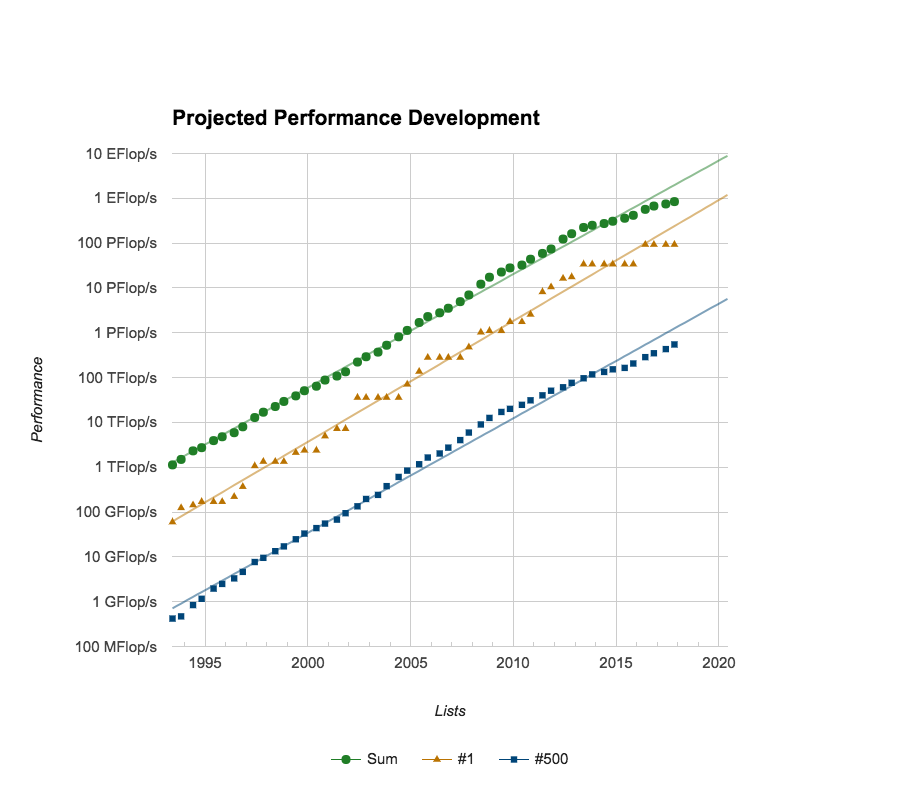
\includegraphics[width=\linewidth]{figures/introduction/top500_list_approximation.png}
\caption{Computational power evolution in the TOP500 list}
\label{fig:intro_top500}
\end{figure}

This linear evolution is not only driven by the shrink in the semiconductor with smaller transistors.
In fact the first one-core Central Processing Units (CPUs) were made using more transistors but also faster frequency.
They later faced limitations to reach high frequencies, because of the power consumption and the inherent cooling of the heat generated by the chip.
This is why, at some point in early twentieth century, IBM proposed the first multi-core processor on the same die, the Power4.
The constructors started to create chips with more than one core to increase the computational power in conjunction with the shrink of semiconductors, answering the constant demand of more powerful devices and allowing the Moore's law to thrive. 
This increase of the overall power of the chip comes with some downside costs in synchronizations steps between the cores for memory access, work sharing and complexity.
The general purpose CPU nowadays features from 2 to less than a hundred of cores on a single chip.\\

In order to reach even more computational power some researchers started to use many-core approaches. 
Using hundreds of cores these devices are using very "simple" computing units, with slow frequency and low power consumption but add more complexity and requirement for their efficient programming with even more synchronizations needed between the cores. 
Usually those many-core architectures are used coupled with a CPU that sends the data and drives them.
Some accelerators can be driven and drive regarding their configuration like the Intel Xeon Phi. 
Usually called accelerators, those devices are used in addition to the host processor to provide their efficient computational power in the key part of execution. 
The most famous accelerators are the Xeon Phi, the General Purpose Graphics Processing Unit (GPGPU) initially used in graphics, Field Programmable Gates Array (FPGA) or dedicated Application-Specific Integrated Circuit (ASIC).
The model using a host with additional device(s) appears and we will mention it as "Hybrid Architecture".
In fact a cluster can be composed of CPUs, CPUs with accelerator(s) of the same kind, CPUs with heterogeneous accelerators or even accelerators like Xeon Phi driving different kinds of accelerators.\\

Since 2013-2014 many companies, like the Gordon Moore's company \textit{Intel} itself, stated that that the Moore's law is over. 
This can be seen on figure~\ref{fig:intro_top500}: on the right part of the graph, the evolution is not linear anymore and tends to decrease slowly in time. 
This can be imputed to two main factors: on one hand, we slowly reach the maximal shrink size of the transistors implying hard to handle side effects. 
On the other hand the power wall implied by the power consumption required by so many transistors and frequency speed on the chip.

Even with all these devices, nowadays supercomputers are facing several problems in their conception and utilization. 
The three mains walls bounding the overall computational power of the machines are the power consumption wall, the communication wall and the memory wall.  
Some subproblems like the the interconnect wall, resilience wall or even the complexity wall also arise and make the task even harder.\\

In this context of doubts and questions about the future of HPC, this study propose several points of view. 
We think that the future of HPC is made with those hybrid architectures or acceleration devices adapted to the need, using well suited API, Framework and code.
We consider that the classical benchmarks, like the TOP500, are not enough to target the main walls of those architectures and especially accelerators. 
Domain scientists applications like physics/astrophysics/chemist/biologist require benchmarks based on more irregular cases with heavy computation, communications and memory accesses. 

In this document we propose a metric that extracts the three main issues of HPC and apply them to accelerated architectures to figure out how to take advantage of those architectures and what the limitations are. 
The first step to this metrics is obtained when merging two characteristic problems and then a third one combining all our knowledge.
The first two are targeting computation and communication wall over very irregular cases with high memory accesses, using an academic combinatorial problem and the Graph500 benchmark. 
The last is a computational scientific problem that covers both difficulties of the previous problems and appears to be hard to implement on supercomputers and even more on accelerated ones.\\

This thesis is composed of 3 parts.

The first develop the state of the art in HPC from the main laws to the hardware. 	
We go through the basic laws from Amdahl's to Gustafson's laws and the specification of speedup and efficiency.
Classical CPUs, GPGPUs and other accelerators are described and discussed regarding the state of the art. 
The main methods of ranking and the issues regarding them are presented.\\ 

In the second part we propose our metric based on characteristic problems to target classical and hybrid architectures.
The Langford problem is described as an irregular and computationally heavy problem.
This shows how the accelerators, in this case GPUs, are able to support the memory and computation wall. 
This allowed us to beat a world record with the last instances of this academic problem.
The Graph500 problem is then proposed as an irregular and communications heavy problem. 
We present our implementation, and more over the logic to take advantage of the GPUs computational power for realistic applications. \\

In the third part we consider a problem that is heavy and irregular regarding to computation and communications.
We analyze it and show that it combine all the previous limitations. 
Then we apply our methodology and show how nowadays supercomputers can overcome those issues. 
This computational science problem is based on the Smoothed Particle Hydrodynamics method.
Based on our global work to efficiently parallelize those kind of production application, we intend to provide an efficient tool for physicists and astrophysicists called FleCSPH. 
The former application we started with was developed on top of the FleCSI framework from the Los Alamos National Laboratory it allowed us to exchange directly with the LANL domain scientists on their need.\\

The last part will conclude on this work and results and show some of the main prospects of this study and my future researches. 
% Chapter One
\part{HPC and Exascale}
\chapter*{Introduction}

High Performance Computing, HPC, does not find a strict definition. 
Since computer creation, first dedicated for balistic purposes, domain scientists developped their tool to perform computations. 
Then, in front of the complexity of building such machines, HPC became a dedicated field of research. 

Computer scientists interested in HPC will have to focus on several domains. 
\begin{itemize}
\item The energy consumption, mainly directed by the hardware producers. 
\item The computational power, how to take advantages of the ressources ? 
\item The communication, because such machines are constructed over several machines or nodes. 
\end{itemize}

Domain scientists are also involved directly in HPC with their software and redefining the structure based on their needs and usages. 

%%%%%%%%%%%%%%%%%%%%%%%%%%%%%%%%%%%%%%%%%%%%%%%%%%%%%%%%%%%%%%%%%%%%%
%																	%
%	CHAPTER ONE, THEORY of HPC										%
%																	%
%%%%%%%%%%%%%%%%%%%%%%%%%%%%%%%%%%%%%%%%%%%%%%%%%%%%%%%%%%%%%%%%%%%%%

%%%%%%%%%%%%%%%%%%%%%%%%%%%%%%%%%%%%%%%%%%%%%%%%%%%%%%%%%%%%%%%%%%%%%
%                                                                   %
%	CHAPTER ONE, MODELS of HPC                                       %
%                                                                   %
%%%%%%%%%%%%%%%%%%%%%%%%%%%%%%%%%%%%%%%%%%%%%%%%%%%%%%%%%%%%%%%%%%%%%

\chapter{Models of HPC}

\section{Introduction}

High Performance Computing (HPC) takes his roots from the beginning of computer odyssey in the middle of 20th century.
A lot of rules, observations, theories emerged from it and most of the Computer Science fields. 
In order to understand and characterize HPC and supercomputers, some knowledge on theory is required. 
This part describes the Von Neumann model, the generic model of sequential computer on which every nowadays machine is built.
It is presented along with the Flynn taxonomy that is a classification of the different execution models. 
We also present the different memory models based on those elements. 

Then we give more details on what is parallelism and how to reach performances though it. 
And thus we define what performance implies in HPC. 
The Amdahl's and Gustafson's laws are presented and detailed along with the strong and weak scaling used in our study. 

\section{Von Neumann Model}
\index{Von Neumann Model}
First computers, in early 20th, were built using vacuum tubes making them high power consuming, hard to maintain and expansive to build.
The most famous of first vacuum tubes supercomputers, the ENIAC, was based on a decimal system.
It might be the most known of first supercomputers but the real revolution came from its successor.
In 1944 the first binary system based computer, called the Electric Discrete Variable Automatic Computer (EDVAC), was created. 
In the EDVAC team, a physicists described the logical model of this computer and provides a model on which every nowadays computing device is based. 

\begin{figure}
\centering 
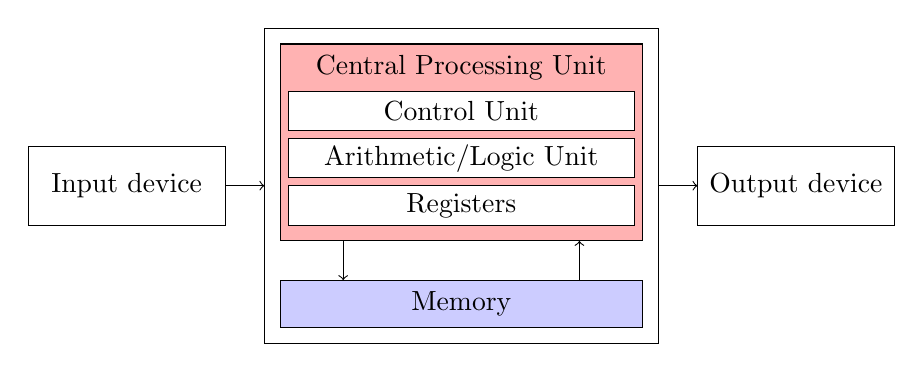
\begin{tikzpicture}
\draw (3,0) rectangle (8,4);
\draw (3.2,1.3) [fill=red!30] rectangle (7.8,3.8);
\node at (5.5,3.5) {Central Processing Unit};

\draw (3.3,1.5) [fill=white] rectangle (7.7,2.) node[pos=.5] {Registers};
\draw (3.3,2.1) [fill=white] rectangle (7.7,2.6) node[pos=.5] {Arithmetic/Logic Unit};
\draw (3.3,2.7) [fill=white] rectangle (7.7,3.2) node[pos=.5] {Control Unit};

\draw (0,1.5) rectangle (2.5,2.5) node[pos=.5] {Input device};
\draw (8.5,1.5) rectangle (11,2.5) node[pos=.5] {Output device};
\draw [->] (2.5,2) -- (3,2);
\draw [->] (8,2) -- (8.5,2);

\draw (3.2,.2) [fill=blue!20] rectangle (7.8,.8) node[pos=.5] {Memory};
\draw [->] (4,1.3) -- (4,.8);
\draw [->] (7,.8) -- (7,1.3);
\end{tikzpicture}
\caption{Von Neumann model}
\label{fig:1_HPC:von_neumann_model}
\end{figure}

John Von Neumann published its \textit{First Draft of a Report on the EDVAC}~\cite{von1993first} in 1945. 
Extracted from this work, the model known as the Von Neumann model or more generally Von Neumann Machine appears. 
The model is presented on figure~\ref{fig:1_HPC:von_neumann_model}.

On that figure we identify three parts, the input and output devices and, in the middle, the computational device itself. 
\paragraph{Input/Output devices}
The input and output devices are used to store in a read/write way data. 
They can be represented as hard drives, solid state drives, monitors, printers or even mouse and keyboard.
The input and output devices can also be the same, reading and writing in the same area.\\

Inside the computational device we find the memory, for the most common nowadays architectures it can be considered as a Random Access Memory (RAM). 
Several kind of memory exists and will be discussed later. 

\paragraph{Central Processing Unit}
\index{Central Processing Unit}
The Central Processing Unit, CPU, is composed of several elements in this model. 
On one hand, the \textit{Arithmetic and Logic Unit}, ALU, which takes as input one or two values, the data, and apply an operation on them. 
They can be either logics with operations such as AND, OR, XOR, etc. or arithmetics with operations such as ADD, MUL, SUB, etc. 
Those operations can be way more complex on modern CPUs. 
On the other hand, we find the \textit{Control Unit}, CU, which controls the data carriage to the ALU from the memory and the operation to be perform on data.
It is also the part that takes care of the Program Counter (PC): the address of the next instruction in the program. 
We can also identify the \textit{Registers} section which represents data location used for both ALU and CU to store temporary results, the current instruction address, etc. 
Some representations may vary, the \textit{Registers} can be represented directly inside the ALU or the CU. 
\paragraph{Buses}
The links between those elements are called Buses and can be separated in data buses, control buses and addresses buses.
They will have a huge importance for the first machine optimization, growing the size of the buses from 2, 8, 16, 32, 64 and even more for vector machine with 128 and 256 bits.\\

The usual processing flow on such an architecture can be summarized as a loop: 
\begin{itemize}[noitemsep,nolistsep]
\item[-] Fetch instruction at current PC from memory;
\item[-] Decode instruction using the Instruction Set Architecture (ISA). Known ISA are Reduce Instruction Set Computer architecture (RISC) and Complex Instruction Set Computer architecture (CISC);
\item[-] Evaluate operand(s) address(es);
\item[-] Fetch operand(s) from memory;
\item[-] Execute operation(s). With some instructions sets and new architectures several similar operations can be processed in the same clock time;
\item[-] Store results, increase PC.\\
\end{itemize}

Every devices or machines we describe in the next chapter have this architecture as a basis. 
One will consider execution models and architecture models to characterize HPC architectures.

\section{Flynn taxonomy and execution models}
\index{Flynn taxonomy}
The Von Neumann model gives us a generic idea of how a computational unit is fashioned. 
The constant demand in more powerful computers required the scientists to find more way to provide this computational power.
In 2001, IBM proposed the first multi-core processor on the same die, the Power4 with its 2 cores.
This evolution required new paradigms.
A right characterization is then essential to be able to target the right architecture for the right purpose. 
The Flynn taxonomy presents a hierarchical organization of computation machines and executions models.

\begin{table}
\centering
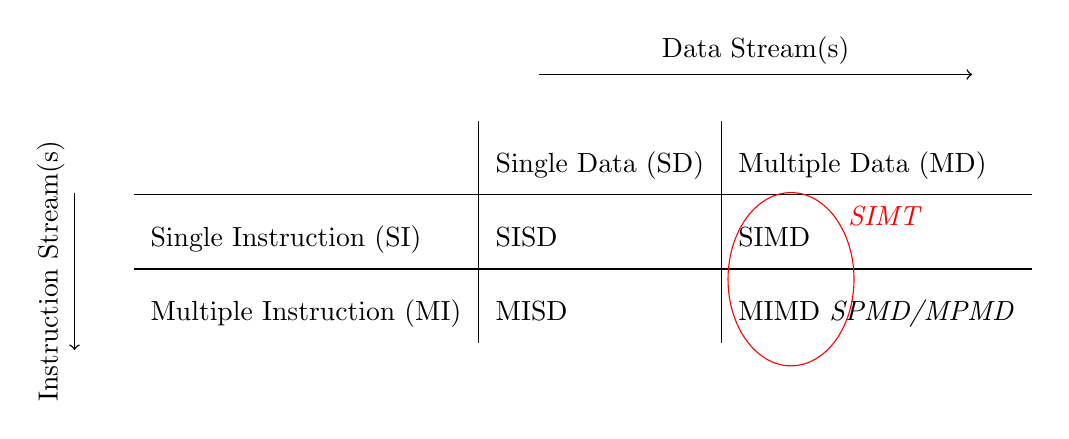
\begin{tikzpicture}
\node (table) {\arraycolsep=1.4pt\def\arraystretch{2.2}
\begin{tabular}{l | l | l}
 & Single Data (SD) & Multiple Data (MD) \\
 \hline 
Single Instruction (SI) & SISD & SIMD \\
\hline 
Multiple Instruction (MI) & MISD & MIMD \textit{SPMD/MPMD} \\
\end{tabular}
};
\draw [->,line width=.5pt] (-0.5,2) -- (5,2) node[midway, above] {Data Stream(s)};
\draw [->,line width=.5pt] (-6.4,0.5) -- (-6.4,-1.5) node[rotate=180,sloped, midway, above] {Instruction Stream(s)};
\draw [red] (2.7,-.6) ellipse (.8cm and 1.1cm) node[xshift=1.2cm,yshift=.8cm] {\textit{SIMT}};
%\draw[decoration={brace,raise=5pt},line width=1pt,decorate]
%  (5,0.4) -- node[right=6pt,yshift=5pt] {\textit{SIMT}} (5,-1.5);
\end{tikzpicture}
\caption{Flynn taxonomy for execution models completed with SPMD and SIMT models}
\label{tab:1_HPC:taxonomy_flynn}
\end{table}

\begin{figure}
\resizebox {.24\columnwidth} {!} {
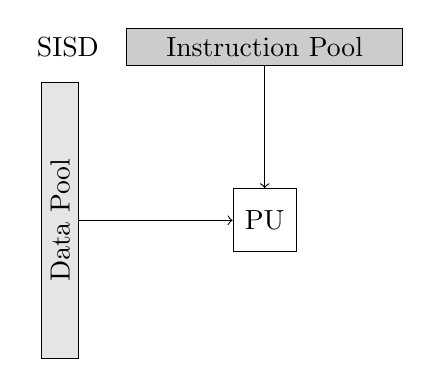
\begin{tikzpicture}
\draw (0.1,5.2) node {SISD}; 
\node (rect) at (2.6,5.2) [draw,minimum width=3.5cm,fill=black!20] (ip) {Instruction Pool};
\node (rect) at (0,3) [rotate=90,draw,minimum width=3.5cm,fill=black!10] (dp) {Data Pool};
\node (rect) at (2.6,3) [draw,minimum width=.8cm,minimum height=.8cm] (pu1) {PU};
\draw [->] (ip) -- (pu1);
\draw [->] (dp) -- (pu1);
\end{tikzpicture}
}
\resizebox {.24\columnwidth} {!} {
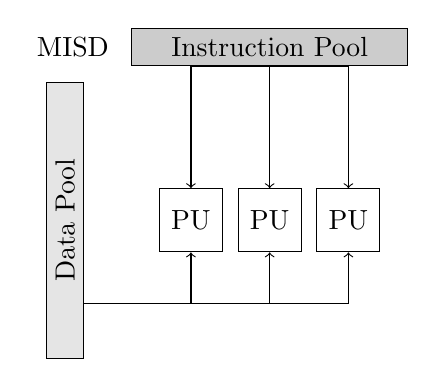
\begin{tikzpicture}
\draw (0.1,5.2) node {MISD}; 
\node (rect) at (2.6,5.2) [draw,minimum width=3.5cm,fill=black!20] (ip) {Instruction Pool};
\node (rect) at (0,3) [rotate=90,draw,minimum width=3.5cm,fill=black!10] (dp) {Data Pool};
\node (rect) at (1.6,3) [draw,minimum width=.8cm,minimum height=.8cm] (pu1) {PU};
\node (rect) at (3.6,3) [draw,minimum width=.8cm,minimum height=.8cm] (pu2) {PU};
\node (rect) at (2.6,3) [draw,minimum width=.8cm,minimum height=.8cm] (pu3) {PU};

\draw[<-] (pu1.north) |-  (ip.south); 
\draw[<-] (pu2.north) |-  (ip.south);
\draw[<-] (pu3.north) |-  (ip.south);

\draw[<-]  (pu1.south) |- ([yshift=-30pt]dp.south);
\draw[<-]  (pu2.south) |- ([yshift=-30pt]dp.south);
\draw[<-]  (pu3.south) |- ([yshift=-30pt]dp.south);

\end{tikzpicture}
}
\resizebox {.24\columnwidth} {!} {
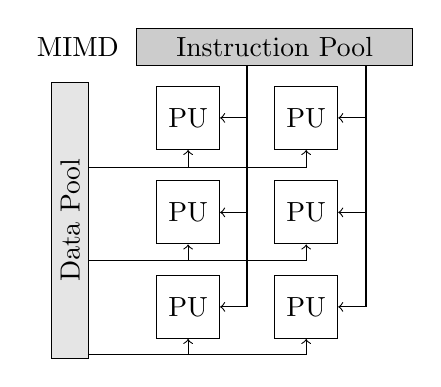
\begin{tikzpicture}
\draw (0.1,5.2) node {MIMD}; 
\node (rect) at (2.6,5.2) [draw,minimum width=3.5cm,fill=black!20] (ip) {Instruction Pool};
\node (rect) at (0,3) [rotate=90,draw,minimum width=3.5cm,fill=black!10] (dp) {Data Pool};
\node (rect) at (1.5,4.3) [draw,minimum width=.8cm,minimum height=.8cm] (pu1) {PU};
\node (rect) at (1.5,3.1) [draw,minimum width=.8cm,minimum height=.8cm] (pu2) {PU};
\node (rect) at (1.5,1.9) [draw,minimum width=.8cm,minimum height=.8cm] (pu3) {PU};
\node (rect) at (3,4.3) [draw,minimum width=.8cm,minimum height=.8cm] (pu4) {PU};
\node (rect) at (3,3.1) [draw,minimum width=.8cm,minimum height=.8cm] (pu5) {PU};
\node (rect) at (3,1.9) [draw,minimum width=.8cm,minimum height=.8cm] (pu6) {PU};

\draw[<-]  (pu1.south) |- ([yshift=19pt]dp.south);
\draw[<-]  (pu4.south) |- ([yshift=19pt]dp.south);

\draw[<-]  (pu2.south) |- ([yshift=-14.5pt]dp.south);
\draw[<-]  (pu5.south) |- ([yshift=-14.5pt]dp.south);

\draw[<-]  (pu3.south) |- ([yshift=-48.5pt]dp.south);
\draw[<-]  (pu6.south) |- ([yshift=-48.5pt]dp.south);

\draw[->] ([xshift=-10pt]ip.south) |- (pu1.east);
\draw[->] ([xshift=-10pt]ip.south) |- (pu2.east);
\draw[->] ([xshift=-10pt]ip.south) |- (pu3.east);

\draw[->] ([xshift=33pt]ip.south) |- (pu4.east);
\draw[->] ([xshift=33pt]ip.south) |- (pu5.east);
\draw[->] ([xshift=33pt]ip.south) |- (pu6.east);

%\draw[<-]  (pu2.south) |- ([yshift=-30pt]dp.south);
%\draw[<-]  (pu3.south) |- ([yshift=-30pt]dp.south);

%\draw [->] (ip) -- (pu1);
%\draw [->] (dp) -- (pu1);
\end{tikzpicture}
}
\resizebox {.24\columnwidth} {!} {
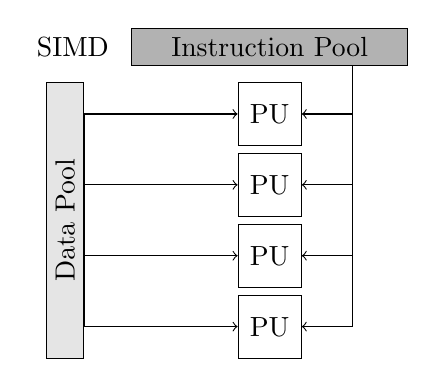
\begin{tikzpicture}
\draw (0.1,5.2) node {SIMD}; 
\node (rect) at (2.6,5.2) [draw,minimum width=3.5cm,fill=black!30] (ip) {Instruction Pool};
\node (rect) at (0,3) [rotate=90,draw,minimum width=3.5cm,fill=black!10] (dp) {Data Pool};
\node (rect) at (2.6,4.35) [draw,minimum width=.8cm,minimum height=.8cm] (pu1) {PU};
\node (rect) at (2.6,3.45) [draw,minimum width=.8cm,minimum height=.8cm] (pu2) {PU};
\node (rect) at (2.6,2.55) [draw,minimum width=.8cm,minimum height=.8cm] (pu3) {PU};
\node (rect) at (2.6,1.65) [draw,minimum width=.8cm,minimum height=.8cm] (pu4) {PU};
%\draw [->] ([yshift=2.35cm]dp) -- (pu1);
\draw[->] (dp.south) |- (pu1.west);
\draw[->] (dp.south) |- (pu2.west);
\draw[->] (dp.south) |- (pu3.west);
\draw[->] (dp.south) |- (pu4.west);

\draw[->] ([xshift=30pt]ip.south) |- (pu4.east);
\draw[->] ([xshift=30pt]ip.south) |- (pu3.east);
\draw[->] ([xshift=30pt]ip.south) |- (pu2.east);
\draw[->] ([xshift=30pt]ip.south) |- (pu1.east);
%\draw[arrow] (Small2B.north)--(Small2B|-Big2.south);s
%\draw [->] (dp) -- (pu1);
\end{tikzpicture}
}
\caption{Flynn taxonomy schematic representation of execution models}
\label{fig:1_HPC:flynn_taxonomy}
\end{figure}

In this classification~\cite{flynn1972some} from 1972, Michael J. Flynn presents the SISD, MISD, MIMD, and SIMD models represented on in table~\ref{tab:1_HPC:taxonomy_flynn} and figure~\ref{fig:1_HPC:flynn_taxonomy}.
Every of those execution model corresponds to a specific machine and function.

\subsection{Single Instruction, Single Data: SISD}
This is the model corresponding to a single core CPU like in the Von Neumann model. 
This sequential model takes one instruction, operates on one data and the result is then stored and the process continues over. 
SISD is important to consider for a reference computational time and will be taken in account in the next part for Amdahl's and Gustafson's laws.

\subsection{Multiple Instructions, Single Data: MISD}
This model can correspond to a pipelined computer.
Different operations are applied to the datum, which is transfered to the next computational unit and so on. 
This is the least common execution model.


\subsection{Multiple Instructions, Multiple Data: MIMD}
In MIMD every element executes its own instructions on its own data set. 
This can represent the behavior of a processor using several cores, threads or even the different nodes of a supercomputer cluster. 
Two subcategories are identified in this model: SPMD and MPMD.

\subsubsection{SPMD}
The Single Program Multiple Data model, SPMD, is the most famous parallelism way for HPC purpose: each process executes the same program. 
At opposite to SIMD the programs are the same but does not share the same instruction counter. 
This model was proposed for the first time in \cite{darema1988single} in 1988 using Fortran.
This is the common approach working with runtime like MPI. 
The programs are the same and the execution similar but based on their ID the processes will target different data. 

\subsubsection{MPMD}
The Multiple Program Multiple Data model is also know for HPC. 
Generally with a separation between a main program generating data for sub-programs. 
This is the model on which we work in part II regarding the Langford problem resolution using a master program generating tasks for the slaves CPUs/GPGPUs programs.

\subsection{Single Instruction, Multiple Data: SIMD}
This execution model corresponds to a many-core architecture like a GPU. 
SIMD can be extended from 2 to 16 elements for classical CPUs to hundreds and even thousands of core for GPGPUs. 
In the same clock cycle, the same operation is executed on every process on different data. 
A good example is the work on matrices with stencils: same instruction executed on every element of the matrix. 

\subsection{SIMT}
\index{Single Instruction Multiple Threads}
We find another characterization to describe the new GPUs architecture: Single Instruction, Multiple Threads. 
This appears in one of NVIDIA's company paper~\cite{lindholm2008nvidia}. 
This model describes a combination of MIMD and SIMD architectures, every block of threads is working with the same control processor on different data and every block has its own instruction counter.  
This is the model we describe in part \ref{sec:CUDA} used for the \textit{warps} model in NVIDIA CUDA.

\section{Memory}
\label{sec:NORMA}
In addition of the execution model and parallelism the memory access patterns have a main role on performances especially in SIMD and MIMD. 
In this classification we identify three categories: UMA, NUMA and NoRMA for shared and distributed cases. 
This model have been pointed out in the Johnson's taxonomy\cite{johnson1988completing}.

%We can also find Error-Correcting Code, ECC, memory which implements a bunch of data correction algorithm to guaranty the validity of them when error is not allowed. 

%\todo{MCDRAM}
%\todo{3D memory}

\begin{figure}
\centering 
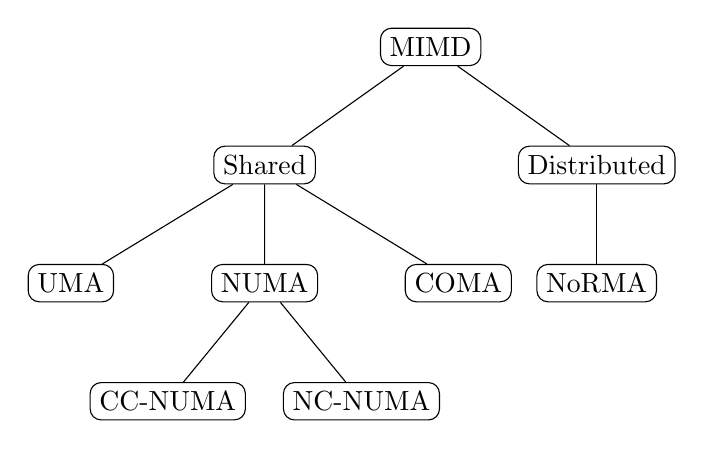
\begin{tikzpicture}[
   every node/.style = {
   level distance=1em,
   shape=rectangle, 
   rounded corners,
   draw, 
   align=center,
    top color=white%, 
   % bottom color=blue!20
   }]]
   \node {MIMD} [sibling distance=12em]
   child { node {Shared} [sibling distance=7em]
   child{node {UMA}} 
   child{node {NUMA}
   child{node {CC-NUMA}}
   child{node {NC-NUMA}}
   }
   child{node {COMA}}
   }
   child { node {Distributed}
   child { node {NoRMA}}
   };
\end{tikzpicture}
\caption{MIMD memory models}
\label{fig:1_HPC:mimd_memory_model}
\end{figure}

Those different types of memory for SIMD/MIMD model are summed up in figure~\ref{fig:1_HPC:mimd_memory_model}.

\subsection{Shared memory}
%In case of the SISD the memory access is just serial and no really rules needs to be set for its usage. 
Several kind of memory models are possible when it comes to multi-threaded and multi-cores execution models like MIMD or SIMD.
We give a description of the most common shared memories architectures. 

\hspace*{-2cm}
\begin{figure}
\centering 
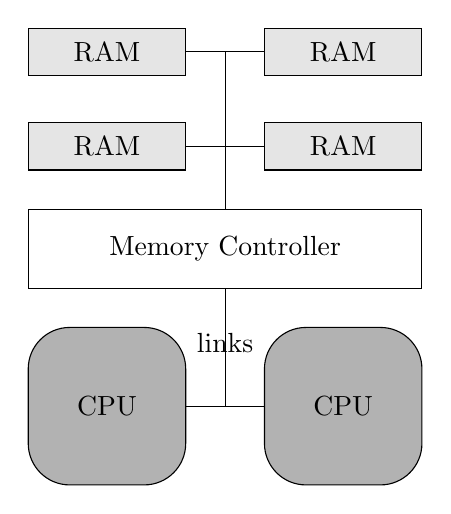
\begin{tikzpicture}
   \draw [rounded corners=15pt,fill=black!30] (0,0) rectangle (2,2) node[pos=.5] {CPU};
   \draw [rounded corners=15pt,fill=black!30] (3,0) rectangle (5,2) node[pos=.5] {CPU};

   \draw (0,2.5) rectangle (5,3.5) node[pos=.5] {Memory Controller};

   \draw (0,4) [fill=black!10] rectangle (2,4.6) node[pos=.5] {RAM};
   \draw (0,5.2) [fill=black!10] rectangle (2,5.8) node[pos=.5] {RAM};

   \draw (3,4) [fill=black!10] rectangle (5,4.6) node[pos=.5] {RAM};
   \draw (3,5.2) [fill=black!10] rectangle (5,5.8) node[pos=.5] {RAM};

   \draw [-] (2,1) -- (3,1);
   \draw [-] (2.5,1) -- (2.5,2.5);
	%\node at (2.5,2.2) {SDR, DDR, QDR};
	\node at (2.5,1.8) {links};

	\draw [-] (2.5,3.5) -- (2.5,5.5);
	\draw [-] (2,4.3) -- (3,4.3);
	\draw [-] (2,5.5) -- (3,5.5);
\end{tikzpicture}
\hspace{2cm}
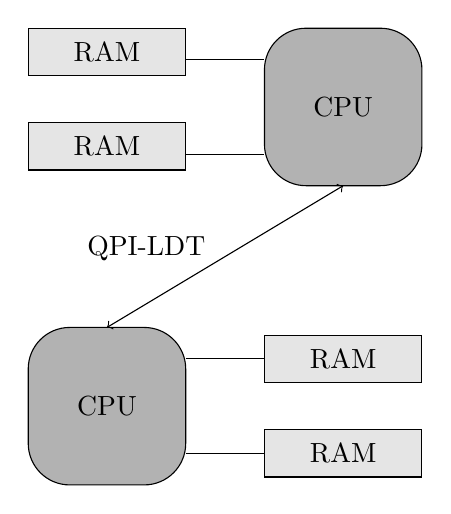
\begin{tikzpicture}
	\draw [rounded corners=15pt,fill=black!30] (0,0) rectangle (2,2) node[pos=.5] {CPU};
	\draw (3,0.1) [fill=black!10] rectangle (5,0.7) node[pos=.5] {RAM};
	\draw (3,1.3) [fill=black!10] rectangle (5,1.9) node[pos=.5] {RAM};
	\draw [-] (2,0.4) -- (3,0.4);
	\draw [-] (2,1.6) -- (3,1.6);

	\draw [rounded corners=15pt,fill=black!30] (3,3.8) rectangle (5,5.8) node[pos=.5] {CPU};
	\draw (0,4) [fill=black!10] rectangle (2,4.6) node[pos=.5] {RAM};
	\draw (0,5.2) [fill=black!10] rectangle (2,5.8) node[pos=.5] {RAM};
	\draw [-] (2,4.2) -- (3,4.2);
	\draw [-] (2,5.4) -- (3,5.4);

	\draw [<->] (1,2) -- (4,3.8);
	\node at (1.5,3) {QPI-LDT};
\end{tikzpicture}
%\hspace{1cm}
%\begin{tikzpicture}
%	\draw [rounded corners=15pt] (1,0) rectangle (3,2) node[pos=.5] {CPU};
%	\draw [rounded corners=15pt] (1,3.8) rectangle (3,5.8) node[pos=.5] {CPU};
%
%	\draw (0,2.1) rectangle (2,2.8) node[pos=.5] {RAM};
%	\draw (0,3.2) rectangle (2,3.8) node[pos=.5] {RAM};
%	
%	\draw (3,2.2) rectangle (5,2.8) node[pos=.5] {RAM};
%	\draw (3,2.2) rectangle (5,3.8) node[pos=.5] {RAM};
%
%\end{tikzpicture}
\caption{UMA vs NUMA memory models}
\label{fig:1_HPC:UMA_NUMA}
\end{figure}

\subsubsection{UMA}
\index{Unified Memory Access}
The Uniform Memory Access is a global memory shared by every threads or cores. 
In UMA every processor uses its own cache as local private memory. 
The addresses can be accessed directly by each processor which makes the access time ideal. 
The downside is that more processors require more buses and thus UMA is hardly scalable. 
The cache consistency problem also appears in this context and will be discussed in next part. 
Indeed, if a data is loaded in one processor cache and modified, this information need to be spread to the memory and maybe other processes cache. 

With the arising of accelerators like GPUs and their own memory, some constructors found ways to create UMA with heterogeneous memory. 
AMD creates the heterogeneous UMA, hUMA~\cite{rogers2013amd} in 2013, allowing CPU and GPU to target the same memory area.

\subsubsection{NUMA}
\index{Non Unified Memory Access}
In Non Unified Memory Access every processor have access to its own private memory but allows other processors to access it though Lightning Data Transport, LDT or Quick Path Interconnect, QPI, for Intel architectures. 

As we mentioned for the UMA memory, even if the processors does not directly access to the memory cache coherency is important. 
Two methods are possible: on one hand, the most used is Cache-Coherent NUMA (CC-NUMA) were protocols are used to keep data coherency through the memory. On the other hand No Cache NUMA (NC-NUMA) forces the processes to avoid cache utilization and write results in main memory losing all the benefits of caching data. 

\subsubsection{COMA}
\index{Cache-Only Memory Access}
In Cache-Only Memory Accesses, the whole memory is see as a cache from every processes.
An \textit{Attraction memory} pattern is used to \textit{attract} the data near the process that will use those data. 
This model is less commonly use and lead to, in best cases, same results as NUMA.

\subsection{Distributed memory}
\index{No Remote Memory Access}
The previous models are based on shared memory, in the case where the processes can access memory of their neighbors processes. 
In some cases, like supercomputers, it would be too heavy for processors to handle the requests of all the others through the network. 
Each process or node will then possess its own local memory, that can be share with local processes. 
Then, in order to access to other nodes memory, communications through the network have to be done and copied in local memory. 
This distributed memory is called No Remote Memory Access (NoRMA).

\section{Performances characterization in HPC}
In the previous parts we described the different executions models, characterizations and memory models for HPC. 
Based on those tools we need to be able to emphasis the performances of a computer and a cluster. 

The performance can be of several kind. 
It can first be define by the speed of the processor itself with the frequency defined in GHz. 
This information is not perfect because the ALU is not busy all the time due to memory accesses, communications or side effects. 
It can be used to estimate the highest computational power of a machine. 
We define the notion of \textit{cycle} to be the number that determine the speed of a processor. 
This is the amount of time between two pulses of the oscillator at the best frequency. 
Higher cycles per seconds is better. 

\subsection{FLOPS}

\index{Floating-point Operations Per Second}
The Floating point Operations Per Second considers the number of floating-point operation that the system will executes in a second. 
They are a unit of performance for computers. 
Higher FLOPS is better. 
This is also the scale used to consider supercomputers computational power. 
For a cluster we can compute the theoretical FLOPS (peak) based on the processor frequency in GHz with:
\begin{equation}
FLOPS_{cluster} = \#nodes \times \frac{\#sockets}{\#node} \times \frac{\#cores}{\#socket} \times \frac{\#GHz}{\#core} \times \frac{FLOPS}{cycle}
\end{equation}
With $\#nodes$ the number of computational node of the system, $\frac{\#sockets}{\#node}$ the number of sockets (=processors) per node, $\frac{\#cores}{\#socket}$ the number of cores in the processor, $\frac{\#GHz}{\#core}$ the frequency of each core and finally $\frac{\#FLOP}{\#cycle}$ the number of floating-point operations per cycles for this architecture. 


On figure~\ref{tab:1_HPC:flops_year}, the scale of FLOPS and the year of the first world machine is presented.
The next milestone, the exascale, is expected to be reach near 2020.  

\begin{table}
\[\arraycolsep=1.4pt\def\arraystretch{2.2}
\begin{tabular}{| l | l | l || l | l | l |}
\hline
	%\rowstyle{\bfseries}
	\textbf{Name} & \textbf{FLOPS} & \textbf{Year} & \textbf{Name} & \textbf{FLOPS} & \textbf{Year} \\
	\hline
	\hline
	kiloFLOPS & $10^{3}$ & & petaFLOPS  & $10^{15}$ & 2005 \\ 
	\hline
	megaFLOPS & $10^{6}$ & & exaFLOPS   & $10^{18}$ & 2020 ? \\
	\hline
	gigaFLOPS & $10^{9}$ & $\approx$ 1980  & zettaFLOPS & $10^{21}$ & \\
	\hline
	teraFLOPS & $10^{12}$ & 1996 & yottaFLOPS & $10^{24}$ & \\
	\hline
	\end{tabular}
	\]
	\caption{Floating-point Operation per Second and years of reach in HPC.}
	\label{tab:1_HPC:flops_year}
\end{table}

FLOPS is the main way to represent a computer's performance but other ways exists like Instructions Per Seconds (IPS), Instructions per Cycle (IPC) or Operations Per Second (OPS).
Some benchmarks also provide their own metrics. 

\subsection{Power consumption}
Another way to consider machine performance is to estimate the number of operations regarding the power consumption. 
It considers all the previous metrics like FLOPS, IPS, IPC or OPS. 
Benchmarks like the Green500 consider the FLOPS delivered over the watts consumed. 
For nowadays architectures the many-cores architectures like GPUs seems to deliver the best FLOPS per watt ratio.

\subsection{Scalability}
The scalability express the way a program react to parallelism. 
When an algorithm is implemented on a serial machine and is ideal to solve a problem, one may consider to use it on more than one core, socket, node or even cluster. 
Indeed, one may expect less computation time, bigger problem or a combination of both while using more resources. 
This is completely dependent of the algorithm's parallelization and is expressed through scalability. 
A scalable program will scale on as many processors as provided, whereas a poorly scalable one will give same of even worst results as the serial code.  
Scalability can be approach using speedup and efficiency.

\subsection{Speedup and efficiency}
The latency is the time required to complete a task in a program.
\index{Latency} 
Lower latency is better. 

The speedup compares the latency of both sequential and parallel algorithm. 
In order to get relevant results, one may consider the best serial program against the best parallel implementation.

Considering $n$, the number of processes, and $n=1$ the sequential case.
$T_n$ is the execution time working on $n$ processes and $T_1$ working on one process: the sequential execution time. 
The speedup can be defined using the latency by the formula: 
\index{Speedup}
\begin{equation}
\text{speedup} = S_n =  \frac{T_1}{T_n}
\end{equation}

\begin{figure}
\centering 
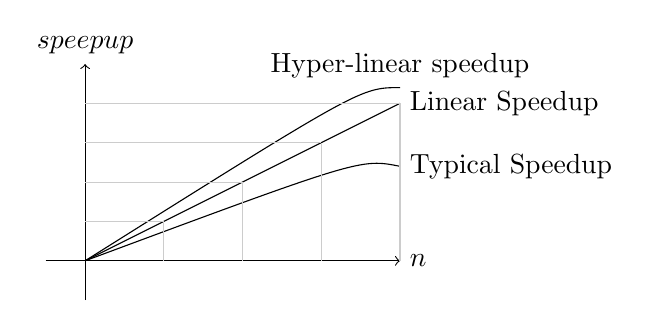
\begin{tikzpicture}
	\draw[->] (-.5,0) -- (4,0) node[right] {$n$};
	\draw[->] (0,-.5) -- (0,2.5) node[above] {$speepup$};
	\draw (0,0) -- (4,2) node[right] {\text{Linear Speedup}};
	\draw (0,0) .. controls (3.5,1.3) .. (4.,1.2) node[right] {\text{Typical Speedup}} ;
	\draw (0,0) .. controls (3.5,2.2) .. (4.,2.2) node[above] {\text{Hyper-linear speedup}} ;
   \draw[black!20] (1,0) -- (1,.5);
   \draw[black!20] (2,0) -- (2,1);
   \draw[black!20] (3,0) -- (3,1.5);
   \draw[black!20] (4,0) -- (4,2);
   \draw[black!20] (0,.5) -- (1,.5);
   \draw[black!20] (0,1) -- (2,1);
   \draw[black!20] (0,1.5) -- (3,1.5);
   \draw[black!20] (0,2) -- (4,2);
\end{tikzpicture}
\caption{Observed speedup: linear, typical and hyper-linear speedups}
\label{fig:1_HPC:speedup_obs}
\end{figure}

As shown on figure \ref{fig:1_HPC:speedup_obs} several kind of speedup can be observed. 
\paragraph{Linear, reference speedup: }
The linear speedup usually represents the target for every program in HPC. 
Indeed, having the speedup growing linearly as the number of processors grows is the ideal case. 
Codes fall typical into two cases, typical and hyper-linear speedup. 
\paragraph{Typical speedup: }
This represents the most common observed speedup. 
As the number of processors grows, the program faces several of the HPC walls like communications wall or memory wall. 
The increasing number of computational power is reduced to the sequential part or lose time in communications/exchanges. 
\paragraph{Hyper-linear speedup: }
In some cases we observe an hyper-linear speedup, meaning that the results in parallel are even better than the ideal case. 
This can occur if the program fits exactly in memory for less data on each processor or even fit perfectly for the cache utilization. 
The parallel algorithm can also be way more efficient than the sequential one.\\

In addition to speedup, the efficiency is defined by the speedup divided by the number of workers: 
\index{Efficiency}
\begin{equation}
\text{efficiency} = E_n = \frac{S_n}{n} = \frac{T_1}{nT_n}
\end{equation}
The efficiency, usually expressed in percent, represents the evolution of the code stability to growing number of processors. 
As the number of processes grows, a scalable application will keep an efficiency near 100\%.

\subsection{Amdahl's and Gustafson's law}
The Amdahl's and Gustafson's laws are ways to evaluate the maximal possible speedup for an application taking in account different characteristics. 

\subsubsection{Amdahl's law}
\index{Amdahl's law}
The Amdahl's law\cite{amdahl1967validity} is used to find the theoretical speedup in latency of a program.
We can separate a program into two parts, the one that can be execute in parallel and the one that is sequential. 
The law states that even if we reduce the parallel part using an infinity of processes the sequential part will reach 100\% of the total computation time. 

Extracted from the Amdahl paper the law can be written as: 

\begin{equation}
S_n = \frac{1}{Seq + \frac{Par}{n}}
\end{equation}

Where $Seq + Par = 1$ and $Seq$ and $Par$ respectively the sequential and parallel ratio of a program.
Here if we use up to $n=\inf$ processes, $S_n \leq \frac{1}{Seq}$ the sequential part of the code become the most time consuming. 

And the efficiency become:
\begin{equation}
E_n = \frac{1}{n\times Seq + Par}
\end{equation}

\begin{figure}
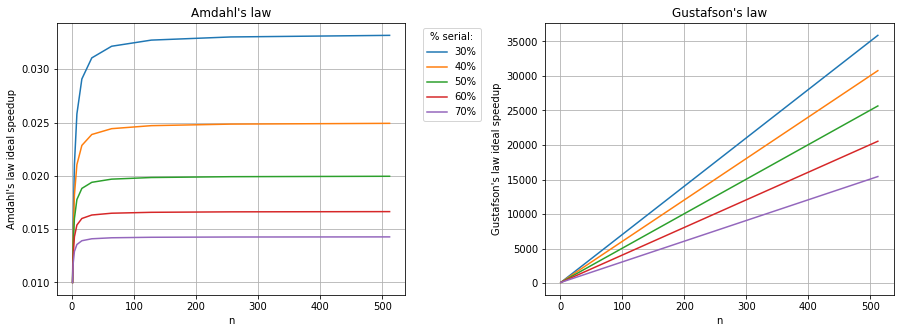
\includegraphics[width=\textwidth]{\locpath/figures/chap1/speedup_laws.png}
\caption{Theoretical speedup for Amdahl's (left) and Gustafson's (right) law}
\label{fig:1_HPC:speedup_laws}
\end{figure}

A representation of Amdahl's speedup is presented on Fig.~\ref{fig:1_HPC:speedup_laws} with varying percentage of serial part. 
The parallel part is like $Par = (100-Ser)\%$.

\subsubsection{Gustafson's law}
\index{Gustafson's law}
The Amdahl's law is focused on time with problem of the same size. 
John L. Gustafson's idea is that using more computational units, the problem size can grow accordingly. 
He considered a constant computation time with evolving problem, growing the size accordingly to the number of processes. 
Indeed the parallel part grows as the problem size do, reducing the percentage of the serial part for the overall resolution.

The speedup can now be estimated by:
\begin{equation}
S_n = Seq + Par \times n
\end{equation}

And the efficiency: 
\begin{equation}
E_n = \frac{Seq}{n} + Par
\end{equation}


Both Amdahl's and Gustafson's law are applicable and they represent two solution to check the speedup of our applications. 
\textbf{The strong scaling}\index{Strong scaling}, looking at how the computation time vary evolving only the number of processes, not the problem size. 
\textbf{The weak scaling}\index{Weak scaling}, at opposite to strong scaling we look how the computation time evolute varying the problem size keeping the same amount of work per processes. 

\section{Conclusions}

In this chapter we presented the different basic tools to be able to understand HPC: the Von Neumann model that is implemented in every nowadays architecture; the Flynn taxonomy that is in constant evolution with new paradigms like recent SIMT from NVIDIA. 
We also presented the memory types that will be use at different layers in our clusters, from node memory, CPU-GPGPU shared memory space to global fast shared memory. 
We finished by presenting the most important laws with Amdahl's and Gustafson's laws.
We introduced the concept of strong and weak scaling that will lead our tests through all the examples in Part II and Part III.

Those models have now to be confronted to the reality with hardware implementation and market reality, the vendors. 
The next part introduces chronologically hardware and their optimization and always keeps a link with the models presented in this part. 
As there is always a gap between models and implementation we will have to find way to rank and characterize those architecture. 
This will be discuss in the last chapter. 



%%%%%%%%%%%%%%%%%%%%%%%%%%%%%%%%%%%%%%%%%%%%%%%%%%%%%%%%%%%%%%%%%%%%%
%																	%
%	CHAPTER TWO, HARDWARE IN HPV									%
%																	%
%%%%%%%%%%%%%%%%%%%%%%%%%%%%%%%%%%%%%%%%%%%%%%%%%%%%%%%%%%%%%%%%%%%%%

%%%%%%%%%%%%%%%%%%%%%%%%%%%%%%%%%%%%%%%%%%%%%%%%%%%%%%%%%%%%%%%%%%%%%
%                                                                   %
%	CHAPTER TWO, HARDWARE IN HPC                                    %
%                                                                   %
%%%%%%%%%%%%%%%%%%%%%%%%%%%%%%%%%%%%%%%%%%%%%%%%%%%%%%%%%%%%%%%%%%%%%

\chapter{Hardware in HPC}

\section{Introduction}

Parallel models address most of the key points for application performance, but it may also depend on architectures hardware, which may influence how to consider the problems' resolution. 
Thus, the knowledge of hardware architecture is essential to reach performances through optimizations.
Even if the current software, API, framework or runtime already handle most of the optimizations, the last percents of performance gain are architecture dependent. 
In this chapter, we describe the most important devices architectures from classical processors, General Purpose Graphics Processing Units (GPGPUs), Field Programmable Gate Arrays (FPGAs) and Application-Specific Integrated Circuits (ASICs).
This study focuses on multi-core processors and GPUs as we based our tests on these devices. 

This chapter describes the architecture of some remarkable supercomputers. 
This comes with the description of interconnection network for the most used interconnection topologies. 

We choose to present the architectures in a chronological order following the models presented in the previous chapter - SISD, MIMD and SIMD/SIMT - and presenting the most recently released technologies.
We also present the optimizations of current technologies with the rise of parallelism and new types of memories.

\section{Early improvements of Von Neumann machine}
In this section, we present the different hardware evolution from the 1970s single core processors to modern multi-core and many-core architectures that are the milestones, and the basic units, for building supercomputers. 
We can observe the most important optimizations that are always implemented in the most recent machines: in/out of order processors, pre-fetching strategies, vectorization and the memory technologies breakthroughs. 

\subsection{Single core processors}
The first processors were developed in the 1970s and were built using a single computation core as described in the Von Neumann model. 
The single core processors were improved with many optimizations from the memory, the order of the instructions and the frequency to increase.

\subsubsection{Transistor shrink and frequency}
\index{Frequency}
Many new approaches to produce smaller transistors have been discovered.
Transistor sizes were about 10$\mu m$ in 1971 and reach 10$nm$ in current machines.
This allowed the constructors to add more transistors on the same die and build more complex ISA and features for the CPUs. 

In parallel of the shrink of transistors, the main feature for better performances with the single core architectures came from the frequency augmentation, the clock rate. 
As the clock rate increases, more operations can be performed on the core in the same amount of time. 
In the 1970s, the frequency was about 4 MHz allowing a maximum of 4 million of cycles per seconds. 
Nowadays, single cores can work at a frequency of 4GHz and even 5GHz performing billions of operations per cycles, but the following sections will demonstrate that due to power consumption and coding considerations, frequency is no longer used to improve performances. 

\subsubsection{In/Out-Of-Order execution} 
\index{In/Out of Order}
In-order-process is described in the previous chapter. 
This control unit fetches instructions and the operands from memory. 
The ALU then computes the operation before the final result is stored to the memory.

In this model, the time to perform an instruction is the accumulation of: instruction fetching + operand(s) fetching + \textit{computation} + result storage.
This time may be high regarding the use of the ALU for \textit{computation}, technically just one clock cycle. 
The idea of \textit{out-of-order} execution is to compute the instructions without following the Program Counter order. 
Indeed, for independent tasks, (indicated by dependency graphs) while the process fetches the next instruction data, the ALU can perform another operation with already available operands.
This leads to better usage of computational resources in the CPU, and thus better overall performances. 

\subsubsection{Vectorization} 
\index{Vectorization}
\index{Unrolling}
\index{Loop tiling}
Vector processors allow the instructions to be executed at the same time in a SIMD manner. 
If the same instruction is executed on coalescent data they can be executed in the same clock cycle. 
For an example, we can execute operations simultaneously on four to eight floats with a bus size of 128 or 256 bits.
This requires specific care for coding with \textit{unrolling} and \textit{loop tiling} to avoid bad behavior leading to poor performances and will be addressed later in this study.
The latest architectures vectorization imposes to slightly lower the frequency of processors. 

\index{Cray-1}
The Cray-1 supercomputer\cite{russell1978cray}, installed in 1975 in the Los Alamos National Laboratory, is a perfect example of vector processor supercomputer.
This supercomputer was designed by Seymour Cray, the founder of Cray Research, and was able to deliver up to 160 MFLOPS based on vector processor.
It was the fastest supercomputer in 1978 and due to its shape and price it was humorously called \textit{the world's most expansive love-seat}. 

\begin{figure}[t!]
\begin{center}
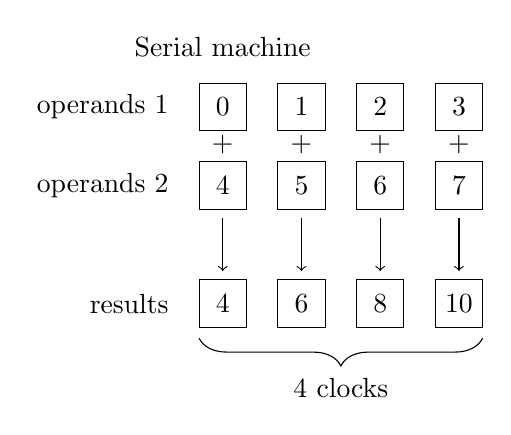
\begin{tikzpicture}
\foreach \x in {0,...,3}
{
	% Draw the rectangle 
	\draw (\x,0) rectangle (\x+.6,.6) node[pos=.5] (res\x) {
		\pgfmathparse{4+\x*2}
		\pgfmathprintnumber[precision=0]
        \pgfmathresult
    };
	\draw (\x,1.5) rectangle (\x+.6,2.1) node[pos=.5] (op2\x)  {
		\pgfmathparse{\x+4}
		\pgfmathprintnumber[precision=0]
        \pgfmathresult
    };
	\draw (\x,2.5) rectangle (\x+.6,3.1) node[pos=.5] (op1\x) {\x};
	% Draw the arrows for result
	\draw[->] ([yshift=-5pt]op2\x.south) -- ([yshift=5pt]res\x.north);
	\node at ([yshift=-7pt]op1\x.south) {$+$};
}
% add the arrow on top for clocks 
\draw [decorate,decoration={brace,amplitude=10pt,mirror,raise=4pt},yshift=0pt]
(0.,0) -- (3.6,0) node [black,midway,below,yshift=-15pt] {4 clocks};

\node[anchor=east] at ([xshift=-10pt]res0.west) {results};
\node[anchor=east] at ([xshift=-10pt]op10.west) {operands 1};
\node[anchor=east] at ([xshift=-10pt]op20.west) {operands 2};

\node[thick] at ([yshift=15pt]op10.north) {Serial machine};


% Add the name of architecture, classical serial 

% Add line name 
\end{tikzpicture}
\hspace{1cm}
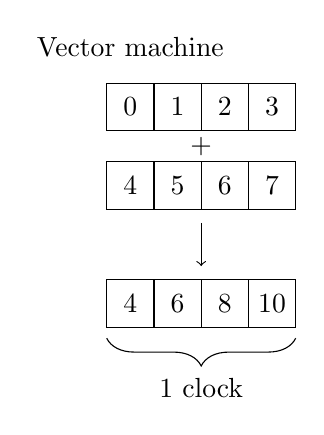
\begin{tikzpicture}
\foreach \x in {0,...,3}
{
	% Draw the rectangle 
	\draw (\x*.6,0) rectangle (\x*.6+.6,.6) node[pos=.5] (res\x) {
		\pgfmathparse{4+\x*2}
		\pgfmathprintnumber[precision=0]
        \pgfmathresult
    };
	\draw (\x*.6,1.5) rectangle (\x*.6+.6,2.1) node[pos=.5] (op2\x)  {
		\pgfmathparse{\x+4}
		\pgfmathprintnumber[precision=0]
        \pgfmathresult
    };
	\draw (\x*.6,2.5) rectangle (\x*.6+.6,3.1) node[pos=.5] (op1\x) {\x};
	% Draw the arrows for result
}

% Just onw arrow and plus sign 
\draw[->] ([yshift=-5pt]1.2,1.5) -- ([yshift=5pt]1.2,.6);
\node at ([yshift=-6pt]1.2,2.5) {$+$};

\draw [decorate,decoration={brace,amplitude=10pt,mirror,raise=4pt},yshift=0pt]
(0.,0) -- (2.4,0) node [black,midway,below,yshift=-15pt] {1 clock};

\node[thick] at ([yshift=15pt,]op10.north) {Vector machine};
\end{tikzpicture}
\end{center}
\caption{Vectorized processeur example on 4 integer addition: 128 bits wide bus}
\label{fig:2_HARD:vector}
\end{figure}

The behavior of vector machine is presented on figure~\ref{fig:2_HARD:vector} for a 16 bytes vector machine (4 integer of 4 bytes = 128 bits bus). 
We see on the left that performing the 4 operations requests in 4 cycle and, at the opposite, 1 cycle on the right with the vectorized machine.\\

Linked with the CPU optimizations, the memory optimizations also needs to be considered. 
Even if the ALU can perform billions of operations per second, it needs to be fed with data by fast transfers.

\subsubsection{Memory technology evolution}

The memories technologies optimizations address several aspects. 
The early 1980s saw the augmentation of bus size from 4 bits to presently 32 bits for single precision and 64 bits for double precision. 
Buses with 128 bits or 256 bits can also be used to allow vectorization presented just before. 

Different kind of technologies are considered in this study: the SRAM and DRAM. 

\paragraph{SRAM: }
\index{Static Random Access Memory}
The Static Random Access Memory (SRAM) is built using so called "flip-flop" circuits that can store data at any time time with no time lost in "refresh operations".
This kind of memory is very expensive to produce due to the number of transistors by memory cell, therefore, it is usually limited for small amounts of storage. 
The SRAM is mainly used for cache memory. 

\paragraph{DRAM: }
\index{Dynamic Random Access Memory}
The Dynamic Random Access Memory (DRAM) is based on transistors and capacitors to store binary information.
This memory is less expensive to produce but needs to be refreshed at a determined frequency, otherwise the data are lost. 
This refresh step is a read-write operation on the whole memory at a specific frequency. 
There are several sub-categories of DRAM used in different device depending on the way the bus are used with Single Data Rate (SDR), Double Data Rate (DDR) and Quad Data Rates (QDR). 
The number of data carried can vary from one times to four times, but the limitation of those products is the price and are constantly rising. 

The latest more efficient memory is the 3D memory.
This is a stack of the different components instead of usual 2D distribution.
This memory, 3D XPoint, was created by Intel and Micron Technology and announced in July 2015. 
It can now be find in the NVIDIA GPUs, named 3D-stacked in P100 and V100.

\subsubsection{Cache memory: }
\index{Cache mechanism}
\begin{figure}[t!]
\centering
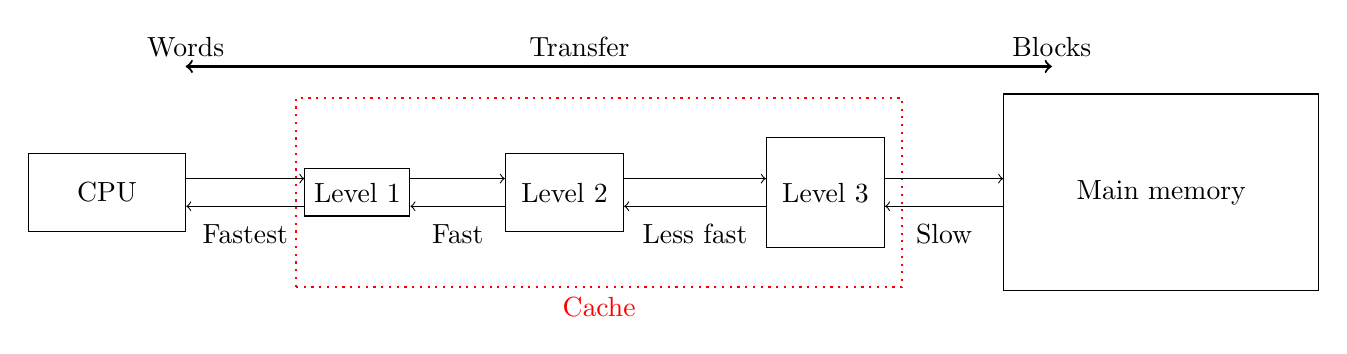
\begin{tikzpicture}
\node (rect) at (0,0) [draw,minimum width=2cm,minimum height=1cm] (cpu) {CPU};
\node[right = 1.5cm of cpu] (rect) [draw,minimum width=1cm,minimum height=.6cm] (cache_1) {Level 1};
\node[right = 1.2cm of cache_1] (rect) [draw,minimum width=1.5cm,minimum height=1cm] (cache_2) {Level 2};
\node[right = 1.8cm of cache_2] (rect) [draw,minimum width=1.5cm,minimum height=1.4cm] (cache_3) {Level 3};
\node[right = 1.5cm of cache_3] (rect) [draw,minimum width=4cm,minimum height=2.5cm] (ram) {Main memory};

\draw[thick,draw,red,dotted] (2.4,-1.2) rectangle  (10.1,1.2);
\node[below,red,thick] at (6.25,-1.2) {Cache}; 
% links 
\draw[->] ([yshift=5pt]cpu.east) -- ([yshift=5pt]cache_1.west);
\draw[<-] ([yshift=-5pt]cpu.east) -- ([yshift=-5pt]cache_1.west) node[midway,yshift=-10pt] {Fastest};

\draw[->] ([yshift=5pt]cache_1.east) -- ([yshift=5pt]cache_2.west);
\draw[<-] ([yshift=-5pt]cache_1.east) -- ([yshift=-5pt]cache_2.west) node[midway,yshift=-10pt] {Fast};

\draw[->] ([yshift=5pt]cache_2.east) -- ([yshift=5pt]cache_3.west);
\draw[<-] ([yshift=-5pt]cache_2.east) -- ([yshift=-5pt]cache_3.west) node[midway,yshift=-10pt] {Less fast};

\draw[->] ([yshift=5pt]cache_3.east) -- ([yshift=5pt]ram.west);
\draw[<-] ([yshift=-5pt]cache_3.east) -- ([yshift=-5pt]ram.west) node[midway,yshift=-10pt] {Slow};

\draw[<->,thick] (1,1.6) node[above]{Words} -- (12,1.6) node[above] {Blocks};
\node[above] at (6,1.6) {Transfer}; 
\end{tikzpicture}
\caption{Cache memory technology on three levels L1, L2 and L3}
\label{fig:2_HARD:caches}
\end{figure}
Cache is a memory mechanism that is useful to consider when targeting performance. 
The main idea of cache technology is presented on figure~\ref{fig:2_HARD:caches}.
This memory is built hierarchically over several levels. 
L1 is the closest to the CPU followed by L2 with generally no levels past L3 except on specific architectures. 
When looking for data, the CPU first checks if the data is present in the L1 cache, otherwise it will look in L2 and L3 to get the data to higher level. 
From the main memory to the L3 cache \textit{blocks} are exchanged, by chunks. 
With levels L1 and L2, lines of information are exchanged, usually referred to as \textit{words}.
This is based on the idea that if a data is used, it shall be used again in the near future.
Many cache architectures exist: direct, associative, fully associative, etc. 
Cache-hits occur when the data required is present in cache versus a cache-miss occurs when it has to be retrieved from lower levels or main memory. 
The ratio of cache-miss has to be kept low in a program in order to reach performance, and the impact may be very high.

\subsubsection{Pre-fetching} 
\index{Pre-fetching}
Pre-fecthing was developed based on memory optimization and especially for the cache.
When data are not available in L1 cache, it has to be moved from either L2 to L1 or L3 to L2 to L1 or in the worst case from RAM to L3 to L2 to L1. 
Pre-fecthing technology is a way to, knowing the next instructions operands, pre-fetch the data in closer cache before the instruction is decoded. 
The pre-fetch can either be hardware or software implemented and can concern data and even instructions.

\subsection{Multi-CPU servers and multi-core processors}
Around the beginning of the 2000s, the limitations of single core processors were very important. 
The frequency was already high and requested more power consumption causing more heat dissipation. 
The first solution to this problem was to provide multi-CPU devices, embedding several CPU on the same motherboard and allowing them to share memory. 
The evolution of the mono-core is the multi-core having several processing units on the same die allowed more optimization inside the die and combining all the advantages of single core processors.
But by embedding each CPU, the function and units required consume $n$ times more energy with cumulate heat effects.
Thus, unable to answer the constant augmentation of computational power needed for research and HPC, IBM was the first company to create a multi-core CPU in 2001, the Power4. 

Compared to the core inside multi-CPU, multi-core CPU shared one of the material (L3 caches, buses, etc.) and are implemented on the same due; this allows to reach the same CPU performances with less transistors and less power consumption, avoiding most of the heating issues. 

\begin{figure}
\centering 
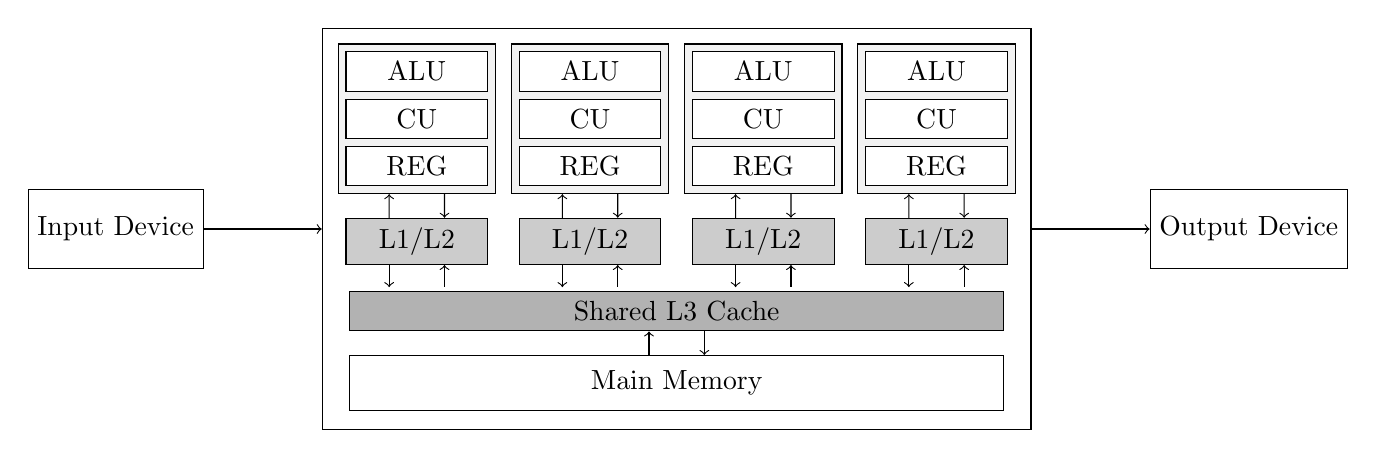
\begin{tikzpicture}

\node (rect) at (0,0) [draw,minimum width=2cm,minimum height=1cm] (input) {Input Device};

\node[right = 1.5cm of input] (rect) [draw,minimum width=9cm,minimum height=5.1cm] (machine) {};

\node[fill=black!30] (rect) at ([yshift=-3.6cm]machine.north) [draw,minimum width=8.3cm,minimum height=.5cm] (l3) {Shared L3 Cache};

\foreach \x in {0,...,3}{
	\node[anchor=north west,fill=black!5] (rect) at ([yshift=-.2cm,xshift=\x*2.2cm+.2cm]machine.north west) [draw,minimum width=2cm,minimum height=1.9cm] (cpu\x) {};

	\node[anchor=north west,fill=white] (rect) at ([yshift=-.1cm,xshift=.1cm]cpu\x.north west) [draw,minimum width=1.8cm,minimum height=.5cm] {ALU};
	\node[anchor=north west,fill=white] (rect) at ([yshift=-.7cm,xshift=.1cm]cpu\x.north west) [draw,minimum width=1.8cm,minimum height=.5cm] {CU};
	\node[anchor=north west,fill=white] (rect) at ([yshift=-1.3cm,xshift=.1cm]cpu\x.north west) [draw,minimum width=1.8cm,minimum height=.5cm] {REG};
	% Cache memory
	\node[anchor=north west,fill=black!20] (rect) at ([yshift=-.3cm,xshift=.1cm]cpu\x.south west) [draw,minimum width=1.8cm,minimum height=.5cm] (l1\x) {L1/L2};
	% Arriw 
	\draw[->] ([xshift=-10pt]l1\x.north) -- ([xshift=-10pt]cpu\x.south);
	\draw[<-] ([xshift=10pt]l1\x.north) -- ([xshift=10pt]cpu\x.south);
	% Arrow to L3
	\draw[->] ([xshift=-10pt]l1\x.south) -- ([xshift=-10pt,yshift=-8pt]l1\x.south);
	\draw[<-] ([xshift=10pt]l1\x.south) -- ([xshift=10pt,yshift=-8pt]l1\x.south);

	%\draw[<-] ([xshift=10pt]l1\x.south) |- (l3.north);
	
}


\node[below = .3cm of l3] (rect) [draw,minimum width=8.3cm,minimum height=.7cm] (mem) {Main Memory};

\node[right = 1.5cm of machine] (rect) [draw,minimum width=2cm,minimum height=1cm] (output) {Output Device};

\draw[->] ([xshift=-10pt]mem.north) -- ([xshift=-10pt]l3.south);
\draw[<-] ([xshift=10pt]mem.north) -- ([xshift=10pt]l3.south);

\draw[->] (input.east) -- (machine.west);
\draw[->] (machine.east) -- (output.west);

\end{tikzpicture}
\caption{Multi-core CPU with 4 cores based on Von Neumann Model}
\label{fig:2_HARD:von_neumann_model_multi-core}
\end{figure}

This architecture is presented on figure~\ref{fig:2_HARD:von_neumann_model_multi-core}.
The main memory is now shared between the cores. 
The registers and L1/L2 cache are the same but a L3 layer is added to the cache, and consistency has to be maintained over all the cores. 
If a process modifies a data in the memory this information has to be spread over all the other users of this data, even in their local cache. 

We note here that in current language the CPU, as describe in the Von Neumann model, is also the name of the die containing several cores. 
This is the architecture of most of current processors and these multi-cores provide two to 32 cores in most cases. 
Thus, the multi-core CPU are called "Host" and the attached accelerators are called "Devices".

\section{21th century architectures}
After years of development and research on hardware for Computer Science and specifically HPC, we present here the latest and best technologies to produce efficient and general-purpose supercomputers.

We present the latest architectures with multi-core, many-core and specific processors, and the most famous manufacturers. 

\subsection{Multi-core implementations}
The most world spread architecture in public and high performance computing is the multi-core processors. 
Most present-day accelerators require a classical processor to offload tasks and data on it. 

We start this presentation from the most popular processors in HPC world from the Intel company ones. 
We also present ARM which is a different multi-core architecture based on RISC instructions set.

\subsubsection{Intel}
\index{Intel}
Intel was created in 1968 by a chemist and a physicist, Gordon E. Moore and Robert Noyce, in Mountain View, California. 
Processors today are typically from Intel, the world leader which equips around 90\% of the supercomputers (November 2017 TOP500 list).

In 2007, Intel adopted a production model called the "Tick-Tock", presented on figure~\ref{fig:1_HPC:intel_tick_tock}.
\begin{figure}[t!]
\begin{center}
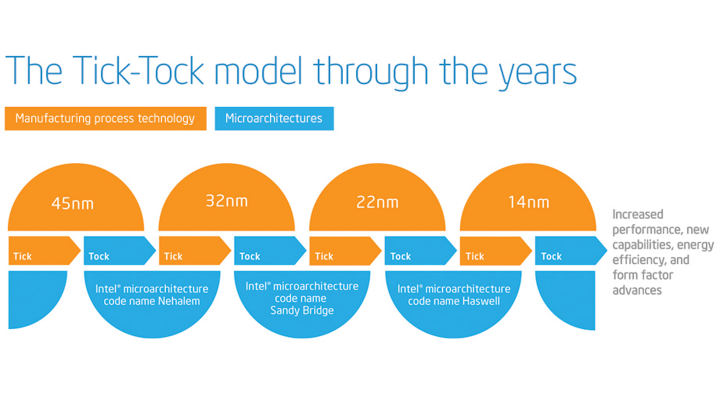
\includegraphics[width=.8\textwidth]{\locpath/figures/chap1/intel_tick_tock.png}
\caption{Intel Tick-Tock model}
\label{fig:1_HPC:intel_tick_tock}
\end{center}
\end{figure}
Since the creation of the Tick-Tock model, it always followed the same fashion: a new manufacturing technology, such as shrinking the chip with better engraving, on a "Tick" followed by a "Tock" which delivers a new micro-architecture.
The Intel processors for HPC are called Xeon and feature ECC memory, higher number of cores, large RAM support, large cache-memory, Hyper-threading, etc. 
Compared to desktop processors, their performances are of a different magnitude.
Intel has given every new processor a code name. 
The last generations are chronologically called Westemere (2011), Sandy Bridge (2012), Ivy Bridge(2013), Haswell (2014), Broadwell (2015), Skylake (2015) and Kaby lake (2016). 

Kaby Lake, the last architecture provided, does not exactly fit the typical "Tick-Tock" process because it is just based on optimizations of the Skylake architecture. 
The Kaby Lake is produced like Skylake with an engraving of 14 nm.
The Tick-Tock model appears to be hard to maintain due to the difficulties to engrave in less than 10 nm with quantum tunneling. 
This leads to using larger many-cores architecture and the bases of the next supercomputer evolutions, the road-map to hybrid models. 

\paragraph{Hyper-threading}
\index{Hyper-threading}
Another specificity of Intel Xeon processors is Hyper-threading (HT). 
This technology makes a single physical processing unit (core) appearing as two logical ones for the user's level.
In fact, a processor embedding 8 cores appears as a 16 cores for user. 
Adding more computation per node can technically allow the cores to switch context when data are fetched from the memory using the processor 100\% during all the computation. 
Multiple studies have been published on HT from Intel itself~\cite{marr2002hyperthreading} to independent researchers~\cite{bononi2006exploring,leng2002empirical}.
This optimization does not fit to all the cases of applications and can be disabled for normal use of the processors in the context of general purpose HPC architectures.

\subsubsection{ARM}
\index{Advanced RISC architecture}
Back in the 1980s, ARM stood for Acorn RISC Machine in reference to the first company to implement this kind of architecture, Acorn Computers. 
This company later changed the name to Advanced RISC Machine (ARM). 
ARM is a specific kind of processors based on RISC architecture as its ISA, despite usual processors using CISC.
The downside of CISC machines are they are difficult to create and they require way more transistor and thus more energy to work. 
The ISA from the RISC is simpler and requires multiple many transistors to operate and thus a smaller silicon area on the die.
Therefore, the energy required and the heat dissipated is less important. 
It becomes easier to create massively parallel processors based on ARM. 
On the other hand, simple ISA imposes more work on the source code compilation to fit the simple architecture. 
This makes the instructions sources longer, and therefore, more single instructions to execute. 

The ARM company provides several versions of ARM processors named Cortex-A7X (2015), Cortex-A5X (2014) and Cortex-A3X (2015) featured for highest-performances, for balancing performances and efficiency or for less power consumption, respectively. 

\index{Mont-Blanc project}
The new ARMv8 architecture starts to provide the tools to target HPC context~\cite{rico2017arm}.
The European approach towards energy efficient HPC, Mont-Blanc project\footnote{http://montblanc-project.eu/}, already constructs ARM based supercomputers. 
The exascale project in Horizon 2020 this project focuses on using ARM-based systems for HPC with many famous contributors, such as Atos/Bull as a project coordinator, ARM, French Alternative Energies and Atomic Energy Commission (CEA), Barcelona Supercomputing Center (BSC), etc.
The project is separated into several steps to finally reach Exascale near 2020. 
The last step, Mont-Blanc 3, is about to work on a pre-Exascale prototype powered by Cavium’s ThunderX2 ARM chip based on 64-bits ARMv8.

\subsection{Intel Xeon Phi}
\index{Xeon Phi}
Another specific HPC product from Intel is the Xeon Phi. 
This device can be considered as a Host or Device/Accelerator machine. 
Intel describes it as "a bootable host processor that delivers massive parallelism and vectorization".
This architecture embed multiple multi-cores processors interconnected and is called Intel's Many Integrated Core (MIC).
We placed this architecture here because it provides hundreds of conventional computation core but the program counter is not shared between them. 
It does not fit in the many-core architecture but is a step in the multi-core one. 
This is the technology on which Intel bases its Exascale machines. 

The architectures names are Knights Ferry, Knights Corner and Knight Landing~\cite{sodani2016knights}. 
The last architecture, Knight Hill, was recently canceled by Intel due to low performances and to focus the Xeon Phi for Exascale.
The main advantage of this architecture compared to GPGPUs is the x86 compatibility of the embedded cores and the fact this device can boot and use to drive other accelerators. 
They also feature more complex operations and handle double precision natively.

\subsection{Many-core architecture, SIMT execution model}
\index{Single Instruction Multiple Threads}
Several architectures can be defined as many-cores and follow the SIMD model from Flynn taxonomy.
These devices integrate thousands of cores that are usually control by fewer control units. 
We can consider these cores as "simpler" since they have to work synchronously and under the coordination of a control unit.
Some devices are specific like the Xeon Phi of Intel, integrating a hundred of regular processor cores which can work independently. 

\subsubsection{GPU}
\index{Graphics Processing Unit}
A CPU can usually have two to 32 computation cores that can operate on different instruction streams, but the SIMT architecture of the GPU is slightly different. 
The cores are grouped and must share the same instruction at the same clock time, but different groups can have their own instructions. 

\begin{figure}
\begin{center}
% classical processor
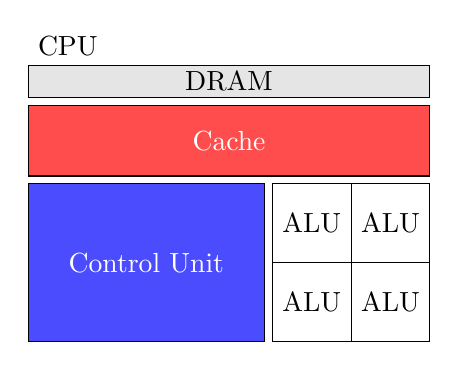
\begin{tikzpicture}
% ALUs
\foreach \x in {3,...,4}
	\foreach \y in {0,...,1}
		\draw[] (\x+.1,\y) rectangle (\x+1.1,\y+1) node[pos=.5] {ALU};
% Control Unit
\draw[fill=blue!70] (0,0) rectangle (3,2) node[pos=.5,text=white] {Control Unit};
%Cache
\draw[fill=red!70] (0,2.1) rectangle (5.1,3) node[pos=.5,text=white] {Cache};
% DRAM
\draw[fill=black!10] (0,3.1) rectangle (5.1,3.5) node[pos=.5] {DRAM};
%Name 
\node[yshift=7pt,anchor=west] at (0,3.5) {CPU};
\end{tikzpicture}
\hspace{1cm}
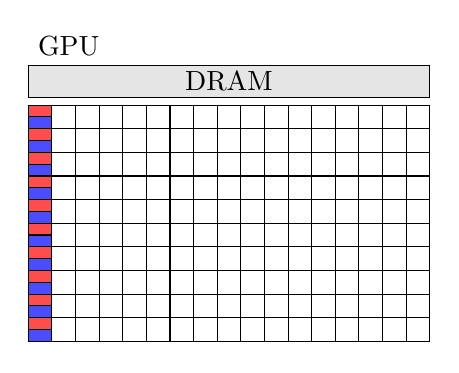
\begin{tikzpicture}
% ALUs
\foreach \y in {0,...,9}
{
	\draw[fill=blue!70] (0,\y * .3) rectangle (.3,\y * .3 + .15) node[pos=.5] {};
	\draw[fill=red!70] (0,\y * .3 + .15) rectangle (.3,\y * .3 + .3) node[pos=.5] {};
	\foreach \x in {1,...,16}
		\draw[] (\x*.3,\y*.3) rectangle (\x *.3+.3,\y*.3+.3) node[pos=.5] {};
}
% DRAM
\draw[fill=black!10] (0,3.1) rectangle (5.1,3.5) node[pos=.5] {DRAM};
% Name 
\node[yshift=7pt,anchor=west] at (0,3.5) {GPU};
\end{tikzpicture}
\end{center}
\caption{Multi-core versus Many-core architecture, case of GPUs}
\label{fig:2_HARD:gpu}
\end{figure}

Figure~\ref{fig:2_HARD:gpu} present the vision between CPU and GPU processors. 
We note in this figure that the usual topology with the ALU lined up in front of their control unit and shared cache memory. 
Every ALU has its own memory and registers to operate local computations. 

These devices are called General Purpose Graphics Processing Units (GPGPUs). 
They are derivative from classical GPUs used for graphical purpose.
Pioneers show that GPGPUs can be use efficiently for classical scientific computations.
The vendor provides then specific GPU for general purpose computing.  
We present here the two main companies providing GPGPUs for HPC world: NVIDIA and AMD.

\paragraph{NVIDIA GPU architecture}
\index{NVIDIA}
The NVIDIA company was founded in April 1993 in Santa Clara, Carolina by three persons, one being the current CEO, Jensen Huang.
The company name originated from \textit{invidia} the Latin word for Envy and vision for graphical rendering. 

NVIDIA is known as the pioneer in graphics, cryptocurrency, portable devices, and now Artificial Intelligence (IA) and appears to be even the creator of the name "GPU".
NVIDIA's GPUs, inspired from visualization and gaming at a first glance, are available as a dedicated device for HPC purpose since the company released the brand named \textit{Tesla}. 
The public GPUs can also be used for dedicated computation, but does not feature ECC memory, double precision or special functions/FFT cores. 
The different versions of the architecture are named following famous physicists, chronologically: Tesla, Fermi, Kepler, Maxwell, Pascal and Volta.

\index{K20Xm}
We describe here the Kepler brand GPU and more specifically the K20Xm GPU on which we based our study. 
\begin{figure}
\centering
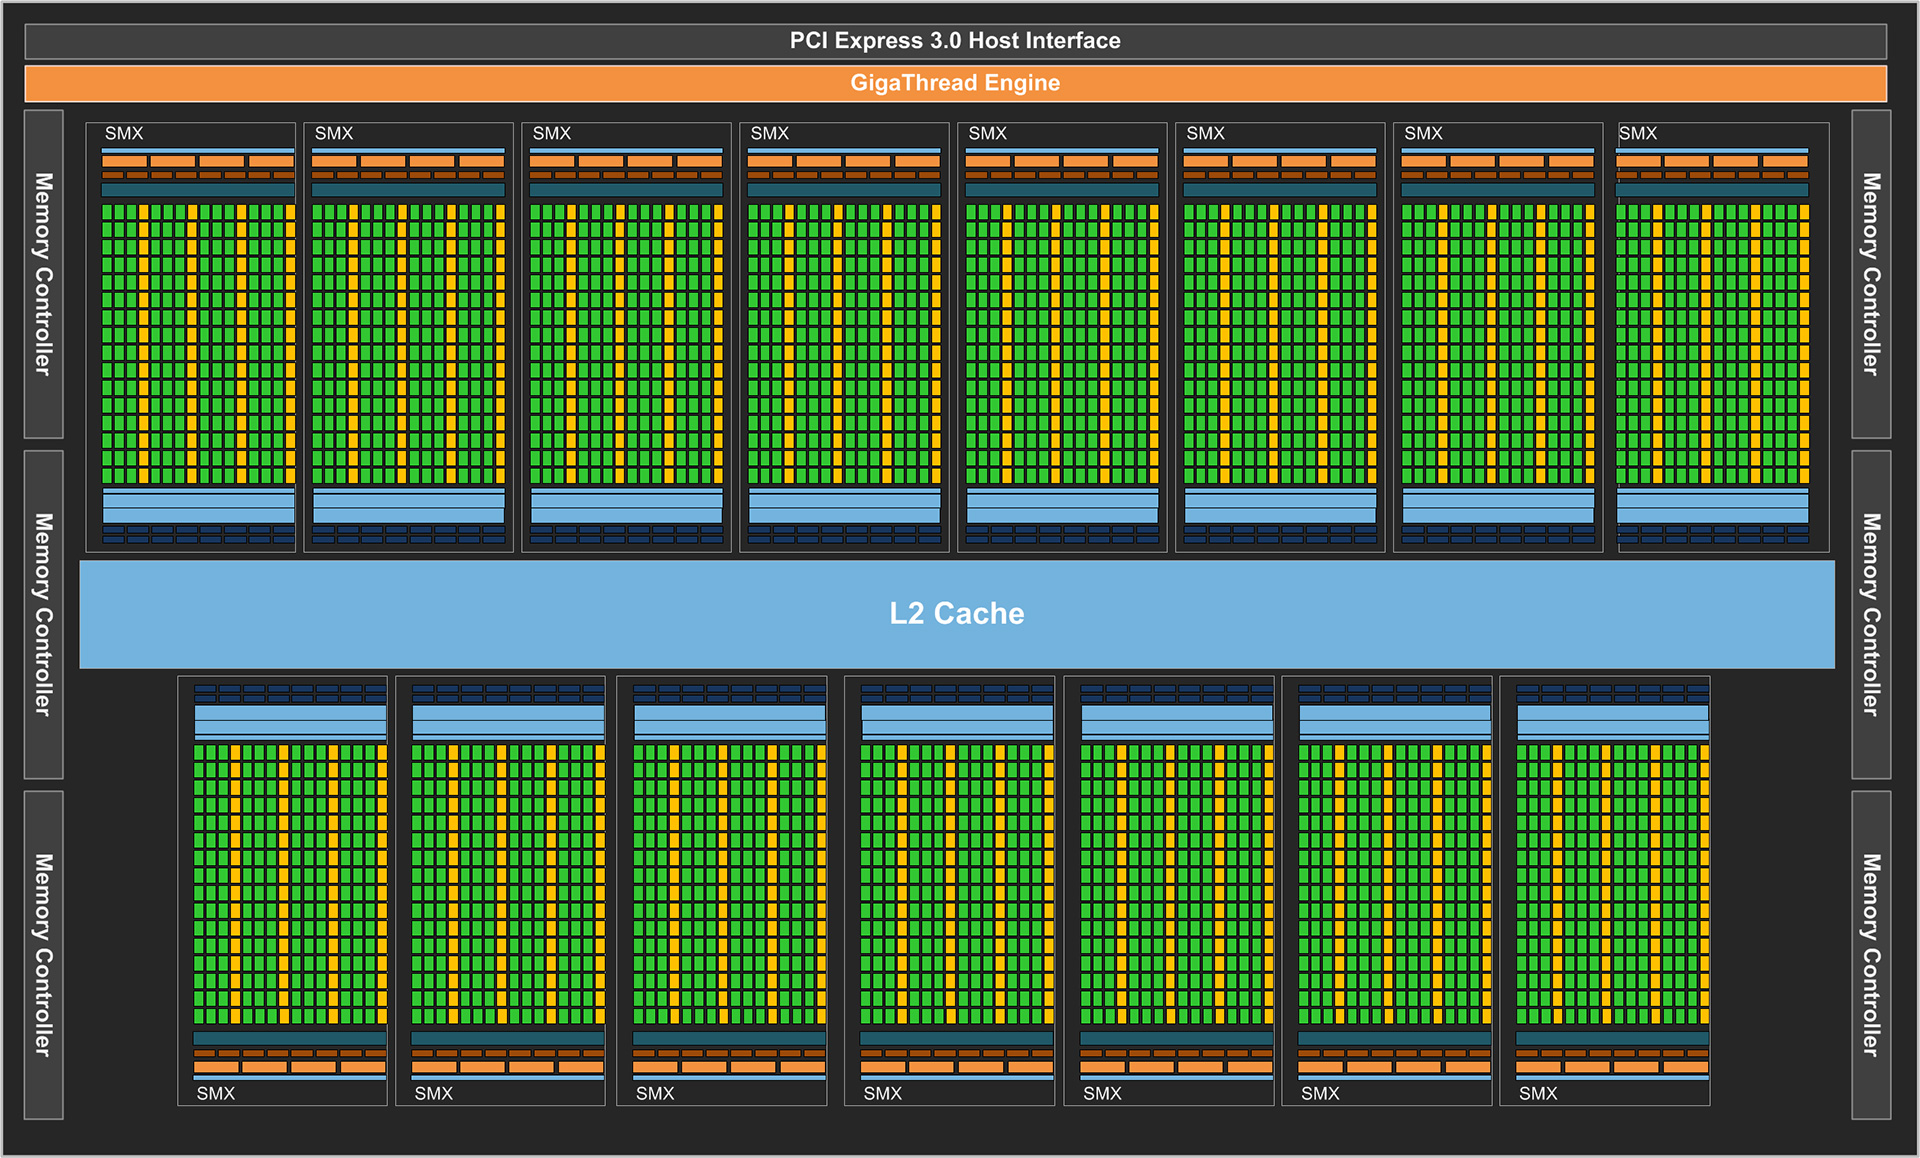
\includegraphics[width=\textwidth]{\locpath/figures/chap1/kepler_architecture.jpeg}
\caption{NVIDIA Tesla Kepler architecture. Single-precision in green and double-precision in yellow}
\label{fig:2_HARD:kepler_arch}
\end{figure}
This NVIDIA Tesla Kepler GPU is based on the GK110 graphics processor describes in the white-paper\cite{nvidia2012nvidias} on 28nm process.
The figure~\ref{fig:2_HARD:kepler_arch} is a representation of the physical elements of this graphics processor. 
The K20X comes in active and passive cooling mode with K20Xc and K20Xm, respectively.
This GPU embeds 2688 CUDA cores distributed in 14 SMX (we note that GK110 normally provides 15 SMX but only 14 are present on the K20X).
In this model each SMX contains 192 single precisions cores, 64 double precision cores, 32 special function units and 32 load/store units.
In a SMX the memory provides 65536 32-bits registers, 64 KB of shared memory L1 cache, 48 KB of read-only cache
The L2 cache is 1546 KB shared by the SMX for a total of 6 GB of memory adding the DRAM.
The whole memory is protected using Single‐Error Correct Double‐Error Detect (SECDED) ECC code.
The power consumption is estimated to 225 W.
This GPGPU is expected to produce 1.31 TFLOPS for double-precision and 3.95 TFLOPS of single-precision.

\paragraph{AMD}
\index{AMD}
Another company is providing GPUs for HPC, Advanced Micro Devices (AMD). 
In front of the huge success of NVIDIA GPU that leads from far the HPC market, it is hard for AMD to find a place for its GPGPUs, the FirePro, in HPC. 
The FirePro is targeted using a language near CUDA, not held by a single company by NVIDIA like CUDA, called OpenCL. 
An interesting creation of AMD is the Accelerated Processing Units (APUs) which embedded the processor and the GPU on the same die since 2011. 
This solution allows them to target the same memory. 

In the race to market and performances, AMD found an accord with Intel to provide dies featuring Intel processor, AMD GPU and common HBM memory. 
The project is call Kaby Lake-G and announced it would be available in the first semester of 2018 for public, not HPC itself. 

\subsubsection{PEZY}
\index{PEZY}
Another many-core architecture only appeared in the last benchmarks. 
The PEZY Super Computer 2, PEZY-SC2, is the third many-core microprocessor developed by the company PEZY. 
The three first machines ranked in the GREEN500 list are accelerator using this many-core die. 
We also note that in the November 2017 list, the fourth supercomputer, Gyoukou, is also powered by PEZY-SC2 cards.

\subsection{Other architectures}
Numerous architectures have not been presented here because they are out of scope of this study. 
We present here two technologies we have encountered in our researches and that may be tomorrow solution for Exascale in HPC. 
\subsubsection{FPGA}
\index{Field Programmable Gates Array}
Field Programmable Gates Array (FPGA) are devices that can be reprogram to fit the needs of the user after their construction.
The leader were historically Altera with the Stratix, Arria and Cyclone FPGAs, which is now part of Intel. 
With the FPGAs, the users have access to the hardware and can design their own circuits. 
Currently, FPGA can be targeted with OpenCL programming language. 
The arrival of Intel in this market assures the best hopes for HPC version of FPGAs. 
The main gap for users is the circuit building that can be designed for specific needs but may be hard to setup. 
\subsubsection{ASIC}
\index{Application Specified Integrated Circuits}
Application Specified Integrated Circuits are dedicated device construct for on purpose. 
An example of ASIC is the Gravity Pipe (GRAPE) which is dedicated to compute gravitation given mass and positions.
Google leads the way for ASIC and recently created its dedicated devices to boost AI bots.
ASIC may be found in some optimized communication devices, such as fast interconnection network in HPC.  

\section{Distributed architectures}

The technologies presented in previous part is the milestone of supercomputers. 
They are used together in a whole system to create machine delivering incredible computational power.

\subsection{Architecture of a supercomputer}
From the hardware described before, we can create the architecture of a cluster from the smallest unit, cores, nodes, to the whole system.

\begin{description}[noitemsep,nolistsep]
\item[Core:] A core is the smallest unit in our devices. 
It refers to the Von Neumann model in case of core with ALU and CU. 
We can separate cores from CPU to GPU, the first one able to be independent whereas the second ones working together and share the same program counter. 
\item[Socket/Host:] A socket is mistakenly called a CPU in current language. 
It is, for multi-cores sockets, composed of several cores. 
The name Host comes from the Host-Device architecture using accelerators. 
\item[Accelerators/Devices:] Accelerators are devices that, when attached to the Host, provide additional computational power. 
We can identify them as GPUs, FPGAs, ASICs, etc. 
A socket can have access to one or more accelerators and can also share the accelerator usage. 
\item[Computation node: ] The next layer of our HPC system is the computation node, which is a group of several sockets and accelerators sharing memory;
\item[Rack: ] A rack is a set of computation nodes, generally in vertical stack. 
It may also include specific nodes dedicated to the network or the Input/Output.
\item[Interconnection: ] The nodes are grouped together with hard wire connection following a specific interconnection topology with very high bandwidth.
\item[System/Cluster/Supercomputer] The cluster group several racks though an interconnection network.
\end{description}

An interconnect technology is required in order to connect nodes together and allow distributed programming. 
Interconnection networks are the way the nodes of a cluster are connected together. 

\subsection{Interconnection topologies}
\index{Interconnect}
Several topologies exist from point to point to multi-dimensional torus.
%
\begin{figure}[t!]
\centering
\resizebox {.14\columnwidth} {!} {
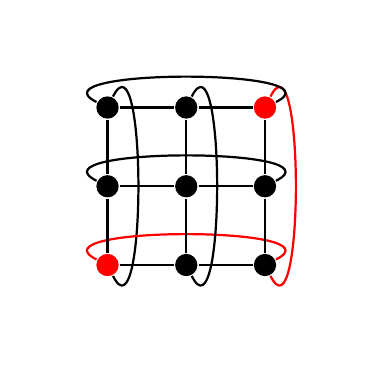
\begin{tikzpicture}[thick,inner sep=0.1cm]
	\node [fill,circle,red] (node 1000) at (0,0) {};
	\node [fill,circle] (node 1001) at (1,0) {};
	\node [fill,circle] (node 1002) at (2,0) {};
	\node [fill,circle] (node 1003) at (0,1) {};
	\node [fill,circle] (node 1004) at (1,1) {};
	\node [fill,circle] (node 1005) at (2,1) {};
	\node [fill,circle] (node 1006) at (0,2) {};
	\node [fill,circle] (node 1007) at (1,2) {};
	\node [fill,circle,red] (node 1008) at (2,2) {};
	
	\draw (node 1000)
							         .. controls +(0.500000,-1.000000)
							                 and +(0.500000,1.000000)
							         .. (node 1006);
	\draw[red] (node 1000)
							         .. controls +(-1.000000,0.500000)
							                 and +(1.000000,0.500000)
							         .. (node 1002);
	\draw (node 1000) -- (node 1001);
	\draw (node 1000) -- (node 1003);
	\draw (node 1001) -- (node 1004);
	\draw (node 1001)
							         .. controls +(0.500000,-1.000000)
							                 and +(0.500000,1.000000)
							         .. (node 1007);
	\draw (node 1002) -- (node 1005);
	\draw (node 1002) -- (node 1001);
	\draw[red] (node 1002)
							         .. controls +(0.500000,-1.000000)
							                 and +(0.500000,1.000000)
							         .. (node 1008);
	
	\draw (node 1003)
							         .. controls +(-1.000000,0.500000)
							                 and +(1.000000,0.500000)
							         .. (node 1005);
	\draw (node 1003) -- (node 1006);
	\draw (node 1003) -- (node 1004);
	\draw (node 1004) -- (node 1005);
	\draw (node 1004) -- (node 1007);
	\draw (node 1005) -- (node 1008);
	\draw (node 1006)
							         .. controls +(-1.000000,0.500000)
							                 and +(1.000000,0.500000)
							         .. (node 1008);
	\draw (node 1006) -- (node 1007);
	\draw (node 1007) -- (node 1008);
\end{tikzpicture}
}
%\vspace{1cm}
\resizebox {.34\columnwidth} {!} {
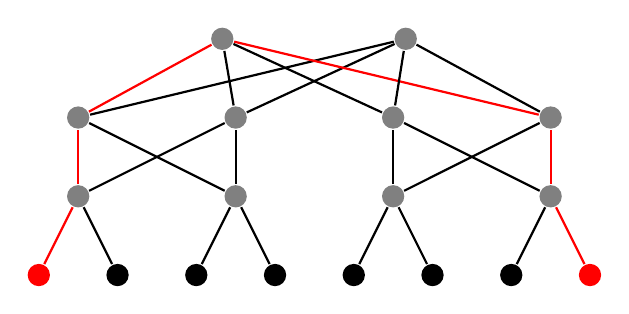
\begin{tikzpicture}[thick,inner sep=0.1cm]
	
	\node [fill,circle,red] (node a) at (0,0) {};
	\node [fill,circle] (node b) at (1,0) {};
	\node [fill,circle] (node c) at (2,0) {};
	\node [fill,circle] (node d) at (3,0) {};
	\node [fill,circle] (node e) at (4,0) {};
	\node [fill,circle] (node f) at (5,0) {};
	\node [fill,circle] (node g) at (6,0) {};
	\node [fill,circle,red] (node h) at (7,0) {};

	\node [fill,circle,black!50] (node a0) at (0.5,1) {};
	\node [fill,circle,black!50] (node a1) at (2.5,1) {};
	\node [fill,circle,black!50] (node a2) at (4.5,1) {};
	\node [fill,circle,black!50] (node a3) at (6.5,1) {};
	\node [fill,circle,black!50] (node a4) at (0.5,2) {};
	\node [fill,circle,black!50] (node a5) at (2.5,2) {};
	\node [fill,circle,black!50] (node a6) at (4.5,2) {};
	\node [fill,circle,black!50] (node a7) at (6.5,2) {};

	\node [fill,circle,black!50] (node n0) at (2.33,3) {};
	\node [fill,circle,black!50] (node n1) at (4.66,3) {};

	\draw[red] (node a) -- (node a0);
	\draw (node b) -- (node a0);
	\draw (node c) -- (node a1);
	\draw (node d) -- (node a1);
	\draw (node e) -- (node a2);
	\draw (node f) -- (node a2);
	\draw (node g) -- (node a3);
	\draw[red] (node h) -- (node a3);

	\draw[red] (node a0) -- (node a4);
	\draw (node a0) -- (node a5);
	\draw (node a1) -- (node a4);
	\draw (node a1) -- (node a5);
	\draw (node a2) -- (node a6);
	\draw (node a2) -- (node a7);
	\draw (node a3) -- (node a6);
	\draw[red] (node a3) -- (node a7);

	\draw[red] (node n0) -- (node a4);
	\draw (node n1) -- (node a5);
	\draw (node n0) -- (node a5);
	\draw (node n1) -- (node a4);
	\draw (node n0) -- (node a6);
	\draw (node n1) -- (node a7);
	\draw[red] (node n0) -- (node a7);
	\draw (node n1) -- (node a6);
\end{tikzpicture}
}
%\caption{Torus and 4-ary tree}
%\end{figure}
%\begin{figure}
\resizebox {.24\columnwidth} {!} {
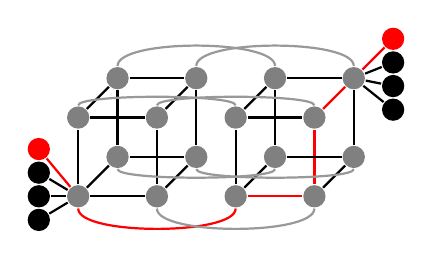
\begin{tikzpicture}[thick,inner sep=0.1cm]
	
	\node [fill,circle,black!50] (node a0) at (0,0) {};
	\node [fill,circle,black!50] (node b0) at (1,0) {};
	\node [fill,circle,black!50] (node c0) at (0,1) {};
	\node [fill,circle,black!50] (node d0) at (1,1) {};
	\node [fill,circle,black!50] (node e0) at (0.5,0.5) {};
	\node [fill,circle,black!50] (node f0) at (1.5,0.5) {};
	\node [fill,circle,black!50] (node g0) at (0.5,1.5) {};
	\node [fill,circle,black!50] (node h0) at (1.5,1.5) {};

	\node [fill,circle,black!50] (node a1) at (2,0) {};
	\node [fill,circle,black!50] (node b1) at (3,0) {};
	\node [fill,circle,black!50] (node c1) at (2,1) {};
	\node [fill,circle,black!50] (node d1) at (3,1) {};
	\node [fill,circle,black!50] (node e1) at (2.5,0.5) {};
	\node [fill,circle,black!50] (node f1) at (3.5,0.5) {};
	\node [fill,circle,black!50] (node g1) at (2.5,1.5) {};
	\node [fill,circle,black!50] (node h1) at (3.5,1.5) {};

	\node [fill,circle,red] (node cn0) at (4,2.) {};
	\node [fill,circle] (node cn1) at (4,1.7) {};
	\node [fill,circle] (node cn2) at (4,1.4) {};
	\node [fill,circle] (node cn3) at (4,1.1) {};

	\node [fill,circle] (node cn4) at (-0.5,-0.3) {};
	\node [fill,circle] (node cn5) at (-0.5,0.0) {};
	\node [fill,circle] (node cn6) at (-0.5,0.3) {};
	\node [fill,circle,red] (node cn7) at (-0.5,0.6) {};


	\draw (node a0) -- (node b0);
	\draw (node b0) -- (node d0);
	\draw (node c0) -- (node d0);
	\draw (node a0) -- (node c0);
	\draw (node e0) -- (node f0);
	\draw (node f0) -- (node h0);
	\draw (node g0) -- (node h0);
	\draw (node e0) -- (node g0);

	\draw (node a0) -- (node e0);
	\draw (node b0) -- (node f0);
	\draw (node c0) -- (node g0);
	\draw (node d0) -- (node h0);

	\draw[red] (node a1) -- (node b1);
	\draw[red] (node b1) -- (node d1);
	\draw (node c1) -- (node d1);
	\draw (node a1) -- (node c1);
	\draw (node e1) -- (node f1);
	\draw (node f1) -- (node h1);
	\draw (node g1) -- (node h1);
	\draw (node e1) -- (node g1);

	\draw (node a1) -- (node e1);
	\draw (node b1) -- (node f1);
	\draw (node c1) -- (node g1);
	\draw[red] (node d1) -- (node h1);

	\draw[red] (node cn0) -- (node h1);
	\draw (node cn1) -- (node h1);
	\draw (node cn2) -- (node h1);
	\draw (node cn3) -- (node h1);
	\draw (node cn4) -- (node a0);
	\draw (node cn5) -- (node a0);
	\draw (node cn6) -- (node a0);
	\draw[red] (node cn7) -- (node a0);

	%\draw (node a0) -- (node a1);
	\draw[red] (node a0)
		        .. controls +(0.,-0.500000)
		                 and +(0.,-0.500000)
		        .. (node a1);
	\draw[black!40] (node b0) 
				.. controls +(0.,-0.500000)
		                 and +(0.,-0.500000)
		        .. (node b1);
	\draw[black!40] (node c0) 
				.. controls +(0.,0.300000)
		                 and +(0.,0.300000)
		        ..  (node c1);
	\draw[black!40] (node d0) 
				.. controls +(0.,0.300000)
		                 and +(0.,0.300000)
		        ..  (node d1);
	\draw[black!40] (node e0) 
				.. controls +(0.,-0.300000)
		                 and +(0.,-0.300000)
		        ..  (node e1);
	\draw[black!40] (node f0) 
				.. controls +(0.,-0.300000)
		                 and +(0.,-0.300000)
		        ..  (node f1);
	\draw[black!40] (node g0) 
				.. controls +(0.,0.500000)
		                 and +(0.,0.500000)
		        ..  (node g1);
	\draw[black!40] (node h0) 
				.. controls +(0.,0.500000)
		                 and +(0.,0.500000)
		        ..  (node h1);
\end{tikzpicture}
}
%\hspace{1cm}
\resizebox {.24\columnwidth} {!} {
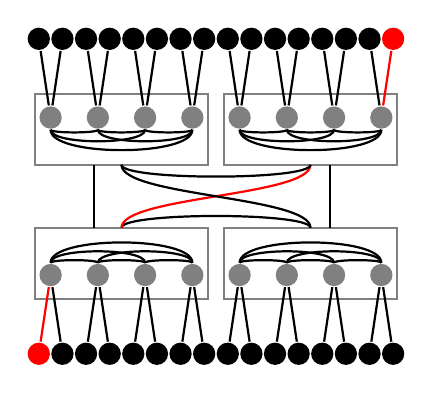
\begin{tikzpicture}[thick,inner sep=0.1cm]
	\node [fill,circle,black!50] (node a00) at (0.45,1) {};
	\node [fill,circle,black!50] (node a01) at (1.05,1) {};
	\node [fill,circle,black!50] (node a02) at (1.65,1) {};
	\node [fill,circle,black!50] (node a03) at (2.25,1) {};
	\node [fill,circle,red] (node n01) at (0.3,0) {};
	\node [fill,circle] (node n02) at (0.6,0) {};
	\node [fill,circle] (node n03) at (0.9,0) {};
	\node [fill,circle] (node n04) at (1.2,0) {};
	\node [fill,circle] (node n05) at (1.5,0) {};
	\node [fill,circle] (node n06) at (1.8,0) {};
	\node [fill,circle] (node n07) at (2.1,0) {};
	\node [fill,circle] (node n08) at (2.4,0) {};

	\node [fill,circle,black!50] (node a10) at (2.85,1) {};
	\node [fill,circle,black!50] (node a11) at (3.45,1) {};
	\node [fill,circle,black!50] (node a12) at (4.05,1) {};
	\node [fill,circle,black!50] (node a13) at (4.65,1) {};
	\node [fill,circle] (node n11) at (2.7,0) {};
	\node [fill,circle] (node n12) at (3,0) {};
	\node [fill,circle] (node n13) at (3.3,0) {};
	\node [fill,circle] (node n14) at (3.6,0) {};
	\node [fill,circle] (node n15) at (3.9,0) {};
	\node [fill,circle] (node n16) at (4.2,0) {};
	\node [fill,circle] (node n17) at (4.5,0) {};
	\node [fill,circle] (node n18) at (4.8,0) {};

	\node [fill,circle,black!50] (node a20) at (0.45,3) {};
	\node [fill,circle,black!50] (node a21) at (1.05,3) {};
	\node [fill,circle,black!50] (node a22) at (1.65,3) {};
	\node [fill,circle,black!50] (node a23) at (2.25,3) {};
	\node [fill,circle] (node n21) at (0.3,4) {};
	\node [fill,circle] (node n22) at (0.6,4) {};
	\node [fill,circle] (node n23) at (0.9,4) {};
	\node [fill,circle] (node n24) at (1.2,4) {};
	\node [fill,circle] (node n25) at (1.5,4) {};
	\node [fill,circle] (node n26) at (1.8,4) {};
	\node [fill,circle] (node n27) at (2.1,4) {};
	\node [fill,circle] (node n28) at (2.4,4) {};

	\node [fill,circle,black!50] (node a30) at (2.85,3) {};
	\node [fill,circle,black!50] (node a31) at (3.45,3) {};
	\node [fill,circle,black!50] (node a32) at (4.05,3) {};
	\node [fill,circle,black!50] (node a33) at (4.65,3) {};
	\node [fill,circle] (node n31) at (2.7,4) {};
	\node [fill,circle] (node n32) at (3,4) {};
	\node [fill,circle] (node n33) at (3.3,4) {};
	\node [fill,circle] (node n34) at (3.6,4) {};
	\node [fill,circle] (node n35) at (3.9,4) {};
	\node [fill,circle] (node n36) at (4.2,4) {};
	\node [fill,circle] (node n37) at (4.5,4) {};
	\node [fill,circle,red] (node n38) at (4.8,4) {};

	\draw[black!50] (2.65,2.4) rectangle (4.85,3.3);
	\draw[black!50] (0.25,2.4) rectangle (2.45,3.3);

	\draw[black!50] (2.65,0.7) rectangle (4.85,1.6);
	\draw[black!50] (0.25,0.7) rectangle (2.45,1.6);

	\draw (1.35,1.6)
	.. controls +(0.,0.2)
	    and +(0.,0.2)
	..  (3.75,1.6); 

	\draw[red] (1.35,1.6)
	.. controls +(0.,0.4)
	    and +(0.,-0.4)
	..  (3.75,2.4); 
	%\draw (1.35,1.6) -- (3.75,2.4);
	\draw (3.75,1.6)
	.. controls +(0.,0.4)
	    and +(0.,-0.4)
	..  (1.35,2.4); 
	%\draw (3.75,1.6) -- (1.35,2.4);

	\draw (1.,1.6) -- (1.,2.4);
	\draw (4.,1.6) -- (4.,2.4);

	\draw (1.35,2.4)
	.. controls +(0.,-0.2)
	    and +(0.,-0.2)
	..  (3.75,2.4); 


	\draw[red] (node n01) -- (node a00);
	\draw (node n02) -- (node a00);
	\draw (node n03) -- (node a01);
	\draw (node n04) -- (node a01);
	\draw (node n05) -- (node a02);
	\draw (node n06) -- (node a02);
	\draw (node n07) -- (node a03);
	\draw (node n08) -- (node a03);

	\draw (node n11) -- (node a10);
	\draw (node n12) -- (node a10);
	\draw (node n13) -- (node a11);
	\draw (node n14) -- (node a11);
	\draw (node n15) -- (node a12);
	\draw (node n16) -- (node a12);
	\draw (node n17) -- (node a13);
	\draw (node n18) -- (node a13);

	\draw (node n21) -- (node a20);
	\draw (node n22) -- (node a20);
	\draw (node n23) -- (node a21);
	\draw (node n24) -- (node a21);
	\draw (node n25) -- (node a22);
	\draw (node n26) -- (node a22);
	\draw (node n27) -- (node a23);
	\draw (node n28) -- (node a23);

	\draw (node n31) -- (node a30);
	\draw (node n32) -- (node a30);
	\draw (node n33) -- (node a31);
	\draw (node n34) -- (node a31);
	\draw (node n35) -- (node a32);
	\draw (node n36) -- (node a32);
	\draw (node n37) -- (node a33);
	\draw[red] (node n38) -- (node a33);

	\draw (node a00) 
	.. controls +(0.,0.2)
	    and +(0.,0.2)
	..  (node a01);
	\draw (node a00) 
	.. controls +(0.,0.35)
	    and +(0.,0.35)
	..  (node a02);
	\draw (node a00) 
	.. controls +(0.,0.5)
	    and +(0.,0.5)
	..  (node a03);
	\draw (node a01) 
	.. controls +(0.,0.2)
	    and +(0.,0.2)
	..  (node a02);
	\draw (node a01) 
	.. controls +(0.,0.35)
	    and +(0.,0.35)
	..  (node a03);
	\draw (node a02) 
	.. controls +(0.,0.2)
	    and +(0.,0.2)
	..  (node a03);

	\draw (node a10) 
	.. controls +(0.,0.2)
	    and +(0.,0.2)
	..  (node a11);
	\draw (node a10) 
	.. controls +(0.,0.35)
	    and +(0.,0.35)
	..  (node a12);
	\draw (node a10) 
	.. controls +(0.,0.5)
	    and +(0.,0.5)
	..  (node a13);
	\draw (node a11) 
	.. controls +(0.,0.2)
	    and +(0.,0.2)
	..  (node a12);
	\draw (node a11) 
	.. controls +(0.,0.35)
	    and +(0.,0.35)
	..  (node a13);
	\draw (node a12) 
	.. controls +(0.,0.2)
	    and +(0.,0.2)
	..  (node a13);

	\draw (node a20) 
	.. controls +(0.,-0.2)
	    and +(0.,-0.2)
	..  (node a21);
	\draw (node a20) 
	.. controls +(0.,-0.35)
	    and +(0.,-0.35)
	..  (node a22);
	\draw (node a20) 
	.. controls +(0.,-0.5)
	    and +(0.,-0.5)
	..  (node a23);
	\draw (node a21) 
	.. controls +(0.,-0.2)
	    and +(0.,-0.2)
	..  (node a22);
	\draw (node a21) 
	.. controls +(0.,-0.35)
	    and +(0.,-0.35)
	..  (node a23);
	\draw (node a22) 
	.. controls +(0.,-0.2)
	    and +(0.,-0.2)
	..  (node a23);

	\draw (node a30) 
	.. controls +(0.,-0.2)
	    and +(0.,-0.2)
	..  (node a31);
	\draw (node a30) 
	.. controls +(0.,-0.35)
	    and +(0.,-0.35)
	..  (node a32);
	\draw (node a30) 
	.. controls +(0.,-0.5)
	    and +(0.,-0.5)
	..  (node a33);
	\draw (node a31) 
	.. controls +(0.,-0.2)
	    and +(0.,-0.2)
	..  (node a32);
	\draw (node a31) 
	.. controls +(0.,-0.35)
	    and +(0.,-0.35)
	..  (node a33);
	\draw (node a32) 
	.. controls +(0.,-0.2)
	    and +(0.,-0.2)
	..  (node a33);
\end{tikzpicture}
}
\caption{Torus, Fat-Tree, HyperX, DragonFly}
\label{fig:1_HPC:topology}
\end{figure}
%
The figure~\ref{fig:1_HPC:topology} is a representation of famous topologies. 
Each interconnect technology has its own specificity. 
These networks take in account the number of nodes to interconnect and the targeted bandwidth/budget.
Several declination of each network are not detailed here. 
The Mesh and the Torus are used as a basis in lower layers of others more complex interconnection networks. 
A perfect example is the supercomputer called K-Computer describe in the next section.
The Fat Tree presented here is a k-ary Fat Tree, the higher the position in the tree, the more connections are found and with a bandwidth being important. 
The nodes are available as the leaves, on the middle level we find the switches and on top the routers. 
This is the topology of the ROMEO supercomputer we used for our tests. 
Another topology, HyperX\cite{ahn2009hyperx}, is based on Hyper-Cube.
The DragonFly\cite{kim2008technology} interconnect is recent, 2008, and is used in modern day supercomputers.

InfiniBand (IB)\index{Infiniband} is the most widespread technology used for interconnection with different kind of bandwidth presented in figure~\ref{fig:1_HPC:infiniband}.
It provides high bandwidth and small latency and companies such as Intel, Mellanox, etc. provide directly adapters and switches specifically for IB. 

\begin{table}[t!]
\begin{center}
\[\arraycolsep=0.pt\def\arraystretch{1.2}
\begin{tabular}{| l | l | l || l | l | l | }
\hline
\textbf{Name} & \textbf{Gbs} & \textbf{Year} & \textbf{Name} & \textbf{Gbs} & \textbf{Year} \\
\hline
\hline
Single DR & 2.5 & 2003 & Enhanced DR & 25 & 2014 \\
\hline
Double DR & 5 & 2005 & Highg DR & 50 & 2017 \\
\hline
Quad DR & 10 & 2007 & Next DR & 100 & 2020 \\
\hline
Fourth DR & 14 & 2011 & & &  \\
\hline
\end{tabular}
\]
\caption{InfiniBand technologies name, year and bandwidth}
\label{fig:1_HPC:infiniband}
\end{center}
\end{table}

Unfortunately, this augmentation of clock rate is not sustainable due to the energy required and the heat generated by the running component. 
Another idea originated in the 19th century with the first multi-core processors. 


\subsection{Remarkable supercomputers}
The TOP500\footnote{\url{https://www.top500.org}} is the reference benchmarks for the world rank supercomputers. 
This benchmark is based on the LINPACK and aim to solve a dense system of linear equations.
Most of the TOP10 machines have specific architectures and, of course, the most efficient ones. 
In this section, we describe several supercomputers about their interconnect, processors and specific accelerators. 

\subsubsection{Sunway Taihulight}
\index{Sunway Taihulight}
Sunway Taihulight is the third Chinese supercomputer to be ranked in the first position of the TOP500 list, in November 2017. 
A recent report from Jack J. Dongarra, a figure in HPC, decrypted the architecture of this supercomputer\cite{dongarra2016report}. 
The most interesting point is the conception of this machine, completely done in China. 
The Sunway CPUs were designed and built in China by the Shanghai High Performance IC Design Center. 

\begin{figure}[t!]
\centering
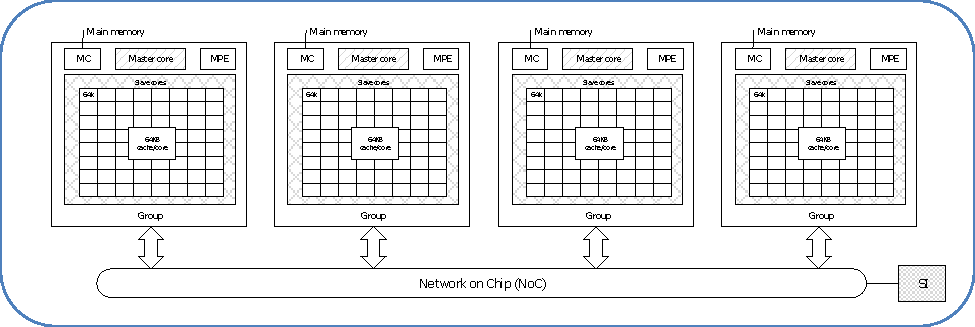
\includegraphics[scale=1]{\locpath/figures/Chap1/report_sunway_CPE}
\caption{Sunway Taihulight node architecture from \textit{Report on the Sunway TaihuLight System}, Jack Dongarra, June 24, 2016.}
\label{fig:chap1_report_sunway_CPE}
\end{figure}

The SW26010, a many core architecture processor, features 260 cores based on RISC architecture and a specific conception, depicted on figure~\ref{fig:chap1_report_sunway_CPE}. 
The processor is composed of the master core, a Memory Controller (MC) and a Management Processing Element (MPE) that manages the Computing Processing Elements (CPE), which are the slaves’ cores. 

The interconnect network is called Sunway Network and is connected using Mellanox Host Channel Adapter (HCA) and switches. 
This is a five-level interconnect going through computing nodes, computing board, super-nodes and cabinets to the complete system.
For the latest TOP500 list, from November 2017, the total memory is 1.31 PB and the number of cores available is 10,649,600.
The peak performance is 125.4 PFLOPS but the Linpack is only 93 PFLOPS which is 74.16\% of theoretic efficiency. 

\subsubsection{Piz Daint}
\index{Piz Daint}
The supercomputer of the CSCS, Swiss National Supercomputing Center, is currently ranked second on the November 2017 TOP500 list. 
This GPUs accelerated supercomputer is a most powerful representative of GPU hybrid acceleration and is the most powerful European supercomputer. 
This supercomputer is composed of 4761 hybrids and 1210 multi-core nodes. 
\index{NVIDIA}
There are hybrids nodes embedding an Intel Xeon E5-2690v3 and an NVIDIA Tesla Pascal P100 GPGPU. 
The interconnect is based on a Dragonfly network topology and Cray Aries routing and communications ASICs. 
The peak performance is 25.326 TFLOPS using only the hybrid nodes with Linpack generating 19.590 TFLOPS.
The low power consumption ranks Piz Daint as tenth in the November 2017 GREEN500.

\subsubsection{K-Computer}
\index{K-Computer}
The K-Computer was the top 1 supercomputer of the 2011 TOP500. 
The TOFU interconnect network makes the K-Computer unique~\cite{ajima2009tofu} and stands for TOrus FUsion.
\begin{figure}[t!]
\begin{center}
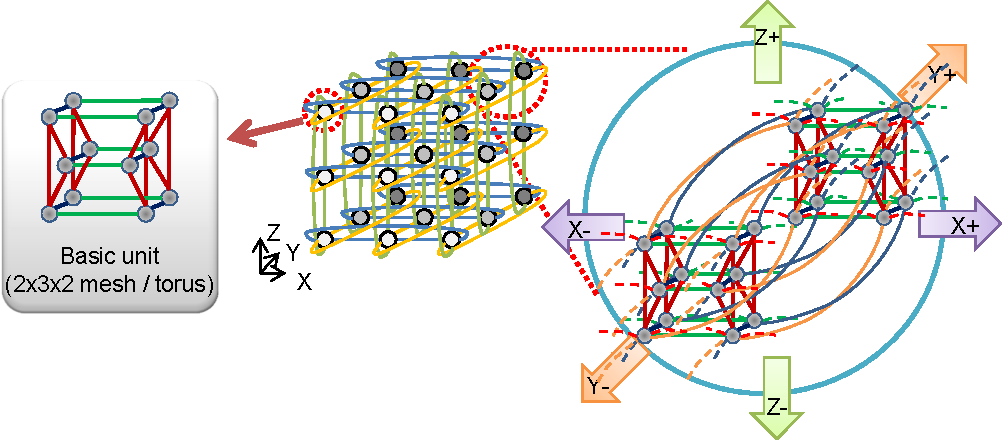
\includegraphics[width=\textwidth]{\locpath/figures/chap1/6d_torus}
\end{center}
\caption{TOFU Interconnect schematic from \textit{The K-Computer: System Overview}, Atsuya Uno, SC11}
\label{fig:1_HPC:tofu}
\end{figure}
\index{Interconnection}
This interconnect presented in figure~\ref{fig:1_HPC:tofu} mixes a 6D Mesh/Torus interconnect.
The basic units are based on a mesh and are interconnected together in a three-dimensional torus. 
In this configuration, each node can access to its 12 neighbors directly. 
It also provide a fault tolerant network with many routes to reach distant node. 

%\todo{AJouter MIRA/SEQUOIA pour paler de IBM, pour le Graph500 = meilleurs supercomputers}
%\todo{Parler de CRAY ?}
\subsubsection{Sequoia/Mira}
\index{IBM BlueGene}
The Sequoia supercomputer was ranked first on the 2012 TOP500 list. 
It is based on BlueGene from IBM.
The BlueGene project made up to three main architectures with BlueGene/L, BlueGene/P and BlueGene/Q.
It is very interesting to note the BlueGene architecture because 15 machine utilizing this architecture were in the top 200 in the last GRAPH500 list in November 2017.
The algorithm used on these supercomputers will be our basis in the Part II regarding our implementation of the GRAPH500 benchmark.

\section{ROMEO Supercomputer}
\index{ROMEO Supercomputer}
The ROMEO supercomputer center is the computation center of the Champagne-Ardenne region in France. 
Hosted since 2002 by the University of Reims Champagne-Ardenne, this so called meso-center (Medium size HPC center) is used for HPC in theoretic research and domain science like applied mathematics, physics, biophysics and chemistry. 

This project is supported by Europe, National Fundings, Grand-Est region and Reims Metropole. 
It aims to host research and production codes of the region for industrial, research and academics purposes. 

We are currently working on the fourth version of ROMEO, last updated in 2013. 
As many of our tests in this study have been done on this machine, we will carefully describe its architecture. 

This supercomputer was ranked 151st in the TOP500 and fifth in the GREEN500 list. 

\subsection{ROMEO hardware architecture}
\label{sec:part1_ROMEO}
ROMEO is a Bull/Atos supercomputer composed of 130 BullX R421 computing nodes. 

\index{K20Xm}
Each node is composed of two processors Intel Ivy Bridge 8 cores @ 2,6 GHz. 
Each processor has access to 16 GB of memory for a total of 32 GB per node, the total memory of 4.160 TB. 
Each processor is linked, using PCIe-v3, to an NVIDIA Tesla K20Xm GPGPU. 
This cluster provides then 260 processors for a total of 2080 CPU cores and 260 GPGPU providing 698880 GPU cores. 
The computation nodes are interconnected with an Infiniband QDR non-blocking network structured as a FatTree. 
The Infiniband is a QDR providing 10 GB/s. 

The storage for users is 57 TB and the cluster also provide 195 GB of Lustre and 88TB of parallel scratch file-system. 

In addition to the 130 computations nodes, the cluster provides a visualization node NVIDIA GRID with two K2 cards and 250GB of DDR3 RAM. 
The old machine, renamed Clovis, is also available but does not features GPUs. 

The supercomputer supports MPI with GPU Aware and GPUDirect. 

ROMEO is based on the Slurm\footnote{\url{https://slurm.schedmd.com/}} workload manager for node distribution among the users. 
This manager allows different usage of the cluster with classical reservation-submission or more asynchronous computation with best-effort. 
We developed advantages of both submissions systems in Part II. 

\subsection{New ROMEO supercomputer, June 2018}

In June 2018 a new version of the supercomputer ROMEO will be installed at the University of Reims Champagne Ardenne. 
This project intents to feature a supercomputer ranked around 250th in TOP500. 
It is a renewed partnership between ATOS/BULL and NVIDIA. 

The new ROMEO will feature 115 computation nodes with a total of 3220 CPU cores. 
The technology selected is the BULL \textit{Sequana} with its high energy saving, BXI network technology, NVLink support for GPUs and the density of the cluster. 
Each node will provide a Skylake 6132 CPU with 14 cores with a maximum frequency of 2.6GHz.

Two different types of node are present: 
\begin{itemize}[noitemsep,nolistsep]
\item[-] 70 of the with 4 GPUs and 96GB of RAM featuring a total of 280 Pascal P100 SMX2 GPUs.
\item[-] 45 last generation Intel CPUs with 192GB of memory per CPU. 
\end{itemize}

The machine will feature up to 15.3TB of global memory. 

The aim is to provide a performance of 964.6 TFLOPS in LINPACK and to be present in several TOP500 lists with a starting position around 232th or 297th. 

\section{Conclusion}

In this chapter, we reviewed the most important modern day hardware architectures and technologies. 
In order to use the driver or API in the most efficient way, we need to keep in mind the way the data and instructions are proceed by the machine. 

Efficiency is based on computation power, but also communications, we showed different interconnection topologies and their specificities. 
We present perfect use cases of the technologies in the current top ranked systems.
We show that every architecture is unique in its construction and justify the optimization work dedicated to reach performance. 

We determine from the new technologies presented here that supercomputers are moving toward hybrids architectures featuring multi-core processors accelerated by one or more devices such as many-core architectures. 
The Exascale supercomputer of 2020 will be shaped using hybrid architectures and they represent the best of nowadays technology for purpose of HPC this day and age. 
Combining CPU and GPUs or FPGA on the same die and sharing the same memory space may also be another solution.


%%%%%%%%%%%%%%%%%%%%%%%%%%%%%%%%%%%%%%%%%%%%%%%%%%%%%%%%%%%%%%%%%%%%%
%																	%
%	CHAPTER THREE, SOFTWARE AND API									%
%																	%
%%%%%%%%%%%%%%%%%%%%%%%%%%%%%%%%%%%%%%%%%%%%%%%%%%%%%%%%%%%%%%%%%%%%%

%%%%%%%%%%%%%%%%%%%%%%%%%%%%%%%%%%%%%%%%%%%%%%%%%%%%%%%%%%%%%%%%%%%%%
%								    %
%	CHAPTER THREE, SOFTWARE AND API				    %
%								    %
%%%%%%%%%%%%%%%%%%%%%%%%%%%%%%%%%%%%%%%%%%%%%%%%%%%%%%%%%%%%%%%%%%%%%


\chapter{Software and Benchmarks}

\section{Introduction}
After presenting the rules of HPC and the hardware that compose the cluster we need to introduice ways to target this supercomputer. 
Several options are present in the language, the multi-processing API, the distribution and the accelerators code. 
This chapter details the most important software options for HPC programming and include the choices we made for our applications.

Then it presents the software used to benchmark the supercomputers called Benchmarks. 
We present here the most famous, the TOP500, GRAPH500 and GREEN500 to give their advantages and weaknesses. 

\todo{Parler des pitfalls, load balancing, concurrence, ... ou le faire plus bas.}

\section{Sofware/API}
In this section we present the main runtimes, API and programming language use in HPC and in this study in particular. 
The considered language will be C/C++, the most present in HPC world.

\subsection{Parallel programming}
\subsubsection{PThreads}
The POSIX threads API is an execution model available in most of the languages. 
It allows the user to define threads that will execute concurrently on the processor ressources using shared/private memory.
PThreads is the low level handling of threads and the user need to handle concurrency with mutex, conditions variables and synchronization "by hand".
This makes the PThreads hard to use in complex applications and used only for very fine-grained control over the threads management. 
\todo{Fine-grain Coarse-grain applications}

\subsubsection{OpenMP}
Open Multi-Processing, OpenMP, is an API for multi-processing shared memory. 
It is based on the fork-join model.
\cite{chapman2008using,supinski2017scaling}

\subsubsection{Ohters}
Many other tools handle parallel programming for processors.
Cilk for C/C++ base, like OpenMP, on Fork-Join paradm. 
Threads Building Blocks, TBB, from Intel.

\subsection{Distributed}
In the cluster once the code have been developped locally and using the multiple cores available, the new step is to distribute it all over the nodes of the cluster. 
This step requires the processes to access NoRMA memory from a node to another. 
Several runtime are possible for this purpose.

\subsubsection{MPI}
The Message Passing Interface, MPI, is the most and widely spread runtime for distributed computing.
\cite{gropp2014using,gropp2015using}

\subsubsection{Charm++}
Charm++ is another API for distributed programming developped by the University of Illinois Urbana-Champaign.
It is based on asynchronous communications and futures/event mecanism. 

\subsubsection{Legion}

\subsection{Accelerators}
\subsubsection{CUDA}
The Compute Device Unified Architecture is the API developpe in C/C++ by NVIDIA to target its GPGPUs. 
\subsubsection{OpenCL}


\section{Benchmark}

\subsection{TOP500}
The most famous benchmark is certainly the TOP500\footnote{http://www.top500.org}. 
It gives the ranking of the 500 most powerful, known, supercomputers of the world as its name indicates.
Since 1993 the organization assembles and maintains this list updated twice a year in June and November.

This benchmark is based on the LINPACK\cite{dongarra1994top500} a benchmark introduced by Jack J. Dongarra.
This benchmark rely on solving  dense system of linear equations. 
As specified in this document this benchmark is just one of the tools to define the performance of a supercomputer. 
It reflects "the performance of a dedicated system for solving a dense system of linear equations".
This kind of benchmark is very regular in computation giving high results. 

\subsection{GRAPH500}
the GRAPH500 benchmark focus on irregular memory accesses, 


\subsection{GRENN500}

\section{Conclusion}




\chapter*{Conclusion}

% Chapter Two 
\part{Complex systems}
\chapter*{Introduction}

%%%%%%%%%%%%%%%%%%%%%%%%%%%%%%%%%%%%%%%%%%%%%%%%%%%%%%%%%%%%%%%%%%%%%
%                                                                   %
% CHAPTER ONE, Walls and pitfalls                                   % 
%                                                                   %
%%%%%%%%%%%%%%%%%%%%%%%%%%%%%%%%%%%%%%%%%%%%%%%%%%%%%%%%%%%%%%%%%%%%%

%%%%%%%%%%%%%%%%%%%%%%%%%%%%%%%%%%%%%%%%%%%%%%%%%%%%%%%%%%%%%%%%%%%%%
%                                                                   %
%	CHAPTER ONE, CHOICES AND SPH                                    %
%                                                                   %
%%%%%%%%%%%%%%%%%%%%%%%%%%%%%%%%%%%%%%%%%%%%%%%%%%%%%%%%%%%%%%%%%%%%%
\chapter{General problem}

\section{Introduction}
In this section we give details on our choices for the generic application confronted to both computation and communication walls in irregular context. 
This problem, the Smoothed Particle Hydrodynamics method implementation, is described on the physics aspect and the difficulties involved in the resolution on supercomputers and accelerators.  

\section{Smoothed Particle Hydrodynamics}

\subsection{General description}
Smoothed Particle Hydrodynamics (SPH) is an explicit numerical mesh-free Lagrangian method.
It is used to solve hydrodynamical partial differential equations (PDEs) by discretized them into a set of fluid elements called particles. 
This computational method was invented for the purpose of astrophysics simulations by Monaghan, Gingold and Lucy in 1977 \cite{lucy1977numerical,gingold1977smoothed}. 
This first SPH work conserved mass and they later proposed a method which also conserves linear and angular moment \cite{gingold1982kernel}. 
The method was extended for general fluid simulation and many more fields from ballistics to oceanography.
The development of new reliable, parallel and distributed tools for this method is a challenge for future HPC architectures with the upcoming Exascale systems.

\begin{figure}
\centering
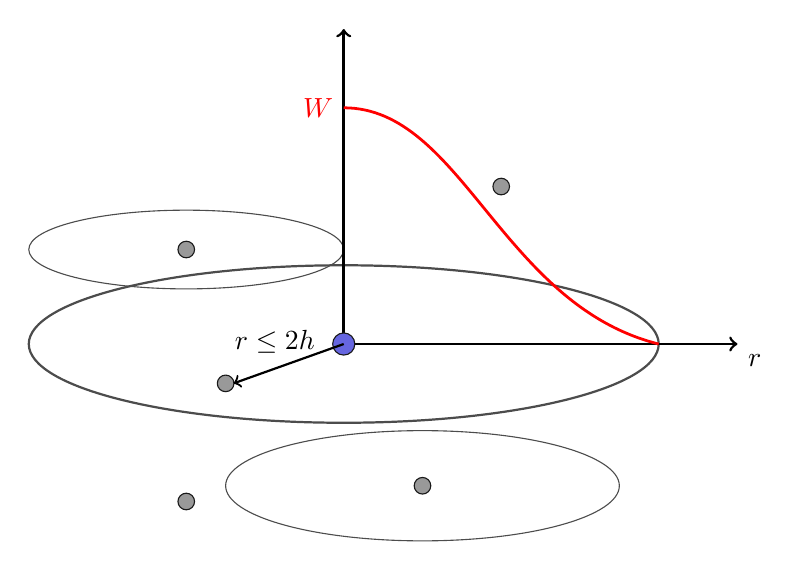
\begin{tikzpicture}
	
	% Others and their ellipse
	\draw [black!90,fill=black!40] (.5,1.5) circle (.3em);
	\draw [black!90,fill=black!40] (0,0) circle (.3em);
	\draw [black!90,fill=black!40] (0,3.2) circle (.3em);
	\draw[black!70] (0,3.2) ellipse (2 and .5);
	\draw [black!90,fill=black!40] (3,.2) circle (.3em);
	\draw[black!70] (3,.2) ellipse (2.5 and .7);
	\draw [black!90,fill=black!40] (4,4) circle (.3em);
	% Ellipses 
	\draw[line width=.8pt,black!70] (2,2) ellipse (4 and 1);
	% Axes
	\draw[->,line width=1pt] (2,2) -- (7,2) node[anchor=north west] {$r$};
	\draw[->,line width=1pt] (2,2) -- (2,6);
	% bezier for kernel 
	\draw[red,line width=1pt]  (6,2) .. controls (4,2.5) and (3.5,5) .. (2,5) node[red,anchor=east] {$W$};
	% main particle, at the end to cover
	\draw [black!90,fill=black!20!blue!60] (2,2) circle (.4em);
	% Arrows 
	\draw[->,line width=.8pt] (2,2) -- (.6,1.5) node[midway, above,xshift=-.5em] {$r\leq2h$};
\end{tikzpicture}
%\includegraphics[scale=.4]{\locpath/figures/flecsph/sph.pdf}
\caption{SPH kernel $W$ and smoothing length $h$ representation}
\label{fig:sph_base}
\end{figure}

The method, as illustrated in figure~\ref{fig:sph_base}, computes the evolution of physical quantities for every particle regarding its neighbors in the radius of its smoothing length $h$. 
The particles in this radius are then valued according to their distance using a smoothing function $W$, also called a kernel. 
The fundamental SPH formulation for any physical quantity $A$ is then to compute with all the neighbors of $b$ of a particle by:
\begin{equation}
A(\vec{r}) \simeq \sum_b \frac{m_b}{\rho_b} A(\vec{r}_b) W ( |\vec{r}-\vec{r}_b|,h)
\end{equation}

On a physics aspect, this method has several advantages:
It can handle deformations, low densities, vacuum, and makes particle tracking easier. 
It also conserves mass, linear and angular momenta, and energy by its construction that implies independence of the numerical resolution. 
Another strong benefit of using SPH is its exact advection of fluid properties. 
Furthermore, the particle structure of SPH easily combines with tree methods for solving Newtonian gravity through N-body simulations.
As a mesh-free method, it avoids the need of grid to calculate the spatial derivatives. 

However, there are cons to consider using SPH: 
It is restricted to low-order rate of convergence on certain PDE formulations; 
It requires careful setup of initial distribution of particles; 
Further, it can be struggle to resolve turbulence-dominated flows and special care must be taken when handling high gradients such as shocks and surface structure of neutron stars.
Many works are leading to handle more cases and to push the limitations of this method \cite{dai2017dual,lind2016incompressible,ren2016dual}.

In this work, we are solving Lagrangian conservation equations (Euler equations) for mass, energy and momentum of an ideal fluid ~\cite{Landau1959}  such that:
\begin{equation}
\frac{d \rho}{d t} = - \rho \nabla \cdot \vec{v}, \quad
\frac{d u}{d t} = \left( \frac{P}{\rho^2} \right) \frac{d \rho}{d t}, \quad
\frac{d \vec{v}}{d t} = - \frac{\nabla P}{\rho}
\end{equation}
with $\rho$ the density, $P$ the pressure, $u$ the internal energy and $v$ the velocity, where $d/dt = \partial_t + \vec{v} \cdot \nabla$ which is convective derivative.

By using the volume element $V_b = m_b / \rho_b$, we can formulate the Newtonian SPH scheme~\cite{rosswog2009} such that
\begin{equation}
\label{eq:rho}
\rho_a = \sum_b m_b W_{ab} (h_a)
\end{equation}
\begin{equation}
\frac{d u_a}{dt} = \frac{P_a}{\rho_a^2} \sum_b m_b \vec{v}_{ab} \cdot \nabla_a W_{ab} 
\end{equation}
\begin{equation}
\frac{d \vec{v}_a}{d t} = - \sum_b m_b \left(\frac{P_a}{\rho_a^2} + \frac{P_b}{\rho_b^2} \right) \nabla_a W_{ab}
\end{equation}
where $W_{ab} = W(| \vec{r}_a - \vec{r}_b |,h)$ is the smoothing kernel. 
The equations we would like to solve allow for emergence of discontinuities from smooth initial data. 
At discontinuities, the entropy increases in shocks. That dissipation occurs inside the shock-front. 
The SPH formulation here is inviscid so we need to handle this dissipation near shocks. 
There are a number of way to handle this problem, but the most widespread approach is to add artificial viscosity (or artificial dissipation) terms in SPH formulation such that:
\begin{equation}
\left(\frac{d u_a}{dt} \right)_{art} = \frac{1}{2} \sum_b m_b \Pi_{ab} \vec{v}_{ab} \cdot \nabla_a W_{ab}
\end{equation}
\begin{equation}
\left(\frac{d\vec{v}_a}{dt} \right)_{art} = - \sum_b m_b \Pi_{ab}\nabla_a W_{ab}
\end{equation}
In general, we can express the equations for internal energy and acceleration with artificial viscosity
\begin{equation}
\label{eq:intern}
\frac{d u_a}{dt} = \sum_b m_b \left(\frac{P_a}{\rho_a^2} + \frac{\Pi_{ab}}{2} \right) \vec{v}_{ab} \cdot \nabla_a W_{ab}
\end{equation}
\begin{equation}
\label{eq:velo}
\frac{d \vec{v}_a}{d t} = - \sum_b m_b \left(\frac{P_a}{\rho_a^2} + \frac{P_b}{\rho_b^2} + \Pi_{ab} \right) \nabla_a W_{ab}
\end{equation}
$\Pi_{ab}$ is the artificial viscosity tensor. 
As long as $\Pi_{ab}$ is symmetric, the conservation of energy, linear and angular momentum is assured by the form of the equation and antisymmetry of the gradient of kernel with respect to the exchange of indices $a$ and $b$. $\Pi_{ab}$ may define different way but here we use~\cite{Monaghan1983} such as: 
\begin{equation}
\Pi_{ab} = \begin{cases}
\frac{- \alpha \bar{c}_{ab} \mu_{ab} + \beta \mu_{ab}^2}{\bar{\rho}_{ab}} & \text{for $\vec{r}_{ab} \cdot \vec{v}_{ab} < 0$} \\
0 & \text{otherwise}
\end{cases}
\end{equation}
\begin{equation}
\mu_{ab} = \frac{\bar{h}_{ab} \vec{r}_{ab} \cdot \vec{v}_{ab}}{r^2_{ab} + \epsilon \bar{h}_{ab}^2}
\end{equation}

Using the usual form $c_s$ as $c_s = \sqrt{\frac{\partial p}{\partial \rho}}$.
The values of $\epsilon$, $\alpha$, and $\beta$ have to be set regarding the problem targeted. 
Here, we use $\epsilon = 0.01h^2$, $\alpha = 1.0$, and $\beta = 2.0$. 

There are many possibilities for the smoothing function, called the kernel. 
As an example the Monaghan's cubic spline kernel is given by:
\begin{equation}
W(\vec{r},h) = \frac{\sigma}{h^D} \begin{cases}
1-\frac{3}{2} q^2 + \frac{3}{4} & \text{if} \indent 0 \leq q \leq 1 \\
\frac{1}{4} (1-q)^3  & \text{if} \indent 1 \leq q \leq 2 \\
0 & \text{otherwise}
\end{cases}
\end{equation}
where $q = r/h$, $r$ the distance between the two particles, $D$ is the number of dimensions and $\sigma$ is a normalization constant with the values:
\begin{equation}
\sigma =  \begin{cases}
\frac{2}{3} & \text{for 1D}  \\
\frac{10}{7 \pi} & \text{for 2D} \\
\frac{1}{\pi} & \text{for 3D}
\end{cases}
\end{equation}

To sum up, the SPH resolution scheme and its routines are presented on algorithm \ref{alg:sph}.
The Equation of State (EOS) and the integration are problem dependent and will be define for each test case in section \ref{sec:applications}. 

\begin{algorithm}
\caption{SPH loop algorithm}\label{alg:sph}
\begin{algorithmic}[1]
\While{not last step}
\State Compute density for each particle (\ref{eq:rho})
\State Compute pressure using EOS 
\State Compute acceleration from pressure forces (\ref{eq:velo})
\State Compute change of internal energy for acceleration (\ref{eq:intern})
\State Advance particles after integration
\EndWhile
\end{algorithmic}
\end{algorithm}

The main downside for the implementation of this method is the requirement for local computation on every particle. 
The particles have to be grouped locally to perform the computation of (\ref{eq:rho}), (\ref{eq:intern}) and (\ref{eq:velo}).
A communication step is needed before and after (\ref{eq:rho}) to get the local physical data to be able to compute (\ref{eq:intern}) and (\ref{eq:velo}).
The tree data structure allows us to perform $O(Nlog(N))$ neighbor search but also add a domain decomposition and distribution layer.

As the SPH method is used in a large panel of fields from astrophysics to fluid mechanic, there are numerous related works. 
We can cite a code developed in the LANL, 2HOT \cite{warren20132hot} that introduced the Hashed Oct Tree structure used in our implementation. 
There is also GADGET-2 \cite{springel2005cosmological}, GIZMO \cite{hopkins2014gizmo} and the most recent publication is GASOLINE \cite{wadsley2017gasoline2} based on PKDGRAV, a specific tree+gravity implementation. 
Several implementations already implement GPU code and tree construction and traversal, one can cite GOTHIC \cite{miki2017gothic}, presenting gravitational tree code accelerated using the latest Fermi, Kepler and Maxwell architectures. But a lot of GPU accelerated work still focused on fluid problems and not on astrophysical problems  \cite{harada2007smoothed,crespo2011gpus}.
We also note that these implementations focus on SPH problems and does not provide a general purpose and multi-physics framework like we intent to provide through FleCSPH and FleCSI. 

\subsection{Gravitation}
For classical problems like fluid flow the gravitation can directly be applied on the particles with the force:
\begin{equation}
	\vec{a_g} = m\vec{g}
\end{equation}

In order to consider astrophysics problems we need to introduice self-gravitation. 
Each particle imply an action on the others base on its distance and mass. 
The equation of gravitation for a particle $i$ with $j$ other particles is: 
\begin{equation}
	\vec{f_a}_i = \sum_j -G \frac{m_i m_j}{|\vec{r_i}-\vec{r_j}|^3} \vec{r_{ij}}
	\label{eq:gravitation}
\end{equation}

This computation involve an $O(N^2)$ complexity and thus is not applicable directly. 
We applied the method called Fast Multipole Method, FMM and discussed in \cite{beatson1997short}.
In this method we compute the gravitation up a approximations. 
The user can refine those approximation changing parameters. 

\begin{figure}
\resizebox {\columnwidth} {!} {
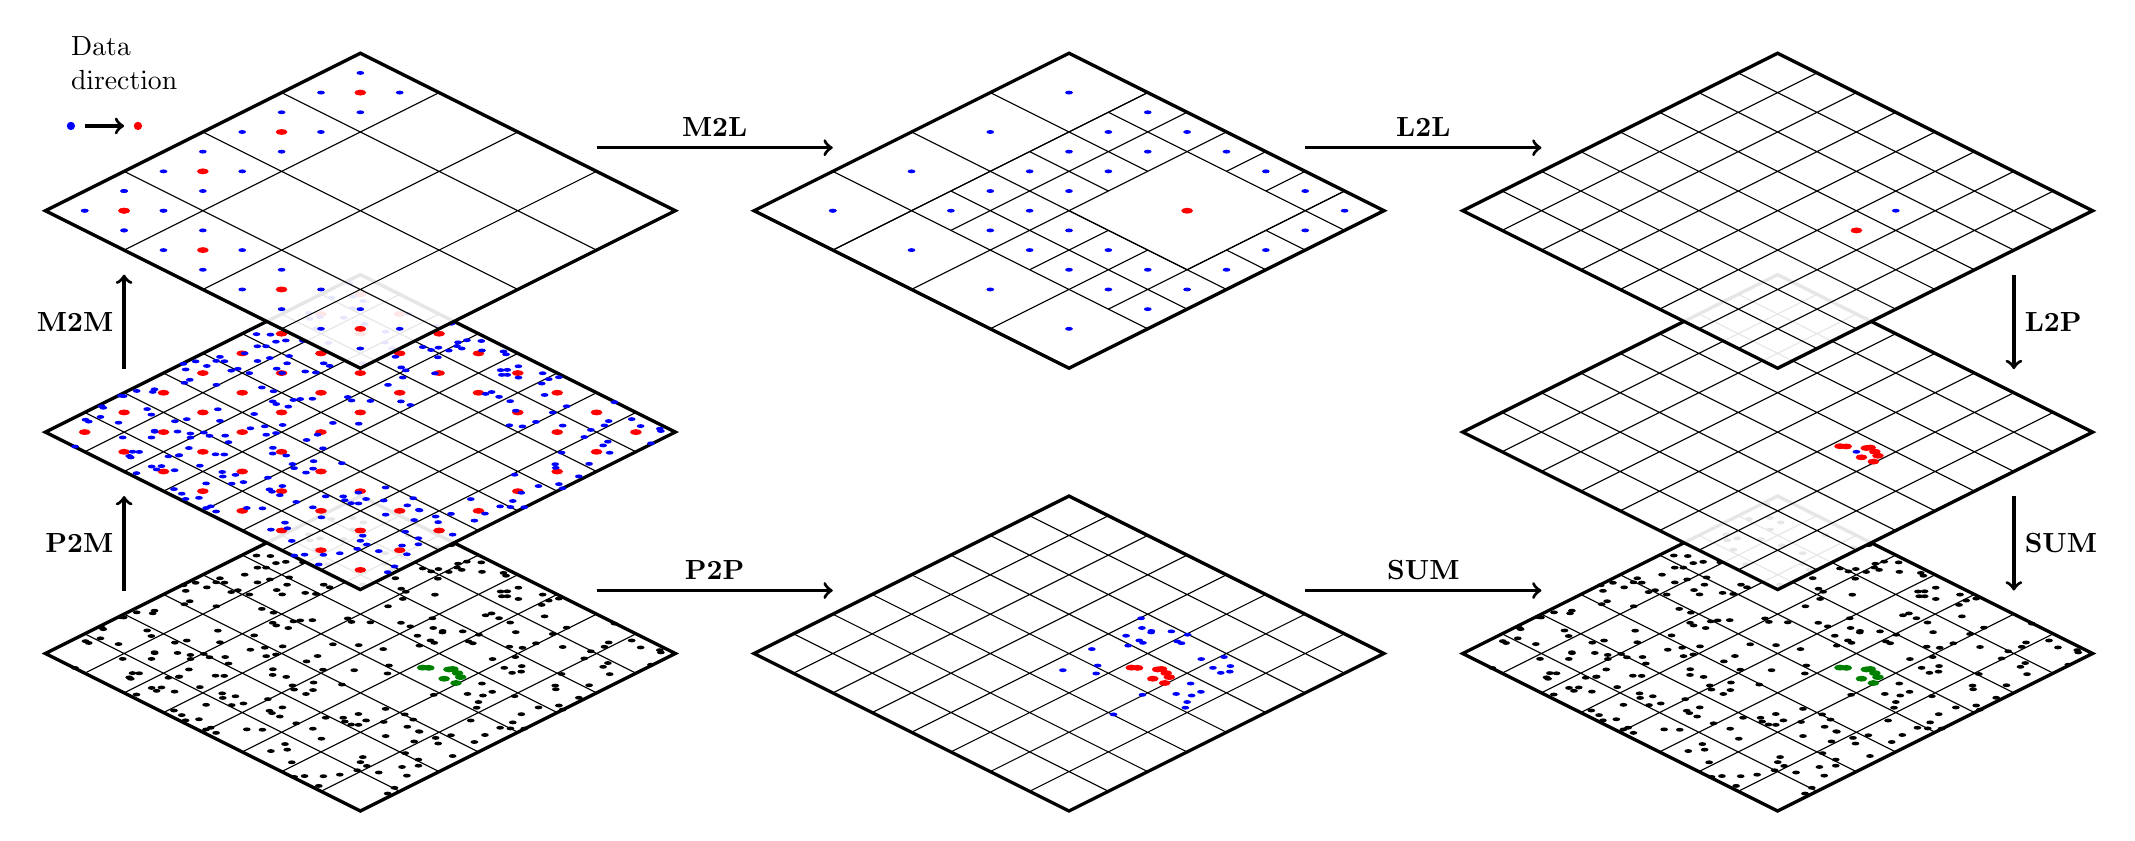
\begin{tikzpicture}
\def\nrand{300}
\def\seed{12}
\def\gridSize{5mm}
\def\gridTotal{4}
% Particles to Multipole
\pgfmathsetseed{\seed}
\begin{scope}[
   		yshift=0,every node/.append style={
    		yslant=0.5,xslant=-1},yslant=0.5,xslant=-1
    ]
    \fill[white,fill opacity=.9] (0,0) rectangle (4,4);
    \draw[black,very thick] (0,0) rectangle (4,4);
	\draw[step=\gridSize, black] (0,0) grid (\gridTotal,\gridTotal);
	\foreach \i in {1,2,...,\nrand}{
    	\pgfmathsetmacro{\x}{(rand)*2+2}
    	\pgfmathsetmacro{\y}{(rand)*2+2}
		% COLOR 
		\ifthenelse{\( \lengthtest{\x cm>2cm} \AND \lengthtest{\x cm<2.5cm} \)}
		{	
			\ifthenelse{ \( \lengthtest{\y cm>1cm} \AND \lengthtest{\y cm<1.5cm} \)}
			{\node at (\x,\y) [black!50!green,circle,fill,inner sep=.7pt,minimum size=3pt]{};}
			{\node at (\x,\y) [circle,fill,inner sep=.7pt]{};}
		}
		{\node at (\x,\y) [circle,fill,inner sep=.7pt]{};}
	}
\end{scope}
\pgfmathsetseed{\seed}
\begin{scope}[
   		yshift=80,every node/.append style={
    		yslant=0.5,xslant=-1},yslant=0.5,xslant=-1
    ]
    \fill[white,fill opacity=.9] (0,0) rectangle (4,4);
    \draw[black,very thick] (0,0) rectangle (4,4);
	\draw[step=5mm, black] (0,0) grid (\gridTotal,\gridTotal);
	\foreach \x in {0,1,...,7}{\foreach \y in {0,1,...,7}{
		\ifthenelse{\( \x<3 \OR \x>5 \)}
		{
			\node at (\x*\gridSize+\gridSize/2,\y*\gridSize+\gridSize/2)[red,circle,fill,inner sep=.7pt,minimum size=3pt]{};
		}
		{	\ifthenelse{ \( \y<1 \OR \y>3 \)}
			{
			\node at (\x*\gridSize+\gridSize/2,\y*\gridSize+\gridSize/2)[red,circle,fill,inner sep=.7pt,minimum size=3pt]{};	
			}{}
		}
	}}
	\foreach \i in {1,2,...,\nrand}{
    	\pgfmathsetmacro{\x}{(rand)*2+2}
    	\pgfmathsetmacro{\y}{(rand)*2+2}
    	\ifthenelse{\( \lengthtest{\x cm<1.5cm} \OR \lengthtest{\x cm>3cm} \)}
		{\node at (\x,\y) [blue,circle,fill,inner sep=.7pt]{};}
		{	\ifthenelse{ \( \lengthtest{\y cm<.5cm} \OR \lengthtest{\y cm>2cm} \)}
			{\node at (\x,\y) [blue,circle,fill,inner sep=.7pt]{};}
			{}
		}
  	}
\end{scope}
\begin{scope}[
   		yshift=160,every node/.append style={
    		yslant=0.5,xslant=-1},yslant=0.5,xslant=-1
    ]
    \fill[white,fill opacity=.9] (0,0) rectangle (4,4);
    \draw[black,very thick] (0,0) rectangle (4,4);
	\draw[step=10mm, black] (0,0) grid (4,4);
	\foreach \x in {0,1}{\foreach \y in {0,...,7}{
		\node at (\x*\gridSize+\gridSize/2,\y*\gridSize+\gridSize/2)[blue,circle,fill,inner sep=.7pt]{};
	}}
	\foreach \x in {0,...,7}{\foreach \y in {6,7}{
		\node at (\x*\gridSize+\gridSize/2,\y*\gridSize+\gridSize/2)[blue,circle,fill,inner sep=.7pt]{};
	}}

	\foreach \x in {0}{\foreach \y in {0,...,3}{				  
		\node at (\x*\gridSize*2+\gridSize,\y*\gridSize*2+\gridSize) [red,circle,fill,inner sep=.7pt,minimum size=3pt]{};
	}}
	\foreach \x in {0,...,3}{\foreach \y in {3}{				  
		\node at (\x*\gridSize*2+\gridSize,\y*\gridSize*2+\gridSize) [red,circle,fill,inner sep=.7pt,minimum size=3pt]{};
	}}
\end{scope}

%PARTICLES TO PARTICLES
\pgfmathsetseed{\seed}
\begin{scope}[
   		yshift=0,xshift=9cm,every node/.append style={
    		yslant=0.5,xslant=-1},yslant=0.5,xslant=-1
    ]
    \fill[white,fill opacity=.9] (0,0) rectangle (4,4);
    \draw[black,very thick] (0,0) rectangle (4,4);
	\draw[step=5mm, black] (0,0) grid (4,4);
	\foreach \i in {1,2,...,\nrand}{
    	\pgfmathsetmacro{\x}{(rand)*2+2}
    	\pgfmathsetmacro{\y}{(rand)*2+2}
    	\ifthenelse{\( \lengthtest{\x cm>1.5cm} \AND \lengthtest{\x cm<3cm} \)}
		{	
			\ifthenelse{ \( \lengthtest{\y cm>.5cm} \AND \lengthtest{\y cm<2cm} \)}
			{
				% COLOR 
				\ifthenelse{\( \lengthtest{\x cm>2cm} \AND \lengthtest{\x cm<2.5cm} \)}
				{	
					\ifthenelse{ \( \lengthtest{\y cm>1cm} \AND \lengthtest{\y cm<1.5cm} \)}
					{\node at (\x,\y) [red,circle,fill,inner sep=.7pt,minimum size=3pt]{};}
					{\node at (\x,\y) [blue,circle,fill,inner sep=.7pt]{};}
				}
				{\node at (\x,\y) [blue,circle,fill,inner sep=.7pt]{};}
			}{}
		}{}
    	%\node at (\x,\y) [circle,fill,inner sep=.7pt]{};
  	}
\end{scope}
%MULTIPOLE TO MULTIPOLE
\begin{scope}[
   		yshift=160,xshift=9cm,every node/.append style={
    		yslant=0.5,xslant=-1},yslant=0.5,xslant=-1
    ]
    \fill[white,fill opacity=.9] (0,0) rectangle (4,4);
    \draw[black,very thick] (0,0) rectangle (4,4);
    \draw[step=10mm, black] (0,3) grid (4,4);
	\draw[step=10mm, black] (0,0) grid (1,3);
	\draw[step=5mm, black] (1,0) grid (2,3);
	\draw[step=5mm, black] (2,2) grid (4,3);
	\draw[step=5mm, black] (2,0) grid (4,.5);
	\draw[step=5mm, black] (3.5,0) grid (4,2);
	% add rectangle
	\draw[black] (2,.5) rectangle (3.5,2);
	% Big part 
	\foreach \x in {0}{\foreach \y in {0,...,3}{				  
		\node at (\x*\gridSize*2+\gridSize,\y*\gridSize*2+\gridSize) [blue,circle,fill,inner sep=.7pt]{};
	}}
	\foreach \x in {0,...,3}{\foreach \y in {3}{				  
		\node at (\x*\gridSize*2+\gridSize,\y*\gridSize*2+\gridSize) [blue,circle,fill,inner sep=.7pt]{};
	}}
	% Smaller one 
	\foreach \x in {2,3}{\foreach \y in {0,...,3}{
		\node at (\x*\gridSize+\gridSize/2,\y*\gridSize+\gridSize/2)[blue,circle,fill,inner sep=.7pt]{};
	}}

	\foreach \x in {2,...,7}{\foreach \y in {4,5}{
		\node at (\x*\gridSize+\gridSize/2,\y*\gridSize+\gridSize/2)[blue,circle,fill,inner sep=.7pt]{};
	}}

	\foreach \x in {7}{\foreach \y in {0,...,3}{
		\node at (\x*\gridSize+\gridSize/2,\y*\gridSize+\gridSize/2)[blue,circle,fill,inner sep=.7pt]{};
	}}
	\foreach \x in {4,5,6}{\foreach \y in {0}{
		\node at (\x*\gridSize+\gridSize/2,\y*\gridSize+\gridSize/2)[blue,circle,fill,inner sep=.7pt]{};
	}}
	\node at (5*\gridSize+\gridSize/2,2*\gridSize+\gridSize/2) [red,circle,fill,inner sep=.7pt,minimum size=3pt]{};
\end{scope}

% Multipole to Particles 
\pgfmathsetseed{\seed}
\begin{scope}[
   		yshift=0,xshift=18cm,every node/.append style={
    		yslant=0.5,xslant=-1},yslant=0.5,xslant=-1
    ]
    \fill[white,fill opacity=.9] (0,0) rectangle (4,4);
    \draw[black,very thick] (0,0) rectangle (4,4);
	\draw[step=5mm, black] (0,0) grid (4,4);
	\foreach \i in {1,2,...,\nrand}{
    	\pgfmathsetmacro{\x}{(rand)*2+2}
    	\pgfmathsetmacro{\y}{(rand)*2+2}
		% COLOR 
		\ifthenelse{\( \lengthtest{\x cm>2cm} \AND \lengthtest{\x cm<2.5cm} \)}
		{	
			\ifthenelse{ \( \lengthtest{\y cm>1cm} \AND \lengthtest{\y cm<1.5cm} \)}
			{\node at (\x,\y) [black!50!green,circle,fill,inner sep=.7pt,minimum size=3pt]{};}
			{\node at (\x,\y) [circle,fill,inner sep=.7pt]{};}
		}
		{\node at (\x,\y) [circle,fill,inner sep=.7pt]{};}
	}
\end{scope}
\pgfmathsetseed{\seed}
\begin{scope}[
   		yshift=80,xshift=18cm,every node/.append style={
    		yslant=0.5,xslant=-1},yslant=0.5,xslant=-1
    ]
    \fill[white,fill opacity=.9] (0,0) rectangle (4,4);
    \draw[black,very thick] (0,0) rectangle (4,4);
	\draw[step=5mm, black] (0,0) grid (4,4);

	\foreach \i in {1,2,...,\nrand}{
    	\pgfmathsetmacro{\x}{(rand)*2+2}
    	\pgfmathsetmacro{\y}{(rand)*2+2}
    	\ifthenelse{\( \lengthtest{\x cm>1.5cm} \AND \lengthtest{\x cm<3cm} \)}
		{	
			\ifthenelse{ \( \lengthtest{\y cm>.5cm} \AND \lengthtest{\y cm<2cm} \)}
			{
				% COLOR 
				\ifthenelse{\( \lengthtest{\x cm>2cm} \AND \lengthtest{\x cm<2.5cm} \)}
				{	
					\ifthenelse{ \( \lengthtest{\y cm>1cm} \AND \lengthtest{\y cm<1.5cm} \)}
					{\node at (\x,\y) [red,circle,fill,inner sep=.7pt,minimum size=3pt]{};}
					{}
				}{}
			}{}
		}{}
	}
	\node at (4*\gridSize+\gridSize/2,2*\gridSize+\gridSize/2) [blue,circle,fill,inner sep=.7pt]{};
\end{scope}
%% MULTIPOLE TO LOCAL
\begin{scope}[
   		yshift=160,xshift=18cm,every node/.append style={
    		yslant=0.5,xslant=-1},yslant=0.5,xslant=-1
    ]
    \fill[white,fill opacity=.9] (0,0) rectangle (4,4);
    \draw[black,very thick] (0,0) rectangle (4,4);
	\draw[step=5mm, black] (0,0) grid (4,4);
	\node at (4*\gridSize+\gridSize/2,2*\gridSize+\gridSize/2) [red,circle,fill,inner sep=.7pt,minimum size=3pt]{};

	\node at (5*\gridSize+\gridSize/2,2*\gridSize+\gridSize/2) [blue,circle,fill,inner sep=.7pt]{};
\end{scope}
% ARROWS AND TEXT
\draw[->,very thick] (-3,2.8) -- (-3,4) node[midway,left] {\textbf{P2M}};
\draw[->,very thick] ([yshift=80]-3,2.8) -- ([yshift=80]-3,4) node[midway,left] {\textbf{M2M}};

\draw[->,very thick] ([yshift=160]3,2.8) -- ([yshift=160]6,2.8) node[midway,above] {\textbf{M2L}};
\draw[->,very thick] ([yshift=160,xshift=9cm]3,2.8) -- ([yshift=160,xshift=9cm]6,2.8) node[midway,above] {\textbf{L2L}};

\draw[<-,very thick] ([yshift=80]21,2.8) -- ([yshift=80]21,4) node[midway,right] {\textbf{L2P}};
\draw[<-,very thick] (21,2.8) -- (21,4) node[midway,right] {\textbf{SUM}};

\draw[->,very thick] (3,2.8) -- (6,2.8) node[midway,above] {\textbf{P2P}};
\draw[->,very thick] ([xshift=9cm]3,2.8) -- ([xshift=9cm]6,2.8) node[midway,above] {\textbf{SUM}};


\draw[->,very thick] (-3.5,8.7cm) node[xshift=-5pt,blue,circle,fill,inner sep=.7pt,minimum size=3pt] (a) {} -- 
 (-3,8.7cm) node[xshift=5pt,red,circle,fill,inner sep=.7pt,minimum size=3pt] (b) {};
\node[align=left] at (-3,9.5cm) {Data\\direction};


\end{tikzpicture}
}
\caption{Fast Multipole Method schematics. Particles to Multipole (P2M), Multipole to Multipole (M2M), Multipole to Particles (M2P), Multipole to Local (M2L), Local to Local (L2L) and Particles to Particles (P2P). Schematic inspired from \cite{yokota2011treecode}}
\end{figure}

This method is based on Taylor series.
The gravitation function of equation~\ref{eq:gravitation} can be approximate on a particle at position $\vec{r}$ by the gravitation computed at the centroid at position $\vec{r_c}$: 
\begin{equation}
 \vec{f}(\vec{r}) = \vec{f}(\vec{r_c}) + ||\frac{\partial\vec{f}}{\partial\vec{r}}||\cdot (\vec{r} - \vec{r_c}) + \frac{1}{2} (\vec{r}-\vec{r_c})^\intercal \cdot   ||\frac{\partial\vec{f}}{\partial\vec{r} \partial\vec{r}}|| \cdot (\vec{r} - \vec{r_c})
 \end{equation}

 From equation~\ref{eq:gravitation} we compute the term $||\frac{\partial\vec{f}}{\partial\vec{r}}||$:s
 \begin{equation}
\frac{\partial\vec{f}}{\partial\vec{r}} =
- \sum_p \frac{m_p}{|\vec{r_c}-\vec{r_p}|^3}
\begin{bmatrix}
1 - \frac{3(x_c-x_p)(x_c-x_p)}{|\overline{r_c}-\overline{r_p}|^2} & -\frac{3(y_c-y_p)(x_c-x_p)}{|\overline{r_c}-\overline{r_p}|^2}  & -\frac{3(z_c-z_p)(x_c-x_p)}{|\vec{r_c}-\vec{r_p}|^2}  \\
-\frac{3(x_c-x_p)(y_c-y_p)}{|\vec{r_c}-\vec{r_p}|^2}  & 1 - \frac{3(y_c-y_p)(y_c-y_p)}{|\vec{r_c}-\vec{r_p}|^2} &  -\frac{3(z_c-z_p)(y_c-y_p)}{|\vec{r_c}-\vec{r_p}|^2}\\
- \frac{3(x_c-x_p)(z_c-z_p)}{|\vec{r_c}-\vec{r_p}|^2}   &  -\frac{3(y_c-y_p)(z_c-z_p)}{|\vec{r_c}-\vec{r_p}|^2} &  1- \frac{3(z_c-z_p)(z_c-z_p)}{|\vec{r_c}-\vec{r_p}|^2} \\
\end{bmatrix}
 \end{equation}

And we propose a compact version of the matrix with: 
 
\begin{equation}
 ||\frac{\partial f^a}{\partial r^b}|| = -\sum_c \frac{m_c}{|\vec{r}-\vec{r_c}|^3} \Big[ \delta_{ab} - \frac{3.(r^a-r_c^a)(r^b-r_c^b)}{|\vec{r}-\vec{r_c}|^2} \Big] 
\end{equation}

With $\delta_{ab}$ the Kronecker delta:
\begin{equation}
\delta_{ab} = 
\begin{cases}
    1, & \text{if $a = b$}.\\
    0, & \text{if $a\neq b$}.
  \end{cases}
\end{equation}

We note that $a$ and $b$ variate from 0 to 2 and $r^0=x$, $r^1=y$, and $r^2=z$ as usual sense. 

For the term $||\frac{\partial\vec{f}}{\partial\vec{r} \partial\vec{r}}||$ we give the compact version by:
\begin{equation}
\begin{aligned}
||\frac{\partial^2 f^a}{\partial r^b \partial r^c}|| = - \sum_c \frac{3 m_c}{|\vec{r}-\vec{r_c}|^5} \Big[ & \frac{5(r^a-r_c^a)(r^b-r_c^b)(r^c-r_c^c)}{|\vec{r}-\vec{r_c}|^2} - \\ 
		 & \left( \delta_{ab} (r^c-r_c^c)+\delta_{bc} (r^a-r_c^a)+\delta_{ac} (r^b-r_c^b) \right) \Big] 
\end{aligned}
\end{equation} 

 \begin{figure}
 \end{figure}

The method is summed up in figure with the different equations.
We consider Centers Of Mass, COM, to be the centroid of particles based on their position. 
In several steps the information is first transmitted to the COMs, computing their position and mass. 


\section{Applications of SPH} 
The previous equations are generic and describe the behavior of SPH method. 
In order to check our 

\subsection{Sod shock tube}
The Sod shock tube is the test consisting of a one-dimensional Riemann problem with the following initial parameters~\cite{sod1978}.
\begin{equation}
(\rho, v, p)_{t=0} = \begin{cases}
(1.0,0.0,1.0) & \text{if} \indent 0 < x \leq 0.5 \\
(0.125,0.0,0.1) & \text{if} \indent 0.5 < x < 1.0
\end{cases}
\end{equation}
In our code, we use the same initial data as in section \ref{sec:intro_sph} with ideal gas EOS such as:
\begin{equation}
P(\rho,u) = (\Gamma - 1) \rho u
\end{equation}
where $\Gamma$ is the adiabatic index of the gas, we set $\Gamma = 5/3$. 

\begin{figure}[t!]
\centering
\includegraphics[width=\columnwidth]{\locpath/figures/sph/{sodtube_width}.png}
\caption{Sod shock tube with FleCSPH}
\label{fig:sodtube}
\end{figure}

This test is used to check the physical accuracy of the code and thus the tree search itself.
A simulation of our Sod shock experimentation is presented on Fig.~\ref{fig:sodtube} and shows physically correct results. 

\subsection{Sedov blast wave}
A blast wave is the pressure and flow resulting from the deposition of a large amount of energy in a small very localized volume. 
There are different versions of blast wave test and we consider comparing it with the analytic solution for a point explosion as given by Sedov~\cite{sedov1946}, making the assumption that the atmospheric pressure relative to the pressure insider the explosion negligible. 
Here, we test 2D blast wave. In this simulation, we use ideal gas EOS with $\Gamma = 5/3$ and we are assuming that the undistributed area is at rest with a pressure $P_0 = 1.0 \time 10^{-5}$. The density is constant $\rho_0$, also in the pressurized region. 

\begin{figure}[t]
\centering
\includegraphics[width=\columnwidth]{\locpath/figures/sph/{sedov_flecsph_results}}
\caption{Sedov Blast Wave with FleCSPH at respectively $t=0.01$, $t=0.03$, $t=0.06$ and $t=0.1$}
\label{fig:sedov}
\end{figure}

An example of our Sedov Blast wave experimentation is presented on Fig.~\ref{fig:sedov} and shows physically correct results.

\subsection{Fluid flow}
After performing the tests regarding the physics reliability, we worked on fluid flow problem in 2D and 3D to reach high number of particles. 
The details can be found in \cite{gomez2012sphysics}.
This test is based on an ideal EOS given by:
\begin{equation}
P = B \Big[ \big( \frac{\rho}{\rho_0} \Big)^\gamma -1 \Big] 
\end{equation}
with $\gamma = 7$ and $B = c_0\rho_0/\gamma$ being $\rho_0 = 1000 \, kg.m^{-3}$ the reference density.

\begin{figure}[t!]
\centering
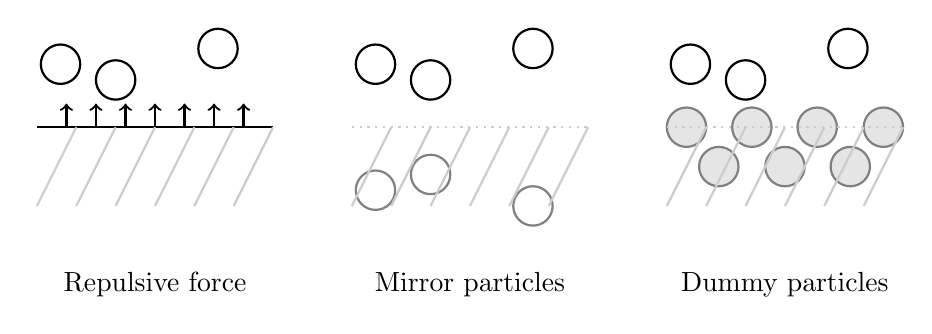
\begin{tikzpicture}[thick]
% Mathematical reflection
\draw (0.3,.8) circle (.25cm) node[pos=.5] (p0) {};
\draw (1,.6) circle (.25cm) node[pos=.5] (p1) {};
\draw (2.3,1) circle (.25cm) node[pos=.5] (p2) {};
\draw (0,0) -- (3,0);
\foreach \i in {1,...,6}{
	\draw[black!20] (.5*\i-.5,-1) -- (.5*\i,0);
}
% Forces
\foreach \i in {1,...,7}{
	\draw[->] (.375*\i,0) -- (.375*\i,.3);
}
\node at (1.5,-2) {Repulsive force};

% Mirror 
\draw (4.3,.8) circle (.25cm) node[pos=.5] (p0) {};
\draw (5,.6) circle (.25cm) node[pos=.5] (p1) {};
\draw (6.3,1) circle (.25cm) node[pos=.5] (p2) {};
\draw[black!50] (4.3,-.8) circle (.25cm) node[pos=.5] (mii1) {};
\draw[black!50] (5,-.6) circle (.25cm) node[pos=.5] (mii2) {};
\draw[black!50] (6.3,-1) circle (.25cm) node[pos=.5] (mii3) {};
\draw[black!20,dotted] (4,0) -- (7,0);
\foreach \i in {1,...,6}{
	\draw[black!20] (.5*\i-.5+4,-1) -- (.5*\i+4,0);
}
\node at (5.5,-2) {Mirror particles};

% Dummies
\draw[black!50,fill=black!10] (8.25,0) circle (.25cm) node[pos=.5] (d0) {};
\draw[black!50,fill=black!10] (9.08,0) circle (.25cm) node[pos=.5] (d1) {};
\draw[black!50,fill=black!10] (9.91,0) circle (.25cm) node[pos=.5] (d2) {};
\draw[black!50,fill=black!10] (10.75,0) circle (.25cm) node[pos=.5] (d3) {};
% second layer
\draw[black!50,fill=black!10] (8.66,-.5) circle (.25cm) node[pos=.5] (d4) {};
\draw[black!50,fill=black!10] (9.50,-.5) circle (.25cm) node[pos=.5] (d5) {};
\draw[black!50,fill=black!10] (10.33,-.5) circle (.25cm) node[pos=.5] (d6) {};
%\draw (1,-.25) circle (.25cm) node[pos=.5] (d4) {};
%normal parts
\draw (8.3,.8) circle (.25cm) node[pos=.5] (p0) {};
\draw (9,.6) circle (.25cm) node[pos=.5] (p1) {};
\draw (10.3,1) circle (.25cm) node[pos=.5] (p2) {};
\draw[dotted,black!20] (8,0) -- (11,0);
\foreach \i in {1,...,6}{
	\draw[black!20] (.5*\i-.5+8,-1) -- (.5*\i+8,0);
}
\node at (9.5,-2) {Dummy particles};
\end{tikzpicture}
\caption{Different boundaries condition methods}
\label{fig:SPH:boundaries}
\end{figure}

For this experiment, realistic boundaries conditions were needed. 
Several methods are possible with SPH we focused on the main ones, the repulsive wall, the mirror particles \cite{libersky1991smooth} and the dummies particles implementation \cite{adami2012generalized}. 
Those boundaries conditions implementation are presented in figure~\ref{fig:SPH:boundaries}.

For the current implementation, we used the dummies particles method.
The wall particles are just considered as normal particles, with specific equations, and their quantities are evolved during the run. 
The main difference is that their position does not evolve at the end of the step.
They are identified in the code with a specific type, provided during the data generation. 

\subsection{Astrophysics: neutron stars coalescence}

The final aim of our tests is to simulate astrophysical events. 
We are interested in one of the most important event recently discovered. 
Last year the Laser Interferometer Gravitational Wave, LIGO, detected the first gravitational wave generated by binary neutron stars merging \cite{abbott2017gw170817} and also more complexes event with Binary Black Holes coalescence in \cite{abbott2017gw170814}.


\subsubsection{Solving Lane-Emden Equation}

We need to determine the density function based on the radius. 

As we consider the star as a polytropic fluid, we use the equation of Lane-Emden which is a form of the Poisson equation: 

\begin{equation}\label{eq_LaneEmden}
  \frac{d^2\theta}{d \xi^2}+ \frac{2}{\xi}\frac{d\theta}{d\xi}+\theta^n = 0
\end{equation}

With $\xi$ and $\theta$ two dimensionless variables. 
There is only exact solutions for a polytropic index $n = 0.5$, $1$ and $2$.
In our work we use a polytropic index of $1$ which can correspond to a NS simulation.

For $n=1$ the solution of equation \ref{eq_LaneEmden} is: 

\begin{equation}
\theta(\xi)=\frac{sin(\xi)}{\xi}
\end{equation}

We note $\xi_1 = \pi$, the first value of $\xi$ as $\theta(\xi) = 0$.
$\theta(\xi)$ is also defined as: 
\begin{equation}
 \theta(\xi) = \Big(\frac{\rho(\xi)}{\rho_c}\Big)^{\frac{1}{n}}  = \frac{\rho(\xi)}{\rho_c}
\end{equation}

With $\rho_c$ the internal density of the star and $\rho$ the density at a determined radius. $\xi$ is defined as:  
$$ \xi = Ar = \sqrt{\frac{4\pi G}{K(n+1)}\rho_c^{(n-1)/n}} \times r = \sqrt{\frac{2\pi G}{K}}\times r \mbox{ (for } n=1 \mbox{)}$$

With $K$ a proportionality constant.

From the previous equations we can write the stellar radius $R$ as:
\begin{equation}
R = \sqrt{\frac{K(n+1)}{4\pi G}}\rho_c^{(1-n)/2}\xi_1 = \sqrt{ \frac{K}{2\pi G} } \times \xi_1
\end{equation} 

(We note that for $n=1$ the radius does not depend of the central density.)

If, for example, we use dimensionless units as $G=R=M=1$ (for the other results we use CGS with $G = 6.674 \times 10^{-8} cm^3g^{-1}s^{-2}$) 
We can compute K as: 
\begin{equation}
\label{eq:constant}
K = \frac{R^2  2 \pi G}{\xi_1^2}
\end{equation}

\begin{center}
\begin{tabular}{c|c|c|c|c|}
 & $NS_1$ & $NS_2$ & $NS_3$ & $NS_4$ \\ 
\hline 
Radius (cm) & $R=G=M=1$ & 1500000 & 1400000 & 960000 \\ 
\hline 
K & 0.636619 & 95598.00 & 83576.48 & 39156.94\\ 
\hline 
\end{tabular}
\end{center} 

Then we deduce the density function of $r$ as :

$$\rho(\xi) = \frac{sin(A\times r)}{A \times r} \times \rho_c \mbox{ with } A = \sqrt{\frac{2\pi G}{K}}
$$

As we know the total Mass $M$, the radius $R$ and the gravitational constant $G$ we can compute the central density as: 

$$ \rho_c = \frac{M A^3}{4 \pi (sin(AR)-ARcos(AR)) } $$

Then we normalize the results to fit $R = M = G = 1$: $K' = K/(R^2G) $, $m_i' = m_i/M $, $h_i' = h_i / R$, $\vec{x_i}' = \vec{x_i}/R$ 

\section{Conclusion}


%%%%%%%%%%%%%%%%%%%%%%%%%%%%%%%%%%%%%%%%%%%%%%%%%%%%%%%%%%%%%%%%%%%%%
%                                                                   %
% CHAPTER ONE, Computation wall                                     % 
%                                                                   %
%%%%%%%%%%%%%%%%%%%%%%%%%%%%%%%%%%%%%%%%%%%%%%%%%%%%%%%%%%%%%%%%%%%%%

%%%%%%%%%%%%%%%%%%%%%%%%%%%%%%%%%%%%%%%%%%%%%%%%%%%%%%%%%%%%%%%%%%%%%
%                                                                   %
%	CHAPTER TWO, HARDWARE IN HPC                                    %
%                                                                   %
%%%%%%%%%%%%%%%%%%%%%%%%%%%%%%%%%%%%%%%%%%%%%%%%%%%%%%%%%%%%%%%%%%%%%

\chapter{Hardware in HPC}

\section{Introduction}

Parallel models address most of the key points for application performance, but it may also depend on architectures hardware, which may influence how to consider the problems' resolution. 
Thus, the knowledge of hardware architecture is essential to reach performances through optimizations.
Even if the current software, API, framework or runtime already handle most of the optimizations, the last percents of performance gain are architecture dependent. 
In this chapter, we describe the most important devices architectures from classical processors, General Purpose Graphics Processing Units (GPGPUs), Field Programmable Gate Arrays (FPGAs) and Application-Specific Integrated Circuits (ASICs).
This study focuses on multi-core processors and GPUs as we based our tests on these devices. 

This chapter describes the architecture of some remarkable supercomputers. 
This comes with the description of interconnection network for the most used interconnection topologies. 

We choose to present the architectures in a chronological order following the models presented in the previous chapter - SISD, MIMD and SIMD/SIMT - and presenting the most recently released technologies.
We also present the optimizations of current technologies with the rise of parallelism and new types of memories.

\section{Early improvements of Von Neumann machine}
In this section, we present the different hardware evolution from the 1970s single core processors to modern multi-core and many-core architectures that are the milestones, and the basic units, for building supercomputers. 
We can observe the most important optimizations that are always implemented in the most recent machines: in/out of order processors, pre-fetching strategies, vectorization and the memory technologies breakthroughs. 

\subsection{Single core processors}
The first processors were developed in the 1970s and were built using a single computation core as described in the Von Neumann model. 
The single core processors were improved with many optimizations from the memory, the order of the instructions and the frequency to increase.

\subsubsection{Transistor shrink and frequency}
\index{Frequency}
Many new approaches to produce smaller transistors have been discovered.
Transistor sizes were about 10$\mu m$ in 1971 and reach 10$nm$ in current machines.
This allowed the constructors to add more transistors on the same die and build more complex ISA and features for the CPUs. 

In parallel of the shrink of transistors, the main feature for better performances with the single core architectures came from the frequency augmentation, the clock rate. 
As the clock rate increases, more operations can be performed on the core in the same amount of time. 
In the 1970s, the frequency was about 4 MHz allowing a maximum of 4 million of cycles per seconds. 
Nowadays, single cores can work at a frequency of 4GHz and even 5GHz performing billions of operations per cycles, but the following sections will demonstrate that due to power consumption and coding considerations, frequency is no longer used to improve performances. 

\subsubsection{In/Out-Of-Order execution} 
\index{In/Out of Order}
In-order-process is described in the previous chapter. 
This control unit fetches instructions and the operands from memory. 
The ALU then computes the operation before the final result is stored to the memory.

In this model, the time to perform an instruction is the accumulation of: instruction fetching + operand(s) fetching + \textit{computation} + result storage.
This time may be high regarding the use of the ALU for \textit{computation}, technically just one clock cycle. 
The idea of \textit{out-of-order} execution is to compute the instructions without following the Program Counter order. 
Indeed, for independent tasks, (indicated by dependency graphs) while the process fetches the next instruction data, the ALU can perform another operation with already available operands.
This leads to better usage of computational resources in the CPU, and thus better overall performances. 

\subsubsection{Vectorization} 
\index{Vectorization}
\index{Unrolling}
\index{Loop tiling}
Vector processors allow the instructions to be executed at the same time in a SIMD manner. 
If the same instruction is executed on coalescent data they can be executed in the same clock cycle. 
For an example, we can execute operations simultaneously on four to eight floats with a bus size of 128 or 256 bits.
This requires specific care for coding with \textit{unrolling} and \textit{loop tiling} to avoid bad behavior leading to poor performances and will be addressed later in this study.
The latest architectures vectorization imposes to slightly lower the frequency of processors. 

\index{Cray-1}
The Cray-1 supercomputer\cite{russell1978cray}, installed in 1975 in the Los Alamos National Laboratory, is a perfect example of vector processor supercomputer.
This supercomputer was designed by Seymour Cray, the founder of Cray Research, and was able to deliver up to 160 MFLOPS based on vector processor.
It was the fastest supercomputer in 1978 and due to its shape and price it was humorously called \textit{the world's most expansive love-seat}. 

\begin{figure}[t!]
\begin{center}
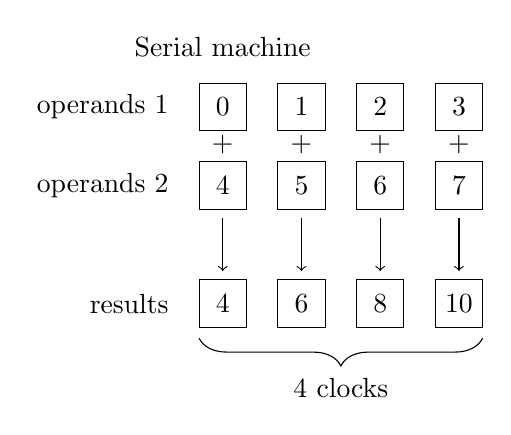
\begin{tikzpicture}
\foreach \x in {0,...,3}
{
	% Draw the rectangle 
	\draw (\x,0) rectangle (\x+.6,.6) node[pos=.5] (res\x) {
		\pgfmathparse{4+\x*2}
		\pgfmathprintnumber[precision=0]
        \pgfmathresult
    };
	\draw (\x,1.5) rectangle (\x+.6,2.1) node[pos=.5] (op2\x)  {
		\pgfmathparse{\x+4}
		\pgfmathprintnumber[precision=0]
        \pgfmathresult
    };
	\draw (\x,2.5) rectangle (\x+.6,3.1) node[pos=.5] (op1\x) {\x};
	% Draw the arrows for result
	\draw[->] ([yshift=-5pt]op2\x.south) -- ([yshift=5pt]res\x.north);
	\node at ([yshift=-7pt]op1\x.south) {$+$};
}
% add the arrow on top for clocks 
\draw [decorate,decoration={brace,amplitude=10pt,mirror,raise=4pt},yshift=0pt]
(0.,0) -- (3.6,0) node [black,midway,below,yshift=-15pt] {4 clocks};

\node[anchor=east] at ([xshift=-10pt]res0.west) {results};
\node[anchor=east] at ([xshift=-10pt]op10.west) {operands 1};
\node[anchor=east] at ([xshift=-10pt]op20.west) {operands 2};

\node[thick] at ([yshift=15pt]op10.north) {Serial machine};


% Add the name of architecture, classical serial 

% Add line name 
\end{tikzpicture}
\hspace{1cm}
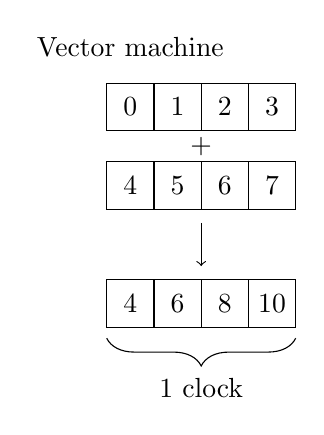
\begin{tikzpicture}
\foreach \x in {0,...,3}
{
	% Draw the rectangle 
	\draw (\x*.6,0) rectangle (\x*.6+.6,.6) node[pos=.5] (res\x) {
		\pgfmathparse{4+\x*2}
		\pgfmathprintnumber[precision=0]
        \pgfmathresult
    };
	\draw (\x*.6,1.5) rectangle (\x*.6+.6,2.1) node[pos=.5] (op2\x)  {
		\pgfmathparse{\x+4}
		\pgfmathprintnumber[precision=0]
        \pgfmathresult
    };
	\draw (\x*.6,2.5) rectangle (\x*.6+.6,3.1) node[pos=.5] (op1\x) {\x};
	% Draw the arrows for result
}

% Just onw arrow and plus sign 
\draw[->] ([yshift=-5pt]1.2,1.5) -- ([yshift=5pt]1.2,.6);
\node at ([yshift=-6pt]1.2,2.5) {$+$};

\draw [decorate,decoration={brace,amplitude=10pt,mirror,raise=4pt},yshift=0pt]
(0.,0) -- (2.4,0) node [black,midway,below,yshift=-15pt] {1 clock};

\node[thick] at ([yshift=15pt,]op10.north) {Vector machine};
\end{tikzpicture}
\end{center}
\caption{Vectorized processeur example on 4 integer addition: 128 bits wide bus}
\label{fig:2_HARD:vector}
\end{figure}

The behavior of vector machine is presented on figure~\ref{fig:2_HARD:vector} for a 16 bytes vector machine (4 integer of 4 bytes = 128 bits bus). 
We see on the left that performing the 4 operations requests in 4 cycle and, at the opposite, 1 cycle on the right with the vectorized machine.\\

Linked with the CPU optimizations, the memory optimizations also needs to be considered. 
Even if the ALU can perform billions of operations per second, it needs to be fed with data by fast transfers.

\subsubsection{Memory technology evolution}

The memories technologies optimizations address several aspects. 
The early 1980s saw the augmentation of bus size from 4 bits to presently 32 bits for single precision and 64 bits for double precision. 
Buses with 128 bits or 256 bits can also be used to allow vectorization presented just before. 

Different kind of technologies are considered in this study: the SRAM and DRAM. 

\paragraph{SRAM: }
\index{Static Random Access Memory}
The Static Random Access Memory (SRAM) is built using so called "flip-flop" circuits that can store data at any time time with no time lost in "refresh operations".
This kind of memory is very expensive to produce due to the number of transistors by memory cell, therefore, it is usually limited for small amounts of storage. 
The SRAM is mainly used for cache memory. 

\paragraph{DRAM: }
\index{Dynamic Random Access Memory}
The Dynamic Random Access Memory (DRAM) is based on transistors and capacitors to store binary information.
This memory is less expensive to produce but needs to be refreshed at a determined frequency, otherwise the data are lost. 
This refresh step is a read-write operation on the whole memory at a specific frequency. 
There are several sub-categories of DRAM used in different device depending on the way the bus are used with Single Data Rate (SDR), Double Data Rate (DDR) and Quad Data Rates (QDR). 
The number of data carried can vary from one times to four times, but the limitation of those products is the price and are constantly rising. 

The latest more efficient memory is the 3D memory.
This is a stack of the different components instead of usual 2D distribution.
This memory, 3D XPoint, was created by Intel and Micron Technology and announced in July 2015. 
It can now be find in the NVIDIA GPUs, named 3D-stacked in P100 and V100.

\subsubsection{Cache memory: }
\index{Cache mechanism}
\begin{figure}[t!]
\centering
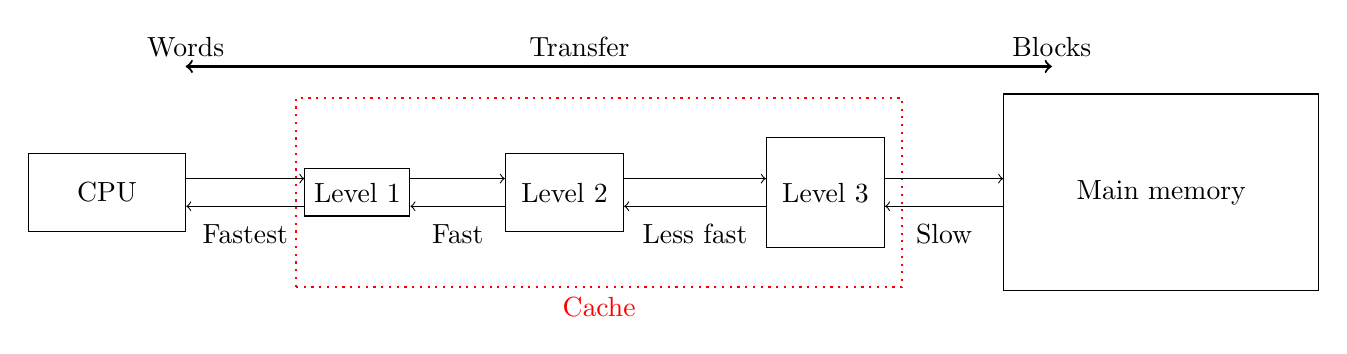
\begin{tikzpicture}
\node (rect) at (0,0) [draw,minimum width=2cm,minimum height=1cm] (cpu) {CPU};
\node[right = 1.5cm of cpu] (rect) [draw,minimum width=1cm,minimum height=.6cm] (cache_1) {Level 1};
\node[right = 1.2cm of cache_1] (rect) [draw,minimum width=1.5cm,minimum height=1cm] (cache_2) {Level 2};
\node[right = 1.8cm of cache_2] (rect) [draw,minimum width=1.5cm,minimum height=1.4cm] (cache_3) {Level 3};
\node[right = 1.5cm of cache_3] (rect) [draw,minimum width=4cm,minimum height=2.5cm] (ram) {Main memory};

\draw[thick,draw,red,dotted] (2.4,-1.2) rectangle  (10.1,1.2);
\node[below,red,thick] at (6.25,-1.2) {Cache}; 
% links 
\draw[->] ([yshift=5pt]cpu.east) -- ([yshift=5pt]cache_1.west);
\draw[<-] ([yshift=-5pt]cpu.east) -- ([yshift=-5pt]cache_1.west) node[midway,yshift=-10pt] {Fastest};

\draw[->] ([yshift=5pt]cache_1.east) -- ([yshift=5pt]cache_2.west);
\draw[<-] ([yshift=-5pt]cache_1.east) -- ([yshift=-5pt]cache_2.west) node[midway,yshift=-10pt] {Fast};

\draw[->] ([yshift=5pt]cache_2.east) -- ([yshift=5pt]cache_3.west);
\draw[<-] ([yshift=-5pt]cache_2.east) -- ([yshift=-5pt]cache_3.west) node[midway,yshift=-10pt] {Less fast};

\draw[->] ([yshift=5pt]cache_3.east) -- ([yshift=5pt]ram.west);
\draw[<-] ([yshift=-5pt]cache_3.east) -- ([yshift=-5pt]ram.west) node[midway,yshift=-10pt] {Slow};

\draw[<->,thick] (1,1.6) node[above]{Words} -- (12,1.6) node[above] {Blocks};
\node[above] at (6,1.6) {Transfer}; 
\end{tikzpicture}
\caption{Cache memory technology on three levels L1, L2 and L3}
\label{fig:2_HARD:caches}
\end{figure}
Cache is a memory mechanism that is useful to consider when targeting performance. 
The main idea of cache technology is presented on figure~\ref{fig:2_HARD:caches}.
This memory is built hierarchically over several levels. 
L1 is the closest to the CPU followed by L2 with generally no levels past L3 except on specific architectures. 
When looking for data, the CPU first checks if the data is present in the L1 cache, otherwise it will look in L2 and L3 to get the data to higher level. 
From the main memory to the L3 cache \textit{blocks} are exchanged, by chunks. 
With levels L1 and L2, lines of information are exchanged, usually referred to as \textit{words}.
This is based on the idea that if a data is used, it shall be used again in the near future.
Many cache architectures exist: direct, associative, fully associative, etc. 
Cache-hits occur when the data required is present in cache versus a cache-miss occurs when it has to be retrieved from lower levels or main memory. 
The ratio of cache-miss has to be kept low in a program in order to reach performance, and the impact may be very high.

\subsubsection{Pre-fetching} 
\index{Pre-fetching}
Pre-fecthing was developed based on memory optimization and especially for the cache.
When data are not available in L1 cache, it has to be moved from either L2 to L1 or L3 to L2 to L1 or in the worst case from RAM to L3 to L2 to L1. 
Pre-fecthing technology is a way to, knowing the next instructions operands, pre-fetch the data in closer cache before the instruction is decoded. 
The pre-fetch can either be hardware or software implemented and can concern data and even instructions.

\subsection{Multi-CPU servers and multi-core processors}
Around the beginning of the 2000s, the limitations of single core processors were very important. 
The frequency was already high and requested more power consumption causing more heat dissipation. 
The first solution to this problem was to provide multi-CPU devices, embedding several CPU on the same motherboard and allowing them to share memory. 
The evolution of the mono-core is the multi-core having several processing units on the same die allowed more optimization inside the die and combining all the advantages of single core processors.
But by embedding each CPU, the function and units required consume $n$ times more energy with cumulate heat effects.
Thus, unable to answer the constant augmentation of computational power needed for research and HPC, IBM was the first company to create a multi-core CPU in 2001, the Power4. 

Compared to the core inside multi-CPU, multi-core CPU shared one of the material (L3 caches, buses, etc.) and are implemented on the same due; this allows to reach the same CPU performances with less transistors and less power consumption, avoiding most of the heating issues. 

\begin{figure}
\centering 
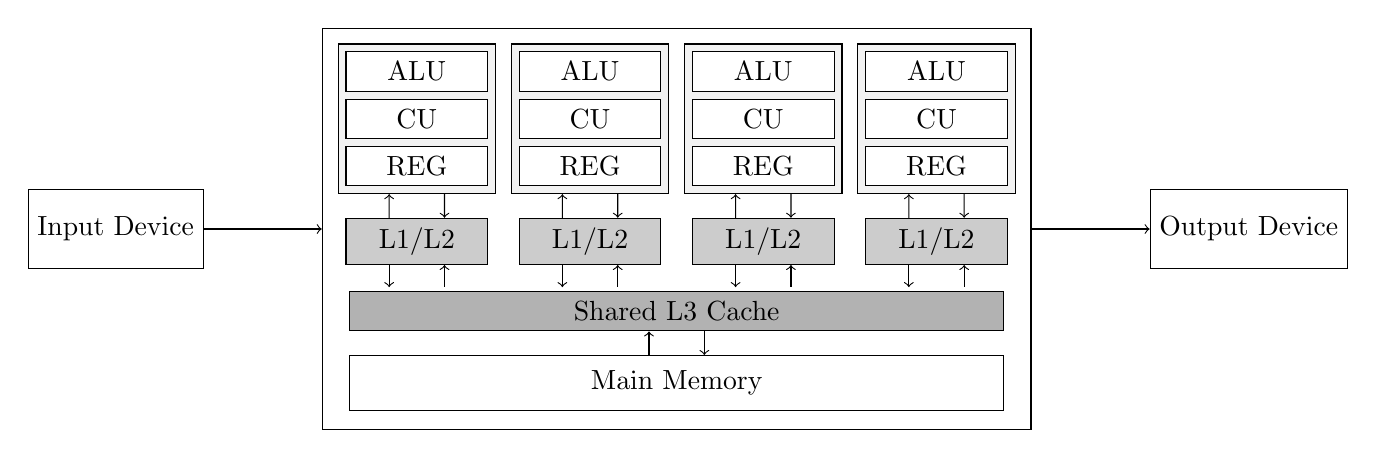
\begin{tikzpicture}

\node (rect) at (0,0) [draw,minimum width=2cm,minimum height=1cm] (input) {Input Device};

\node[right = 1.5cm of input] (rect) [draw,minimum width=9cm,minimum height=5.1cm] (machine) {};

\node[fill=black!30] (rect) at ([yshift=-3.6cm]machine.north) [draw,minimum width=8.3cm,minimum height=.5cm] (l3) {Shared L3 Cache};

\foreach \x in {0,...,3}{
	\node[anchor=north west,fill=black!5] (rect) at ([yshift=-.2cm,xshift=\x*2.2cm+.2cm]machine.north west) [draw,minimum width=2cm,minimum height=1.9cm] (cpu\x) {};

	\node[anchor=north west,fill=white] (rect) at ([yshift=-.1cm,xshift=.1cm]cpu\x.north west) [draw,minimum width=1.8cm,minimum height=.5cm] {ALU};
	\node[anchor=north west,fill=white] (rect) at ([yshift=-.7cm,xshift=.1cm]cpu\x.north west) [draw,minimum width=1.8cm,minimum height=.5cm] {CU};
	\node[anchor=north west,fill=white] (rect) at ([yshift=-1.3cm,xshift=.1cm]cpu\x.north west) [draw,minimum width=1.8cm,minimum height=.5cm] {REG};
	% Cache memory
	\node[anchor=north west,fill=black!20] (rect) at ([yshift=-.3cm,xshift=.1cm]cpu\x.south west) [draw,minimum width=1.8cm,minimum height=.5cm] (l1\x) {L1/L2};
	% Arriw 
	\draw[->] ([xshift=-10pt]l1\x.north) -- ([xshift=-10pt]cpu\x.south);
	\draw[<-] ([xshift=10pt]l1\x.north) -- ([xshift=10pt]cpu\x.south);
	% Arrow to L3
	\draw[->] ([xshift=-10pt]l1\x.south) -- ([xshift=-10pt,yshift=-8pt]l1\x.south);
	\draw[<-] ([xshift=10pt]l1\x.south) -- ([xshift=10pt,yshift=-8pt]l1\x.south);

	%\draw[<-] ([xshift=10pt]l1\x.south) |- (l3.north);
	
}


\node[below = .3cm of l3] (rect) [draw,minimum width=8.3cm,minimum height=.7cm] (mem) {Main Memory};

\node[right = 1.5cm of machine] (rect) [draw,minimum width=2cm,minimum height=1cm] (output) {Output Device};

\draw[->] ([xshift=-10pt]mem.north) -- ([xshift=-10pt]l3.south);
\draw[<-] ([xshift=10pt]mem.north) -- ([xshift=10pt]l3.south);

\draw[->] (input.east) -- (machine.west);
\draw[->] (machine.east) -- (output.west);

\end{tikzpicture}
\caption{Multi-core CPU with 4 cores based on Von Neumann Model}
\label{fig:2_HARD:von_neumann_model_multi-core}
\end{figure}

This architecture is presented on figure~\ref{fig:2_HARD:von_neumann_model_multi-core}.
The main memory is now shared between the cores. 
The registers and L1/L2 cache are the same but a L3 layer is added to the cache, and consistency has to be maintained over all the cores. 
If a process modifies a data in the memory this information has to be spread over all the other users of this data, even in their local cache. 

We note here that in current language the CPU, as describe in the Von Neumann model, is also the name of the die containing several cores. 
This is the architecture of most of current processors and these multi-cores provide two to 32 cores in most cases. 
Thus, the multi-core CPU are called "Host" and the attached accelerators are called "Devices".

\section{21th century architectures}
After years of development and research on hardware for Computer Science and specifically HPC, we present here the latest and best technologies to produce efficient and general-purpose supercomputers.

We present the latest architectures with multi-core, many-core and specific processors, and the most famous manufacturers. 

\subsection{Multi-core implementations}
The most world spread architecture in public and high performance computing is the multi-core processors. 
Most present-day accelerators require a classical processor to offload tasks and data on it. 

We start this presentation from the most popular processors in HPC world from the Intel company ones. 
We also present ARM which is a different multi-core architecture based on RISC instructions set.

\subsubsection{Intel}
\index{Intel}
Intel was created in 1968 by a chemist and a physicist, Gordon E. Moore and Robert Noyce, in Mountain View, California. 
Processors today are typically from Intel, the world leader which equips around 90\% of the supercomputers (November 2017 TOP500 list).

In 2007, Intel adopted a production model called the "Tick-Tock", presented on figure~\ref{fig:1_HPC:intel_tick_tock}.
\begin{figure}[t!]
\begin{center}
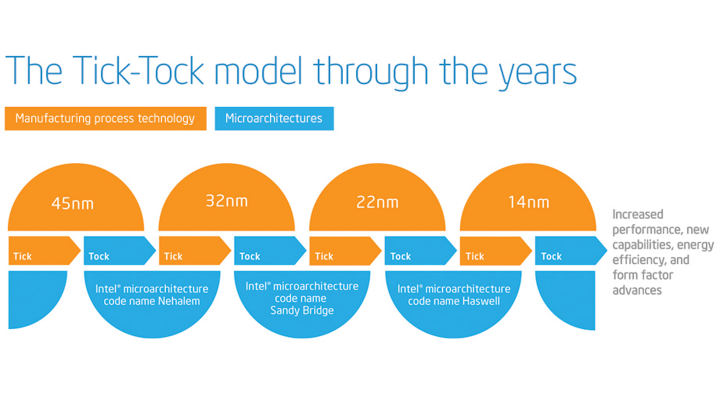
\includegraphics[width=.8\textwidth]{\locpath/figures/chap1/intel_tick_tock.png}
\caption{Intel Tick-Tock model}
\label{fig:1_HPC:intel_tick_tock}
\end{center}
\end{figure}
Since the creation of the Tick-Tock model, it always followed the same fashion: a new manufacturing technology, such as shrinking the chip with better engraving, on a "Tick" followed by a "Tock" which delivers a new micro-architecture.
The Intel processors for HPC are called Xeon and feature ECC memory, higher number of cores, large RAM support, large cache-memory, Hyper-threading, etc. 
Compared to desktop processors, their performances are of a different magnitude.
Intel has given every new processor a code name. 
The last generations are chronologically called Westemere (2011), Sandy Bridge (2012), Ivy Bridge(2013), Haswell (2014), Broadwell (2015), Skylake (2015) and Kaby lake (2016). 

Kaby Lake, the last architecture provided, does not exactly fit the typical "Tick-Tock" process because it is just based on optimizations of the Skylake architecture. 
The Kaby Lake is produced like Skylake with an engraving of 14 nm.
The Tick-Tock model appears to be hard to maintain due to the difficulties to engrave in less than 10 nm with quantum tunneling. 
This leads to using larger many-cores architecture and the bases of the next supercomputer evolutions, the road-map to hybrid models. 

\paragraph{Hyper-threading}
\index{Hyper-threading}
Another specificity of Intel Xeon processors is Hyper-threading (HT). 
This technology makes a single physical processing unit (core) appearing as two logical ones for the user's level.
In fact, a processor embedding 8 cores appears as a 16 cores for user. 
Adding more computation per node can technically allow the cores to switch context when data are fetched from the memory using the processor 100\% during all the computation. 
Multiple studies have been published on HT from Intel itself~\cite{marr2002hyperthreading} to independent researchers~\cite{bononi2006exploring,leng2002empirical}.
This optimization does not fit to all the cases of applications and can be disabled for normal use of the processors in the context of general purpose HPC architectures.

\subsubsection{ARM}
\index{Advanced RISC architecture}
Back in the 1980s, ARM stood for Acorn RISC Machine in reference to the first company to implement this kind of architecture, Acorn Computers. 
This company later changed the name to Advanced RISC Machine (ARM). 
ARM is a specific kind of processors based on RISC architecture as its ISA, despite usual processors using CISC.
The downside of CISC machines are they are difficult to create and they require way more transistor and thus more energy to work. 
The ISA from the RISC is simpler and requires multiple many transistors to operate and thus a smaller silicon area on the die.
Therefore, the energy required and the heat dissipated is less important. 
It becomes easier to create massively parallel processors based on ARM. 
On the other hand, simple ISA imposes more work on the source code compilation to fit the simple architecture. 
This makes the instructions sources longer, and therefore, more single instructions to execute. 

The ARM company provides several versions of ARM processors named Cortex-A7X (2015), Cortex-A5X (2014) and Cortex-A3X (2015) featured for highest-performances, for balancing performances and efficiency or for less power consumption, respectively. 

\index{Mont-Blanc project}
The new ARMv8 architecture starts to provide the tools to target HPC context~\cite{rico2017arm}.
The European approach towards energy efficient HPC, Mont-Blanc project\footnote{http://montblanc-project.eu/}, already constructs ARM based supercomputers. 
The exascale project in Horizon 2020 this project focuses on using ARM-based systems for HPC with many famous contributors, such as Atos/Bull as a project coordinator, ARM, French Alternative Energies and Atomic Energy Commission (CEA), Barcelona Supercomputing Center (BSC), etc.
The project is separated into several steps to finally reach Exascale near 2020. 
The last step, Mont-Blanc 3, is about to work on a pre-Exascale prototype powered by Cavium’s ThunderX2 ARM chip based on 64-bits ARMv8.

\subsection{Intel Xeon Phi}
\index{Xeon Phi}
Another specific HPC product from Intel is the Xeon Phi. 
This device can be considered as a Host or Device/Accelerator machine. 
Intel describes it as "a bootable host processor that delivers massive parallelism and vectorization".
This architecture embed multiple multi-cores processors interconnected and is called Intel's Many Integrated Core (MIC).
We placed this architecture here because it provides hundreds of conventional computation core but the program counter is not shared between them. 
It does not fit in the many-core architecture but is a step in the multi-core one. 
This is the technology on which Intel bases its Exascale machines. 

The architectures names are Knights Ferry, Knights Corner and Knight Landing~\cite{sodani2016knights}. 
The last architecture, Knight Hill, was recently canceled by Intel due to low performances and to focus the Xeon Phi for Exascale.
The main advantage of this architecture compared to GPGPUs is the x86 compatibility of the embedded cores and the fact this device can boot and use to drive other accelerators. 
They also feature more complex operations and handle double precision natively.

\subsection{Many-core architecture, SIMT execution model}
\index{Single Instruction Multiple Threads}
Several architectures can be defined as many-cores and follow the SIMD model from Flynn taxonomy.
These devices integrate thousands of cores that are usually control by fewer control units. 
We can consider these cores as "simpler" since they have to work synchronously and under the coordination of a control unit.
Some devices are specific like the Xeon Phi of Intel, integrating a hundred of regular processor cores which can work independently. 

\subsubsection{GPU}
\index{Graphics Processing Unit}
A CPU can usually have two to 32 computation cores that can operate on different instruction streams, but the SIMT architecture of the GPU is slightly different. 
The cores are grouped and must share the same instruction at the same clock time, but different groups can have their own instructions. 

\begin{figure}
\begin{center}
% classical processor
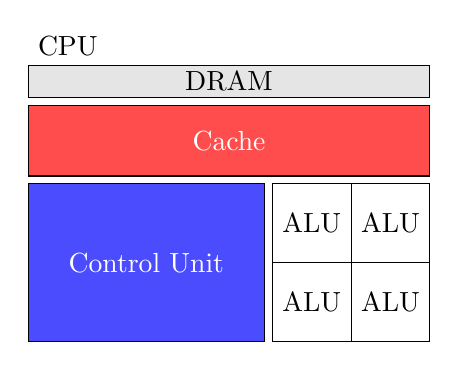
\begin{tikzpicture}
% ALUs
\foreach \x in {3,...,4}
	\foreach \y in {0,...,1}
		\draw[] (\x+.1,\y) rectangle (\x+1.1,\y+1) node[pos=.5] {ALU};
% Control Unit
\draw[fill=blue!70] (0,0) rectangle (3,2) node[pos=.5,text=white] {Control Unit};
%Cache
\draw[fill=red!70] (0,2.1) rectangle (5.1,3) node[pos=.5,text=white] {Cache};
% DRAM
\draw[fill=black!10] (0,3.1) rectangle (5.1,3.5) node[pos=.5] {DRAM};
%Name 
\node[yshift=7pt,anchor=west] at (0,3.5) {CPU};
\end{tikzpicture}
\hspace{1cm}
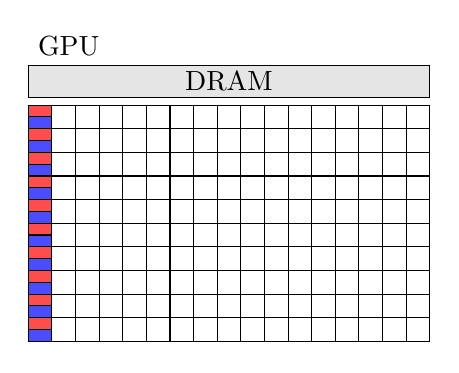
\begin{tikzpicture}
% ALUs
\foreach \y in {0,...,9}
{
	\draw[fill=blue!70] (0,\y * .3) rectangle (.3,\y * .3 + .15) node[pos=.5] {};
	\draw[fill=red!70] (0,\y * .3 + .15) rectangle (.3,\y * .3 + .3) node[pos=.5] {};
	\foreach \x in {1,...,16}
		\draw[] (\x*.3,\y*.3) rectangle (\x *.3+.3,\y*.3+.3) node[pos=.5] {};
}
% DRAM
\draw[fill=black!10] (0,3.1) rectangle (5.1,3.5) node[pos=.5] {DRAM};
% Name 
\node[yshift=7pt,anchor=west] at (0,3.5) {GPU};
\end{tikzpicture}
\end{center}
\caption{Multi-core versus Many-core architecture, case of GPUs}
\label{fig:2_HARD:gpu}
\end{figure}

Figure~\ref{fig:2_HARD:gpu} present the vision between CPU and GPU processors. 
We note in this figure that the usual topology with the ALU lined up in front of their control unit and shared cache memory. 
Every ALU has its own memory and registers to operate local computations. 

These devices are called General Purpose Graphics Processing Units (GPGPUs). 
They are derivative from classical GPUs used for graphical purpose.
Pioneers show that GPGPUs can be use efficiently for classical scientific computations.
The vendor provides then specific GPU for general purpose computing.  
We present here the two main companies providing GPGPUs for HPC world: NVIDIA and AMD.

\paragraph{NVIDIA GPU architecture}
\index{NVIDIA}
The NVIDIA company was founded in April 1993 in Santa Clara, Carolina by three persons, one being the current CEO, Jensen Huang.
The company name originated from \textit{invidia} the Latin word for Envy and vision for graphical rendering. 

NVIDIA is known as the pioneer in graphics, cryptocurrency, portable devices, and now Artificial Intelligence (IA) and appears to be even the creator of the name "GPU".
NVIDIA's GPUs, inspired from visualization and gaming at a first glance, are available as a dedicated device for HPC purpose since the company released the brand named \textit{Tesla}. 
The public GPUs can also be used for dedicated computation, but does not feature ECC memory, double precision or special functions/FFT cores. 
The different versions of the architecture are named following famous physicists, chronologically: Tesla, Fermi, Kepler, Maxwell, Pascal and Volta.

\index{K20Xm}
We describe here the Kepler brand GPU and more specifically the K20Xm GPU on which we based our study. 
\begin{figure}
\centering
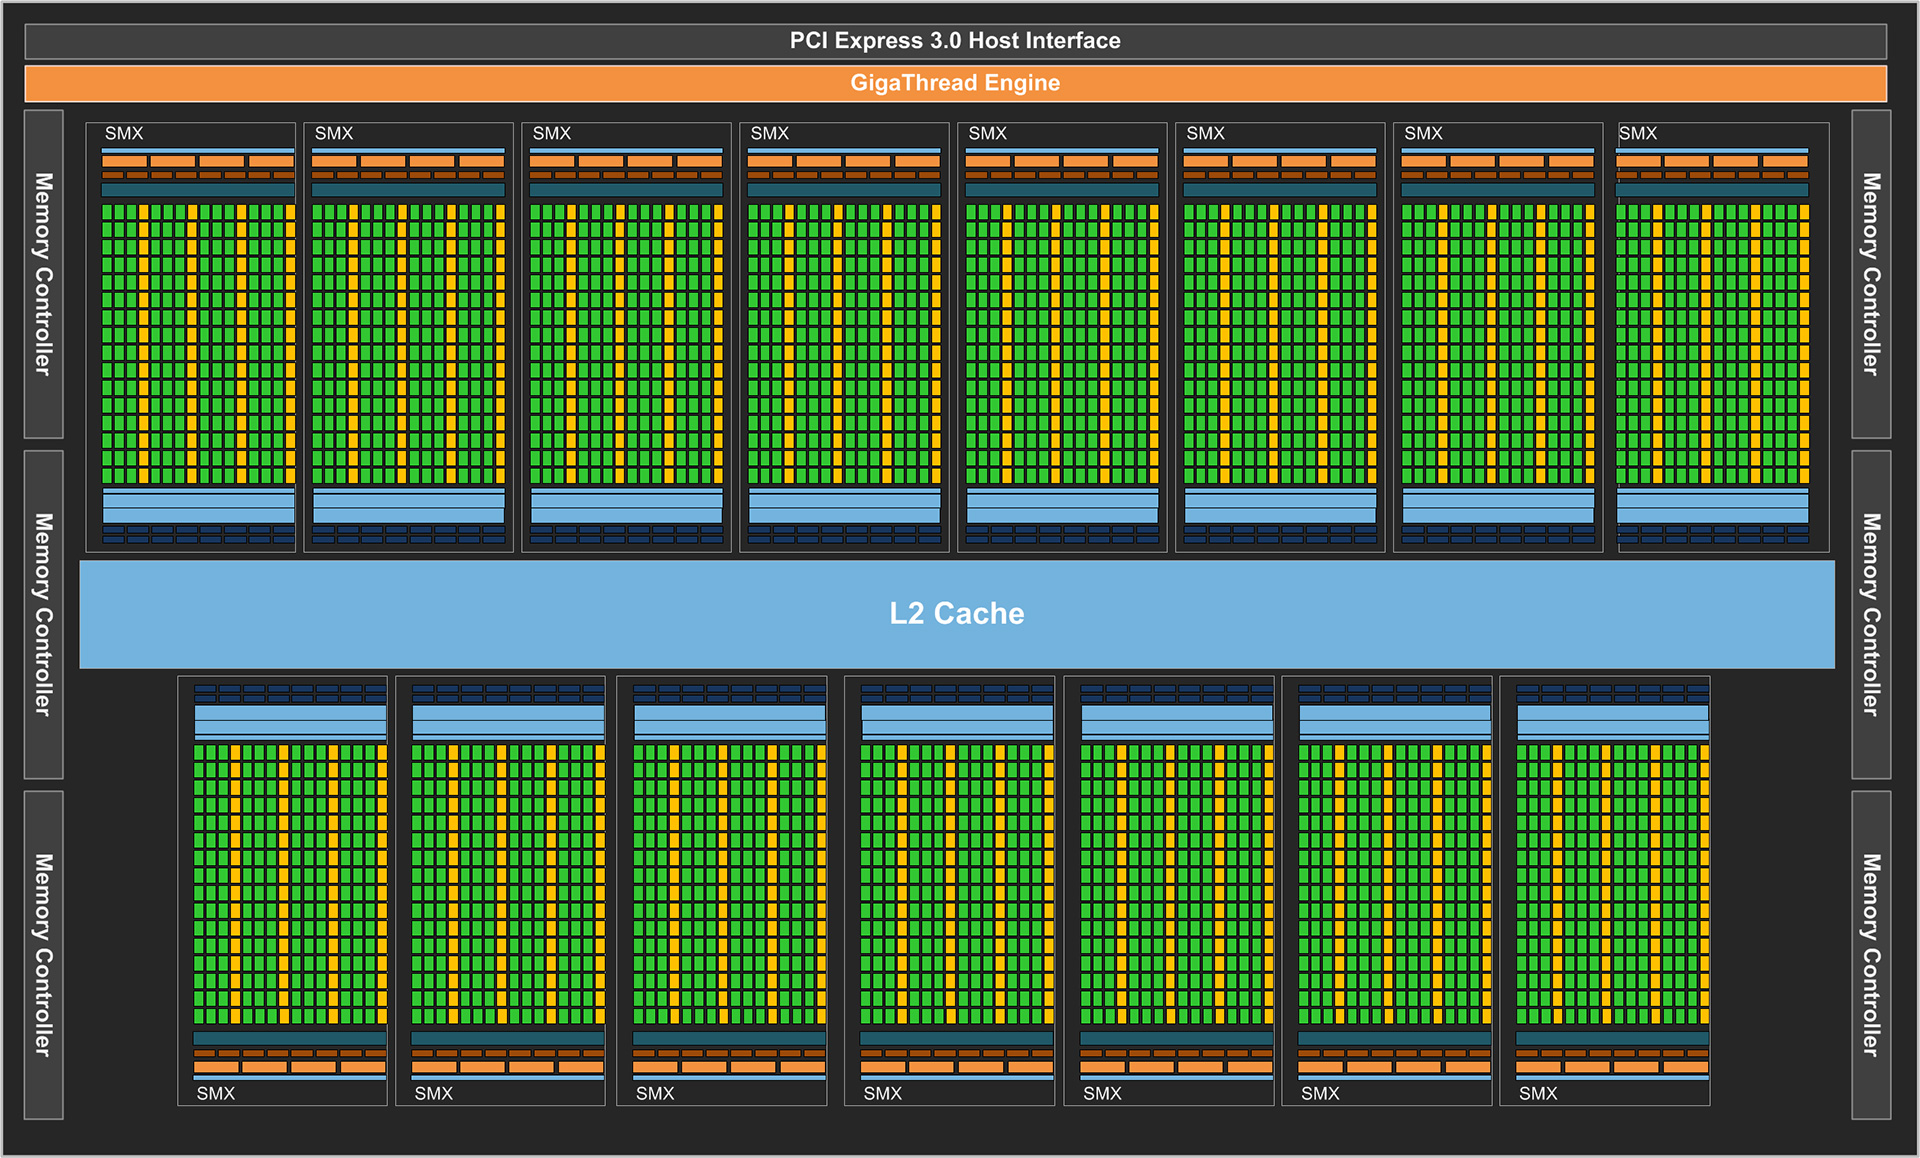
\includegraphics[width=\textwidth]{\locpath/figures/chap1/kepler_architecture.jpeg}
\caption{NVIDIA Tesla Kepler architecture. Single-precision in green and double-precision in yellow}
\label{fig:2_HARD:kepler_arch}
\end{figure}
This NVIDIA Tesla Kepler GPU is based on the GK110 graphics processor describes in the white-paper\cite{nvidia2012nvidias} on 28nm process.
The figure~\ref{fig:2_HARD:kepler_arch} is a representation of the physical elements of this graphics processor. 
The K20X comes in active and passive cooling mode with K20Xc and K20Xm, respectively.
This GPU embeds 2688 CUDA cores distributed in 14 SMX (we note that GK110 normally provides 15 SMX but only 14 are present on the K20X).
In this model each SMX contains 192 single precisions cores, 64 double precision cores, 32 special function units and 32 load/store units.
In a SMX the memory provides 65536 32-bits registers, 64 KB of shared memory L1 cache, 48 KB of read-only cache
The L2 cache is 1546 KB shared by the SMX for a total of 6 GB of memory adding the DRAM.
The whole memory is protected using Single‐Error Correct Double‐Error Detect (SECDED) ECC code.
The power consumption is estimated to 225 W.
This GPGPU is expected to produce 1.31 TFLOPS for double-precision and 3.95 TFLOPS of single-precision.

\paragraph{AMD}
\index{AMD}
Another company is providing GPUs for HPC, Advanced Micro Devices (AMD). 
In front of the huge success of NVIDIA GPU that leads from far the HPC market, it is hard for AMD to find a place for its GPGPUs, the FirePro, in HPC. 
The FirePro is targeted using a language near CUDA, not held by a single company by NVIDIA like CUDA, called OpenCL. 
An interesting creation of AMD is the Accelerated Processing Units (APUs) which embedded the processor and the GPU on the same die since 2011. 
This solution allows them to target the same memory. 

In the race to market and performances, AMD found an accord with Intel to provide dies featuring Intel processor, AMD GPU and common HBM memory. 
The project is call Kaby Lake-G and announced it would be available in the first semester of 2018 for public, not HPC itself. 

\subsubsection{PEZY}
\index{PEZY}
Another many-core architecture only appeared in the last benchmarks. 
The PEZY Super Computer 2, PEZY-SC2, is the third many-core microprocessor developed by the company PEZY. 
The three first machines ranked in the GREEN500 list are accelerator using this many-core die. 
We also note that in the November 2017 list, the fourth supercomputer, Gyoukou, is also powered by PEZY-SC2 cards.

\subsection{Other architectures}
Numerous architectures have not been presented here because they are out of scope of this study. 
We present here two technologies we have encountered in our researches and that may be tomorrow solution for Exascale in HPC. 
\subsubsection{FPGA}
\index{Field Programmable Gates Array}
Field Programmable Gates Array (FPGA) are devices that can be reprogram to fit the needs of the user after their construction.
The leader were historically Altera with the Stratix, Arria and Cyclone FPGAs, which is now part of Intel. 
With the FPGAs, the users have access to the hardware and can design their own circuits. 
Currently, FPGA can be targeted with OpenCL programming language. 
The arrival of Intel in this market assures the best hopes for HPC version of FPGAs. 
The main gap for users is the circuit building that can be designed for specific needs but may be hard to setup. 
\subsubsection{ASIC}
\index{Application Specified Integrated Circuits}
Application Specified Integrated Circuits are dedicated device construct for on purpose. 
An example of ASIC is the Gravity Pipe (GRAPE) which is dedicated to compute gravitation given mass and positions.
Google leads the way for ASIC and recently created its dedicated devices to boost AI bots.
ASIC may be found in some optimized communication devices, such as fast interconnection network in HPC.  

\section{Distributed architectures}

The technologies presented in previous part is the milestone of supercomputers. 
They are used together in a whole system to create machine delivering incredible computational power.

\subsection{Architecture of a supercomputer}
From the hardware described before, we can create the architecture of a cluster from the smallest unit, cores, nodes, to the whole system.

\begin{description}[noitemsep,nolistsep]
\item[Core:] A core is the smallest unit in our devices. 
It refers to the Von Neumann model in case of core with ALU and CU. 
We can separate cores from CPU to GPU, the first one able to be independent whereas the second ones working together and share the same program counter. 
\item[Socket/Host:] A socket is mistakenly called a CPU in current language. 
It is, for multi-cores sockets, composed of several cores. 
The name Host comes from the Host-Device architecture using accelerators. 
\item[Accelerators/Devices:] Accelerators are devices that, when attached to the Host, provide additional computational power. 
We can identify them as GPUs, FPGAs, ASICs, etc. 
A socket can have access to one or more accelerators and can also share the accelerator usage. 
\item[Computation node: ] The next layer of our HPC system is the computation node, which is a group of several sockets and accelerators sharing memory;
\item[Rack: ] A rack is a set of computation nodes, generally in vertical stack. 
It may also include specific nodes dedicated to the network or the Input/Output.
\item[Interconnection: ] The nodes are grouped together with hard wire connection following a specific interconnection topology with very high bandwidth.
\item[System/Cluster/Supercomputer] The cluster group several racks though an interconnection network.
\end{description}

An interconnect technology is required in order to connect nodes together and allow distributed programming. 
Interconnection networks are the way the nodes of a cluster are connected together. 

\subsection{Interconnection topologies}
\index{Interconnect}
Several topologies exist from point to point to multi-dimensional torus.
%
\begin{figure}[t!]
\centering
\resizebox {.14\columnwidth} {!} {
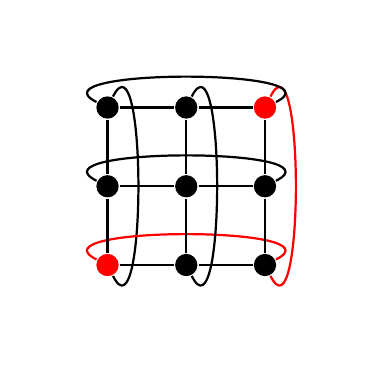
\begin{tikzpicture}[thick,inner sep=0.1cm]
	\node [fill,circle,red] (node 1000) at (0,0) {};
	\node [fill,circle] (node 1001) at (1,0) {};
	\node [fill,circle] (node 1002) at (2,0) {};
	\node [fill,circle] (node 1003) at (0,1) {};
	\node [fill,circle] (node 1004) at (1,1) {};
	\node [fill,circle] (node 1005) at (2,1) {};
	\node [fill,circle] (node 1006) at (0,2) {};
	\node [fill,circle] (node 1007) at (1,2) {};
	\node [fill,circle,red] (node 1008) at (2,2) {};
	
	\draw (node 1000)
							         .. controls +(0.500000,-1.000000)
							                 and +(0.500000,1.000000)
							         .. (node 1006);
	\draw[red] (node 1000)
							         .. controls +(-1.000000,0.500000)
							                 and +(1.000000,0.500000)
							         .. (node 1002);
	\draw (node 1000) -- (node 1001);
	\draw (node 1000) -- (node 1003);
	\draw (node 1001) -- (node 1004);
	\draw (node 1001)
							         .. controls +(0.500000,-1.000000)
							                 and +(0.500000,1.000000)
							         .. (node 1007);
	\draw (node 1002) -- (node 1005);
	\draw (node 1002) -- (node 1001);
	\draw[red] (node 1002)
							         .. controls +(0.500000,-1.000000)
							                 and +(0.500000,1.000000)
							         .. (node 1008);
	
	\draw (node 1003)
							         .. controls +(-1.000000,0.500000)
							                 and +(1.000000,0.500000)
							         .. (node 1005);
	\draw (node 1003) -- (node 1006);
	\draw (node 1003) -- (node 1004);
	\draw (node 1004) -- (node 1005);
	\draw (node 1004) -- (node 1007);
	\draw (node 1005) -- (node 1008);
	\draw (node 1006)
							         .. controls +(-1.000000,0.500000)
							                 and +(1.000000,0.500000)
							         .. (node 1008);
	\draw (node 1006) -- (node 1007);
	\draw (node 1007) -- (node 1008);
\end{tikzpicture}
}
%\vspace{1cm}
\resizebox {.34\columnwidth} {!} {
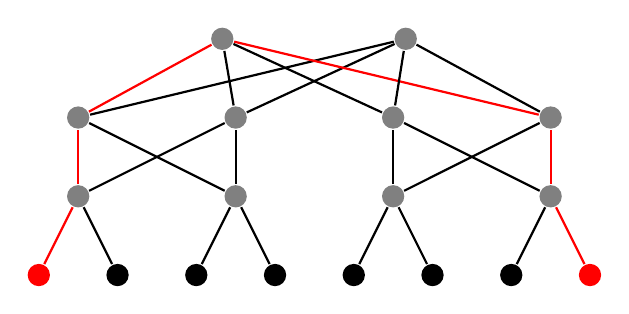
\begin{tikzpicture}[thick,inner sep=0.1cm]
	
	\node [fill,circle,red] (node a) at (0,0) {};
	\node [fill,circle] (node b) at (1,0) {};
	\node [fill,circle] (node c) at (2,0) {};
	\node [fill,circle] (node d) at (3,0) {};
	\node [fill,circle] (node e) at (4,0) {};
	\node [fill,circle] (node f) at (5,0) {};
	\node [fill,circle] (node g) at (6,0) {};
	\node [fill,circle,red] (node h) at (7,0) {};

	\node [fill,circle,black!50] (node a0) at (0.5,1) {};
	\node [fill,circle,black!50] (node a1) at (2.5,1) {};
	\node [fill,circle,black!50] (node a2) at (4.5,1) {};
	\node [fill,circle,black!50] (node a3) at (6.5,1) {};
	\node [fill,circle,black!50] (node a4) at (0.5,2) {};
	\node [fill,circle,black!50] (node a5) at (2.5,2) {};
	\node [fill,circle,black!50] (node a6) at (4.5,2) {};
	\node [fill,circle,black!50] (node a7) at (6.5,2) {};

	\node [fill,circle,black!50] (node n0) at (2.33,3) {};
	\node [fill,circle,black!50] (node n1) at (4.66,3) {};

	\draw[red] (node a) -- (node a0);
	\draw (node b) -- (node a0);
	\draw (node c) -- (node a1);
	\draw (node d) -- (node a1);
	\draw (node e) -- (node a2);
	\draw (node f) -- (node a2);
	\draw (node g) -- (node a3);
	\draw[red] (node h) -- (node a3);

	\draw[red] (node a0) -- (node a4);
	\draw (node a0) -- (node a5);
	\draw (node a1) -- (node a4);
	\draw (node a1) -- (node a5);
	\draw (node a2) -- (node a6);
	\draw (node a2) -- (node a7);
	\draw (node a3) -- (node a6);
	\draw[red] (node a3) -- (node a7);

	\draw[red] (node n0) -- (node a4);
	\draw (node n1) -- (node a5);
	\draw (node n0) -- (node a5);
	\draw (node n1) -- (node a4);
	\draw (node n0) -- (node a6);
	\draw (node n1) -- (node a7);
	\draw[red] (node n0) -- (node a7);
	\draw (node n1) -- (node a6);
\end{tikzpicture}
}
%\caption{Torus and 4-ary tree}
%\end{figure}
%\begin{figure}
\resizebox {.24\columnwidth} {!} {
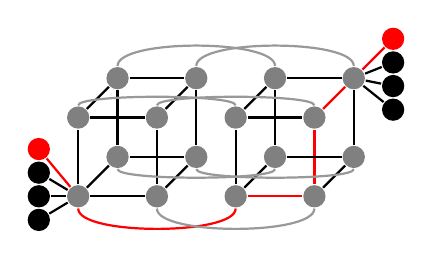
\begin{tikzpicture}[thick,inner sep=0.1cm]
	
	\node [fill,circle,black!50] (node a0) at (0,0) {};
	\node [fill,circle,black!50] (node b0) at (1,0) {};
	\node [fill,circle,black!50] (node c0) at (0,1) {};
	\node [fill,circle,black!50] (node d0) at (1,1) {};
	\node [fill,circle,black!50] (node e0) at (0.5,0.5) {};
	\node [fill,circle,black!50] (node f0) at (1.5,0.5) {};
	\node [fill,circle,black!50] (node g0) at (0.5,1.5) {};
	\node [fill,circle,black!50] (node h0) at (1.5,1.5) {};

	\node [fill,circle,black!50] (node a1) at (2,0) {};
	\node [fill,circle,black!50] (node b1) at (3,0) {};
	\node [fill,circle,black!50] (node c1) at (2,1) {};
	\node [fill,circle,black!50] (node d1) at (3,1) {};
	\node [fill,circle,black!50] (node e1) at (2.5,0.5) {};
	\node [fill,circle,black!50] (node f1) at (3.5,0.5) {};
	\node [fill,circle,black!50] (node g1) at (2.5,1.5) {};
	\node [fill,circle,black!50] (node h1) at (3.5,1.5) {};

	\node [fill,circle,red] (node cn0) at (4,2.) {};
	\node [fill,circle] (node cn1) at (4,1.7) {};
	\node [fill,circle] (node cn2) at (4,1.4) {};
	\node [fill,circle] (node cn3) at (4,1.1) {};

	\node [fill,circle] (node cn4) at (-0.5,-0.3) {};
	\node [fill,circle] (node cn5) at (-0.5,0.0) {};
	\node [fill,circle] (node cn6) at (-0.5,0.3) {};
	\node [fill,circle,red] (node cn7) at (-0.5,0.6) {};


	\draw (node a0) -- (node b0);
	\draw (node b0) -- (node d0);
	\draw (node c0) -- (node d0);
	\draw (node a0) -- (node c0);
	\draw (node e0) -- (node f0);
	\draw (node f0) -- (node h0);
	\draw (node g0) -- (node h0);
	\draw (node e0) -- (node g0);

	\draw (node a0) -- (node e0);
	\draw (node b0) -- (node f0);
	\draw (node c0) -- (node g0);
	\draw (node d0) -- (node h0);

	\draw[red] (node a1) -- (node b1);
	\draw[red] (node b1) -- (node d1);
	\draw (node c1) -- (node d1);
	\draw (node a1) -- (node c1);
	\draw (node e1) -- (node f1);
	\draw (node f1) -- (node h1);
	\draw (node g1) -- (node h1);
	\draw (node e1) -- (node g1);

	\draw (node a1) -- (node e1);
	\draw (node b1) -- (node f1);
	\draw (node c1) -- (node g1);
	\draw[red] (node d1) -- (node h1);

	\draw[red] (node cn0) -- (node h1);
	\draw (node cn1) -- (node h1);
	\draw (node cn2) -- (node h1);
	\draw (node cn3) -- (node h1);
	\draw (node cn4) -- (node a0);
	\draw (node cn5) -- (node a0);
	\draw (node cn6) -- (node a0);
	\draw[red] (node cn7) -- (node a0);

	%\draw (node a0) -- (node a1);
	\draw[red] (node a0)
		        .. controls +(0.,-0.500000)
		                 and +(0.,-0.500000)
		        .. (node a1);
	\draw[black!40] (node b0) 
				.. controls +(0.,-0.500000)
		                 and +(0.,-0.500000)
		        .. (node b1);
	\draw[black!40] (node c0) 
				.. controls +(0.,0.300000)
		                 and +(0.,0.300000)
		        ..  (node c1);
	\draw[black!40] (node d0) 
				.. controls +(0.,0.300000)
		                 and +(0.,0.300000)
		        ..  (node d1);
	\draw[black!40] (node e0) 
				.. controls +(0.,-0.300000)
		                 and +(0.,-0.300000)
		        ..  (node e1);
	\draw[black!40] (node f0) 
				.. controls +(0.,-0.300000)
		                 and +(0.,-0.300000)
		        ..  (node f1);
	\draw[black!40] (node g0) 
				.. controls +(0.,0.500000)
		                 and +(0.,0.500000)
		        ..  (node g1);
	\draw[black!40] (node h0) 
				.. controls +(0.,0.500000)
		                 and +(0.,0.500000)
		        ..  (node h1);
\end{tikzpicture}
}
%\hspace{1cm}
\resizebox {.24\columnwidth} {!} {
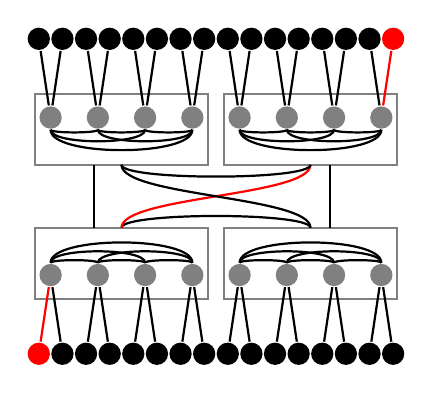
\begin{tikzpicture}[thick,inner sep=0.1cm]
	\node [fill,circle,black!50] (node a00) at (0.45,1) {};
	\node [fill,circle,black!50] (node a01) at (1.05,1) {};
	\node [fill,circle,black!50] (node a02) at (1.65,1) {};
	\node [fill,circle,black!50] (node a03) at (2.25,1) {};
	\node [fill,circle,red] (node n01) at (0.3,0) {};
	\node [fill,circle] (node n02) at (0.6,0) {};
	\node [fill,circle] (node n03) at (0.9,0) {};
	\node [fill,circle] (node n04) at (1.2,0) {};
	\node [fill,circle] (node n05) at (1.5,0) {};
	\node [fill,circle] (node n06) at (1.8,0) {};
	\node [fill,circle] (node n07) at (2.1,0) {};
	\node [fill,circle] (node n08) at (2.4,0) {};

	\node [fill,circle,black!50] (node a10) at (2.85,1) {};
	\node [fill,circle,black!50] (node a11) at (3.45,1) {};
	\node [fill,circle,black!50] (node a12) at (4.05,1) {};
	\node [fill,circle,black!50] (node a13) at (4.65,1) {};
	\node [fill,circle] (node n11) at (2.7,0) {};
	\node [fill,circle] (node n12) at (3,0) {};
	\node [fill,circle] (node n13) at (3.3,0) {};
	\node [fill,circle] (node n14) at (3.6,0) {};
	\node [fill,circle] (node n15) at (3.9,0) {};
	\node [fill,circle] (node n16) at (4.2,0) {};
	\node [fill,circle] (node n17) at (4.5,0) {};
	\node [fill,circle] (node n18) at (4.8,0) {};

	\node [fill,circle,black!50] (node a20) at (0.45,3) {};
	\node [fill,circle,black!50] (node a21) at (1.05,3) {};
	\node [fill,circle,black!50] (node a22) at (1.65,3) {};
	\node [fill,circle,black!50] (node a23) at (2.25,3) {};
	\node [fill,circle] (node n21) at (0.3,4) {};
	\node [fill,circle] (node n22) at (0.6,4) {};
	\node [fill,circle] (node n23) at (0.9,4) {};
	\node [fill,circle] (node n24) at (1.2,4) {};
	\node [fill,circle] (node n25) at (1.5,4) {};
	\node [fill,circle] (node n26) at (1.8,4) {};
	\node [fill,circle] (node n27) at (2.1,4) {};
	\node [fill,circle] (node n28) at (2.4,4) {};

	\node [fill,circle,black!50] (node a30) at (2.85,3) {};
	\node [fill,circle,black!50] (node a31) at (3.45,3) {};
	\node [fill,circle,black!50] (node a32) at (4.05,3) {};
	\node [fill,circle,black!50] (node a33) at (4.65,3) {};
	\node [fill,circle] (node n31) at (2.7,4) {};
	\node [fill,circle] (node n32) at (3,4) {};
	\node [fill,circle] (node n33) at (3.3,4) {};
	\node [fill,circle] (node n34) at (3.6,4) {};
	\node [fill,circle] (node n35) at (3.9,4) {};
	\node [fill,circle] (node n36) at (4.2,4) {};
	\node [fill,circle] (node n37) at (4.5,4) {};
	\node [fill,circle,red] (node n38) at (4.8,4) {};

	\draw[black!50] (2.65,2.4) rectangle (4.85,3.3);
	\draw[black!50] (0.25,2.4) rectangle (2.45,3.3);

	\draw[black!50] (2.65,0.7) rectangle (4.85,1.6);
	\draw[black!50] (0.25,0.7) rectangle (2.45,1.6);

	\draw (1.35,1.6)
	.. controls +(0.,0.2)
	    and +(0.,0.2)
	..  (3.75,1.6); 

	\draw[red] (1.35,1.6)
	.. controls +(0.,0.4)
	    and +(0.,-0.4)
	..  (3.75,2.4); 
	%\draw (1.35,1.6) -- (3.75,2.4);
	\draw (3.75,1.6)
	.. controls +(0.,0.4)
	    and +(0.,-0.4)
	..  (1.35,2.4); 
	%\draw (3.75,1.6) -- (1.35,2.4);

	\draw (1.,1.6) -- (1.,2.4);
	\draw (4.,1.6) -- (4.,2.4);

	\draw (1.35,2.4)
	.. controls +(0.,-0.2)
	    and +(0.,-0.2)
	..  (3.75,2.4); 


	\draw[red] (node n01) -- (node a00);
	\draw (node n02) -- (node a00);
	\draw (node n03) -- (node a01);
	\draw (node n04) -- (node a01);
	\draw (node n05) -- (node a02);
	\draw (node n06) -- (node a02);
	\draw (node n07) -- (node a03);
	\draw (node n08) -- (node a03);

	\draw (node n11) -- (node a10);
	\draw (node n12) -- (node a10);
	\draw (node n13) -- (node a11);
	\draw (node n14) -- (node a11);
	\draw (node n15) -- (node a12);
	\draw (node n16) -- (node a12);
	\draw (node n17) -- (node a13);
	\draw (node n18) -- (node a13);

	\draw (node n21) -- (node a20);
	\draw (node n22) -- (node a20);
	\draw (node n23) -- (node a21);
	\draw (node n24) -- (node a21);
	\draw (node n25) -- (node a22);
	\draw (node n26) -- (node a22);
	\draw (node n27) -- (node a23);
	\draw (node n28) -- (node a23);

	\draw (node n31) -- (node a30);
	\draw (node n32) -- (node a30);
	\draw (node n33) -- (node a31);
	\draw (node n34) -- (node a31);
	\draw (node n35) -- (node a32);
	\draw (node n36) -- (node a32);
	\draw (node n37) -- (node a33);
	\draw[red] (node n38) -- (node a33);

	\draw (node a00) 
	.. controls +(0.,0.2)
	    and +(0.,0.2)
	..  (node a01);
	\draw (node a00) 
	.. controls +(0.,0.35)
	    and +(0.,0.35)
	..  (node a02);
	\draw (node a00) 
	.. controls +(0.,0.5)
	    and +(0.,0.5)
	..  (node a03);
	\draw (node a01) 
	.. controls +(0.,0.2)
	    and +(0.,0.2)
	..  (node a02);
	\draw (node a01) 
	.. controls +(0.,0.35)
	    and +(0.,0.35)
	..  (node a03);
	\draw (node a02) 
	.. controls +(0.,0.2)
	    and +(0.,0.2)
	..  (node a03);

	\draw (node a10) 
	.. controls +(0.,0.2)
	    and +(0.,0.2)
	..  (node a11);
	\draw (node a10) 
	.. controls +(0.,0.35)
	    and +(0.,0.35)
	..  (node a12);
	\draw (node a10) 
	.. controls +(0.,0.5)
	    and +(0.,0.5)
	..  (node a13);
	\draw (node a11) 
	.. controls +(0.,0.2)
	    and +(0.,0.2)
	..  (node a12);
	\draw (node a11) 
	.. controls +(0.,0.35)
	    and +(0.,0.35)
	..  (node a13);
	\draw (node a12) 
	.. controls +(0.,0.2)
	    and +(0.,0.2)
	..  (node a13);

	\draw (node a20) 
	.. controls +(0.,-0.2)
	    and +(0.,-0.2)
	..  (node a21);
	\draw (node a20) 
	.. controls +(0.,-0.35)
	    and +(0.,-0.35)
	..  (node a22);
	\draw (node a20) 
	.. controls +(0.,-0.5)
	    and +(0.,-0.5)
	..  (node a23);
	\draw (node a21) 
	.. controls +(0.,-0.2)
	    and +(0.,-0.2)
	..  (node a22);
	\draw (node a21) 
	.. controls +(0.,-0.35)
	    and +(0.,-0.35)
	..  (node a23);
	\draw (node a22) 
	.. controls +(0.,-0.2)
	    and +(0.,-0.2)
	..  (node a23);

	\draw (node a30) 
	.. controls +(0.,-0.2)
	    and +(0.,-0.2)
	..  (node a31);
	\draw (node a30) 
	.. controls +(0.,-0.35)
	    and +(0.,-0.35)
	..  (node a32);
	\draw (node a30) 
	.. controls +(0.,-0.5)
	    and +(0.,-0.5)
	..  (node a33);
	\draw (node a31) 
	.. controls +(0.,-0.2)
	    and +(0.,-0.2)
	..  (node a32);
	\draw (node a31) 
	.. controls +(0.,-0.35)
	    and +(0.,-0.35)
	..  (node a33);
	\draw (node a32) 
	.. controls +(0.,-0.2)
	    and +(0.,-0.2)
	..  (node a33);
\end{tikzpicture}
}
\caption{Torus, Fat-Tree, HyperX, DragonFly}
\label{fig:1_HPC:topology}
\end{figure}
%
The figure~\ref{fig:1_HPC:topology} is a representation of famous topologies. 
Each interconnect technology has its own specificity. 
These networks take in account the number of nodes to interconnect and the targeted bandwidth/budget.
Several declination of each network are not detailed here. 
The Mesh and the Torus are used as a basis in lower layers of others more complex interconnection networks. 
A perfect example is the supercomputer called K-Computer describe in the next section.
The Fat Tree presented here is a k-ary Fat Tree, the higher the position in the tree, the more connections are found and with a bandwidth being important. 
The nodes are available as the leaves, on the middle level we find the switches and on top the routers. 
This is the topology of the ROMEO supercomputer we used for our tests. 
Another topology, HyperX\cite{ahn2009hyperx}, is based on Hyper-Cube.
The DragonFly\cite{kim2008technology} interconnect is recent, 2008, and is used in modern day supercomputers.

InfiniBand (IB)\index{Infiniband} is the most widespread technology used for interconnection with different kind of bandwidth presented in figure~\ref{fig:1_HPC:infiniband}.
It provides high bandwidth and small latency and companies such as Intel, Mellanox, etc. provide directly adapters and switches specifically for IB. 

\begin{table}[t!]
\begin{center}
\[\arraycolsep=0.pt\def\arraystretch{1.2}
\begin{tabular}{| l | l | l || l | l | l | }
\hline
\textbf{Name} & \textbf{Gbs} & \textbf{Year} & \textbf{Name} & \textbf{Gbs} & \textbf{Year} \\
\hline
\hline
Single DR & 2.5 & 2003 & Enhanced DR & 25 & 2014 \\
\hline
Double DR & 5 & 2005 & Highg DR & 50 & 2017 \\
\hline
Quad DR & 10 & 2007 & Next DR & 100 & 2020 \\
\hline
Fourth DR & 14 & 2011 & & &  \\
\hline
\end{tabular}
\]
\caption{InfiniBand technologies name, year and bandwidth}
\label{fig:1_HPC:infiniband}
\end{center}
\end{table}

Unfortunately, this augmentation of clock rate is not sustainable due to the energy required and the heat generated by the running component. 
Another idea originated in the 19th century with the first multi-core processors. 


\subsection{Remarkable supercomputers}
The TOP500\footnote{\url{https://www.top500.org}} is the reference benchmarks for the world rank supercomputers. 
This benchmark is based on the LINPACK and aim to solve a dense system of linear equations.
Most of the TOP10 machines have specific architectures and, of course, the most efficient ones. 
In this section, we describe several supercomputers about their interconnect, processors and specific accelerators. 

\subsubsection{Sunway Taihulight}
\index{Sunway Taihulight}
Sunway Taihulight is the third Chinese supercomputer to be ranked in the first position of the TOP500 list, in November 2017. 
A recent report from Jack J. Dongarra, a figure in HPC, decrypted the architecture of this supercomputer\cite{dongarra2016report}. 
The most interesting point is the conception of this machine, completely done in China. 
The Sunway CPUs were designed and built in China by the Shanghai High Performance IC Design Center. 

\begin{figure}[t!]
\centering
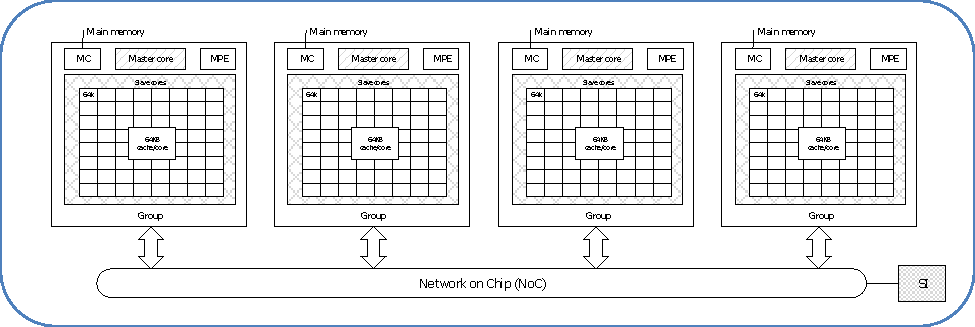
\includegraphics[scale=1]{\locpath/figures/Chap1/report_sunway_CPE}
\caption{Sunway Taihulight node architecture from \textit{Report on the Sunway TaihuLight System}, Jack Dongarra, June 24, 2016.}
\label{fig:chap1_report_sunway_CPE}
\end{figure}

The SW26010, a many core architecture processor, features 260 cores based on RISC architecture and a specific conception, depicted on figure~\ref{fig:chap1_report_sunway_CPE}. 
The processor is composed of the master core, a Memory Controller (MC) and a Management Processing Element (MPE) that manages the Computing Processing Elements (CPE), which are the slaves’ cores. 

The interconnect network is called Sunway Network and is connected using Mellanox Host Channel Adapter (HCA) and switches. 
This is a five-level interconnect going through computing nodes, computing board, super-nodes and cabinets to the complete system.
For the latest TOP500 list, from November 2017, the total memory is 1.31 PB and the number of cores available is 10,649,600.
The peak performance is 125.4 PFLOPS but the Linpack is only 93 PFLOPS which is 74.16\% of theoretic efficiency. 

\subsubsection{Piz Daint}
\index{Piz Daint}
The supercomputer of the CSCS, Swiss National Supercomputing Center, is currently ranked second on the November 2017 TOP500 list. 
This GPUs accelerated supercomputer is a most powerful representative of GPU hybrid acceleration and is the most powerful European supercomputer. 
This supercomputer is composed of 4761 hybrids and 1210 multi-core nodes. 
\index{NVIDIA}
There are hybrids nodes embedding an Intel Xeon E5-2690v3 and an NVIDIA Tesla Pascal P100 GPGPU. 
The interconnect is based on a Dragonfly network topology and Cray Aries routing and communications ASICs. 
The peak performance is 25.326 TFLOPS using only the hybrid nodes with Linpack generating 19.590 TFLOPS.
The low power consumption ranks Piz Daint as tenth in the November 2017 GREEN500.

\subsubsection{K-Computer}
\index{K-Computer}
The K-Computer was the top 1 supercomputer of the 2011 TOP500. 
The TOFU interconnect network makes the K-Computer unique~\cite{ajima2009tofu} and stands for TOrus FUsion.
\begin{figure}[t!]
\begin{center}
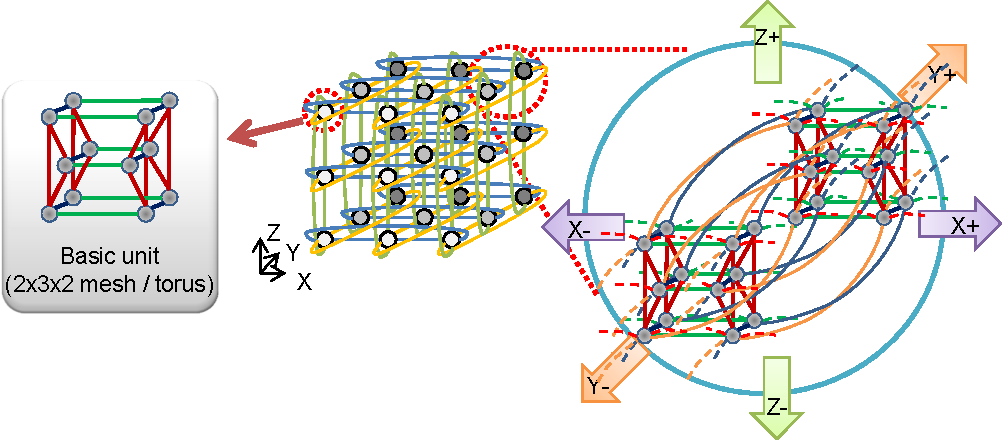
\includegraphics[width=\textwidth]{\locpath/figures/chap1/6d_torus}
\end{center}
\caption{TOFU Interconnect schematic from \textit{The K-Computer: System Overview}, Atsuya Uno, SC11}
\label{fig:1_HPC:tofu}
\end{figure}
\index{Interconnection}
This interconnect presented in figure~\ref{fig:1_HPC:tofu} mixes a 6D Mesh/Torus interconnect.
The basic units are based on a mesh and are interconnected together in a three-dimensional torus. 
In this configuration, each node can access to its 12 neighbors directly. 
It also provide a fault tolerant network with many routes to reach distant node. 

%\todo{AJouter MIRA/SEQUOIA pour paler de IBM, pour le Graph500 = meilleurs supercomputers}
%\todo{Parler de CRAY ?}
\subsubsection{Sequoia/Mira}
\index{IBM BlueGene}
The Sequoia supercomputer was ranked first on the 2012 TOP500 list. 
It is based on BlueGene from IBM.
The BlueGene project made up to three main architectures with BlueGene/L, BlueGene/P and BlueGene/Q.
It is very interesting to note the BlueGene architecture because 15 machine utilizing this architecture were in the top 200 in the last GRAPH500 list in November 2017.
The algorithm used on these supercomputers will be our basis in the Part II regarding our implementation of the GRAPH500 benchmark.

\section{ROMEO Supercomputer}
\index{ROMEO Supercomputer}
The ROMEO supercomputer center is the computation center of the Champagne-Ardenne region in France. 
Hosted since 2002 by the University of Reims Champagne-Ardenne, this so called meso-center (Medium size HPC center) is used for HPC in theoretic research and domain science like applied mathematics, physics, biophysics and chemistry. 

This project is supported by Europe, National Fundings, Grand-Est region and Reims Metropole. 
It aims to host research and production codes of the region for industrial, research and academics purposes. 

We are currently working on the fourth version of ROMEO, last updated in 2013. 
As many of our tests in this study have been done on this machine, we will carefully describe its architecture. 

This supercomputer was ranked 151st in the TOP500 and fifth in the GREEN500 list. 

\subsection{ROMEO hardware architecture}
\label{sec:part1_ROMEO}
ROMEO is a Bull/Atos supercomputer composed of 130 BullX R421 computing nodes. 

\index{K20Xm}
Each node is composed of two processors Intel Ivy Bridge 8 cores @ 2,6 GHz. 
Each processor has access to 16 GB of memory for a total of 32 GB per node, the total memory of 4.160 TB. 
Each processor is linked, using PCIe-v3, to an NVIDIA Tesla K20Xm GPGPU. 
This cluster provides then 260 processors for a total of 2080 CPU cores and 260 GPGPU providing 698880 GPU cores. 
The computation nodes are interconnected with an Infiniband QDR non-blocking network structured as a FatTree. 
The Infiniband is a QDR providing 10 GB/s. 

The storage for users is 57 TB and the cluster also provide 195 GB of Lustre and 88TB of parallel scratch file-system. 

In addition to the 130 computations nodes, the cluster provides a visualization node NVIDIA GRID with two K2 cards and 250GB of DDR3 RAM. 
The old machine, renamed Clovis, is also available but does not features GPUs. 

The supercomputer supports MPI with GPU Aware and GPUDirect. 

ROMEO is based on the Slurm\footnote{\url{https://slurm.schedmd.com/}} workload manager for node distribution among the users. 
This manager allows different usage of the cluster with classical reservation-submission or more asynchronous computation with best-effort. 
We developed advantages of both submissions systems in Part II. 

\subsection{New ROMEO supercomputer, June 2018}

In June 2018 a new version of the supercomputer ROMEO will be installed at the University of Reims Champagne Ardenne. 
This project intents to feature a supercomputer ranked around 250th in TOP500. 
It is a renewed partnership between ATOS/BULL and NVIDIA. 

The new ROMEO will feature 115 computation nodes with a total of 3220 CPU cores. 
The technology selected is the BULL \textit{Sequana} with its high energy saving, BXI network technology, NVLink support for GPUs and the density of the cluster. 
Each node will provide a Skylake 6132 CPU with 14 cores with a maximum frequency of 2.6GHz.

Two different types of node are present: 
\begin{itemize}[noitemsep,nolistsep]
\item[-] 70 of the with 4 GPUs and 96GB of RAM featuring a total of 280 Pascal P100 SMX2 GPUs.
\item[-] 45 last generation Intel CPUs with 192GB of memory per CPU. 
\end{itemize}

The machine will feature up to 15.3TB of global memory. 

The aim is to provide a performance of 964.6 TFLOPS in LINPACK and to be present in several TOP500 lists with a starting position around 232th or 297th. 

\section{Conclusion}

In this chapter, we reviewed the most important modern day hardware architectures and technologies. 
In order to use the driver or API in the most efficient way, we need to keep in mind the way the data and instructions are proceed by the machine. 

Efficiency is based on computation power, but also communications, we showed different interconnection topologies and their specificities. 
We present perfect use cases of the technologies in the current top ranked systems.
We show that every architecture is unique in its construction and justify the optimization work dedicated to reach performance. 

We determine from the new technologies presented here that supercomputers are moving toward hybrids architectures featuring multi-core processors accelerated by one or more devices such as many-core architectures. 
The Exascale supercomputer of 2020 will be shaped using hybrid architectures and they represent the best of nowadays technology for purpose of HPC this day and age. 
Combining CPU and GPUs or FPGA on the same die and sharing the same memory space may also be another solution.


%%%%%%%%%%%%%%%%%%%%%%%%%%%%%%%%%%%%%%%%%%%%%%%%%%%%%%%%%%%%%%%%%%%%%
%                                                                   %
% CHAPTER ONE, Communication WALL                                   % 
%                                                                   %
%%%%%%%%%%%%%%%%%%%%%%%%%%%%%%%%%%%%%%%%%%%%%%%%%%%%%%%%%%%%%%%%%%%%%

\documentclass[11pt,a4paper]{book}
\usepackage[utf8]{inputenc}
\usepackage[english]{babel}
\usepackage{amsmath}
\usepackage{amsfonts}
\usepackage{amssymb}
\usepackage{graphicx}
\usepackage{url}
\usepackage{python}
\usepackage{algpseudocode,algorithm}
\usepackage{tikz}
\usepackage{todonotes}
\usepackage{makeidx}
\usepackage{enumitem}
\usepackage{array}
\usepackage{makecell}


\newcommand{\locpath}{..}

\usepackage[left=2.5cm,right=2.5cm,top=2cm,bottom=2.5cm]{geometry}

% Thesis title
%\title{Energy Efficiency, Exascale and Complex Systems}
\title{Vers l'Exascale: Des Probl\`emes Th\'eoriques aux Probl\`emes Appliqu\'es\\
The Way to Exascale: From Theorics to Applied Problems}
% Author
\author{Julien Loiseau}
% Date 
\date{\today}

\makeindex

\begin{document}
\setcounter{chapter}{2}

\documentclass[11pt,a4paper]{book}
\usepackage[utf8]{inputenc}
\usepackage[english]{babel}
\usepackage{amsmath}
\usepackage{amsfonts}
\usepackage{amssymb}
\usepackage{graphicx}
\usepackage{url}
\usepackage{python}
\usepackage{algpseudocode,algorithm}
\usepackage{tikz}
\usepackage{todonotes}
\usepackage{makeidx}
\usepackage{enumitem}
\usepackage{array}
\usepackage{makecell}


\newcommand{\locpath}{..}

\usepackage[left=2.5cm,right=2.5cm,top=2cm,bottom=2.5cm]{geometry}

% Thesis title
%\title{Energy Efficiency, Exascale and Complex Systems}
\title{Vers l'Exascale: Des Probl\`emes Th\'eoriques aux Probl\`emes Appliqu\'es\\
The Way to Exascale: From Theorics to Applied Problems}
% Author
\author{Julien Loiseau}
% Date 
\date{\today}

\makeindex

\begin{document}
\setcounter{chapter}{2}

\input{\locpath/chapters/part1/chap3}

\bibliographystyle{alpha}
\bibliography{\locpath/biblio/biblio_langford,\locpath/biblio/biblio_graph,\locpath/biblio/biblio_sph,\locpath/biblio/biblio_hpc}

\end{document}


\bibliographystyle{alpha}
\bibliography{\locpath/biblio/biblio_langford,\locpath/biblio/biblio_graph,\locpath/biblio/biblio_sph,\locpath/biblio/biblio_hpc}

\end{document}


\section*{Conclusion}
% Chapter Three 
\part{Application}

\chapter*{Introduction}
The first part presented the tools needed to understand and target performance in HPC. 
The second part presented a metric showing the benefit of accelerators, in this case GPUs, over classical GPU in two contexts: irregular computation and irregular communication/memory behaviors.
We showed that the accelerators gave a real advantage on those two problems and allows us to push the limits.

In order to conclude this study and our metric we decided to target another irregular behavior problem embedding both computation/communication/memory wall behavior. 
In order to show how accelerators handle real world problems, we searched for an application fulfilling our needs. 
Our choose fell on the Smoothed Particle Hydrodynamics problem applied to fluid and astrophysics. 
The first version of this application was developed during a 2 months internship at the Los Alamos National Laboratory from the FleCSI framework.

In this part we first present the Smoothed Particle Hydrodynamics method from a physical point of view and making a parallel with the computer science problems involved. 
The second chapter present our application, FleCSPH. 
Starting from the current FleCSI version we introduce the algorithm and methods to solve efficiently this problem on classical processor and the acceleration generated adding GPUs. 

%%%%%%%%%%%%%%%%%%%%%%%%%%%%%%%%%%%%%%%%%%%%%%%%%%%%%%%%%%%%%%%%%%%%%
%                                                                   %
%	CHAPTER ONE, CHOICES AND SPH                                    %
%                                                                   %
%%%%%%%%%%%%%%%%%%%%%%%%%%%%%%%%%%%%%%%%%%%%%%%%%%%%%%%%%%%%%%%%%%%%%
%%%%%%%%%%%%%%%%%%%%%%%%%%%%%%%%%%%%%%%%%%%%%%%%%%%%%%%%%%%%%%%%%%%%%
%                                                                   %
%	CHAPTER ONE, CHOICES AND SPH                                    %
%                                                                   %
%%%%%%%%%%%%%%%%%%%%%%%%%%%%%%%%%%%%%%%%%%%%%%%%%%%%%%%%%%%%%%%%%%%%%
\chapter{General problem}

\section{Introduction}
In this section we give details on our choices for the generic application confronted to both computation and communication walls in irregular context. 
This problem, the Smoothed Particle Hydrodynamics method implementation, is described on the physics aspect and the difficulties involved in the resolution on supercomputers and accelerators.  

\section{Smoothed Particle Hydrodynamics}

\subsection{General description}
Smoothed Particle Hydrodynamics (SPH) is an explicit numerical mesh-free Lagrangian method.
It is used to solve hydrodynamical partial differential equations (PDEs) by discretized them into a set of fluid elements called particles. 
This computational method was invented for the purpose of astrophysics simulations by Monaghan, Gingold and Lucy in 1977 \cite{lucy1977numerical,gingold1977smoothed}. 
This first SPH work conserved mass and they later proposed a method which also conserves linear and angular moment \cite{gingold1982kernel}. 
The method was extended for general fluid simulation and many more fields from ballistics to oceanography.
The development of new reliable, parallel and distributed tools for this method is a challenge for future HPC architectures with the upcoming Exascale systems.

\begin{figure}
\centering
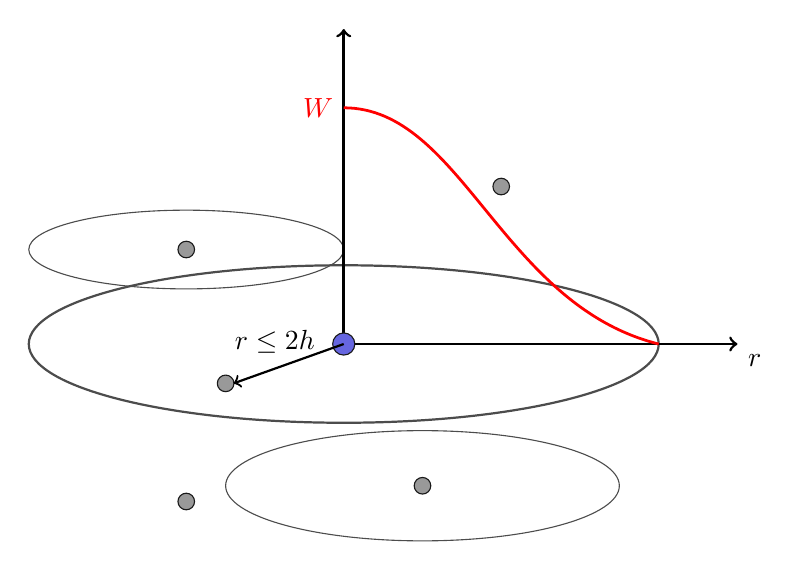
\begin{tikzpicture}
	
	% Others and their ellipse
	\draw [black!90,fill=black!40] (.5,1.5) circle (.3em);
	\draw [black!90,fill=black!40] (0,0) circle (.3em);
	\draw [black!90,fill=black!40] (0,3.2) circle (.3em);
	\draw[black!70] (0,3.2) ellipse (2 and .5);
	\draw [black!90,fill=black!40] (3,.2) circle (.3em);
	\draw[black!70] (3,.2) ellipse (2.5 and .7);
	\draw [black!90,fill=black!40] (4,4) circle (.3em);
	% Ellipses 
	\draw[line width=.8pt,black!70] (2,2) ellipse (4 and 1);
	% Axes
	\draw[->,line width=1pt] (2,2) -- (7,2) node[anchor=north west] {$r$};
	\draw[->,line width=1pt] (2,2) -- (2,6);
	% bezier for kernel 
	\draw[red,line width=1pt]  (6,2) .. controls (4,2.5) and (3.5,5) .. (2,5) node[red,anchor=east] {$W$};
	% main particle, at the end to cover
	\draw [black!90,fill=black!20!blue!60] (2,2) circle (.4em);
	% Arrows 
	\draw[->,line width=.8pt] (2,2) -- (.6,1.5) node[midway, above,xshift=-.5em] {$r\leq2h$};
\end{tikzpicture}
%\includegraphics[scale=.4]{\locpath/figures/flecsph/sph.pdf}
\caption{SPH kernel $W$ and smoothing length $h$ representation}
\label{fig:sph_base}
\end{figure}

The method, as illustrated in figure~\ref{fig:sph_base}, computes the evolution of physical quantities for every particle regarding its neighbors in the radius of its smoothing length $h$. 
The particles in this radius are then valued according to their distance using a smoothing function $W$, also called a kernel. 
The fundamental SPH formulation for any physical quantity $A$ is then to compute with all the neighbors of $b$ of a particle by:
\begin{equation}
A(\vec{r}) \simeq \sum_b \frac{m_b}{\rho_b} A(\vec{r}_b) W ( |\vec{r}-\vec{r}_b|,h)
\end{equation}

On a physics aspect, this method has several advantages:
It can handle deformations, low densities, vacuum, and makes particle tracking easier. 
It also conserves mass, linear and angular momenta, and energy by its construction that implies independence of the numerical resolution. 
Another strong benefit of using SPH is its exact advection of fluid properties. 
Furthermore, the particle structure of SPH easily combines with tree methods for solving Newtonian gravity through N-body simulations.
As a mesh-free method, it avoids the need of grid to calculate the spatial derivatives. 

However, there are cons to consider using SPH: 
It is restricted to low-order rate of convergence on certain PDE formulations; 
It requires careful setup of initial distribution of particles; 
Further, it can be struggle to resolve turbulence-dominated flows and special care must be taken when handling high gradients such as shocks and surface structure of neutron stars.
Many works are leading to handle more cases and to push the limitations of this method \cite{dai2017dual,lind2016incompressible,ren2016dual}.

In this work, we are solving Lagrangian conservation equations (Euler equations) for mass, energy and momentum of an ideal fluid ~\cite{Landau1959}  such that:
\begin{equation}
\frac{d \rho}{d t} = - \rho \nabla \cdot \vec{v}, \quad
\frac{d u}{d t} = \left( \frac{P}{\rho^2} \right) \frac{d \rho}{d t}, \quad
\frac{d \vec{v}}{d t} = - \frac{\nabla P}{\rho}
\end{equation}
with $\rho$ the density, $P$ the pressure, $u$ the internal energy and $v$ the velocity, where $d/dt = \partial_t + \vec{v} \cdot \nabla$ which is convective derivative.

By using the volume element $V_b = m_b / \rho_b$, we can formulate the Newtonian SPH scheme~\cite{rosswog2009} such that
\begin{equation}
\label{eq:rho}
\rho_a = \sum_b m_b W_{ab} (h_a)
\end{equation}
\begin{equation}
\frac{d u_a}{dt} = \frac{P_a}{\rho_a^2} \sum_b m_b \vec{v}_{ab} \cdot \nabla_a W_{ab} 
\end{equation}
\begin{equation}
\frac{d \vec{v}_a}{d t} = - \sum_b m_b \left(\frac{P_a}{\rho_a^2} + \frac{P_b}{\rho_b^2} \right) \nabla_a W_{ab}
\end{equation}
where $W_{ab} = W(| \vec{r}_a - \vec{r}_b |,h)$ is the smoothing kernel. 
The equations we would like to solve allow for emergence of discontinuities from smooth initial data. 
At discontinuities, the entropy increases in shocks. That dissipation occurs inside the shock-front. 
The SPH formulation here is inviscid so we need to handle this dissipation near shocks. 
There are a number of way to handle this problem, but the most widespread approach is to add artificial viscosity (or artificial dissipation) terms in SPH formulation such that:
\begin{equation}
\left(\frac{d u_a}{dt} \right)_{art} = \frac{1}{2} \sum_b m_b \Pi_{ab} \vec{v}_{ab} \cdot \nabla_a W_{ab}
\end{equation}
\begin{equation}
\left(\frac{d\vec{v}_a}{dt} \right)_{art} = - \sum_b m_b \Pi_{ab}\nabla_a W_{ab}
\end{equation}
In general, we can express the equations for internal energy and acceleration with artificial viscosity
\begin{equation}
\label{eq:intern}
\frac{d u_a}{dt} = \sum_b m_b \left(\frac{P_a}{\rho_a^2} + \frac{\Pi_{ab}}{2} \right) \vec{v}_{ab} \cdot \nabla_a W_{ab}
\end{equation}
\begin{equation}
\label{eq:velo}
\frac{d \vec{v}_a}{d t} = - \sum_b m_b \left(\frac{P_a}{\rho_a^2} + \frac{P_b}{\rho_b^2} + \Pi_{ab} \right) \nabla_a W_{ab}
\end{equation}
$\Pi_{ab}$ is the artificial viscosity tensor. 
As long as $\Pi_{ab}$ is symmetric, the conservation of energy, linear and angular momentum is assured by the form of the equation and antisymmetry of the gradient of kernel with respect to the exchange of indices $a$ and $b$. $\Pi_{ab}$ may define different way but here we use~\cite{Monaghan1983} such as: 
\begin{equation}
\Pi_{ab} = \begin{cases}
\frac{- \alpha \bar{c}_{ab} \mu_{ab} + \beta \mu_{ab}^2}{\bar{\rho}_{ab}} & \text{for $\vec{r}_{ab} \cdot \vec{v}_{ab} < 0$} \\
0 & \text{otherwise}
\end{cases}
\end{equation}
\begin{equation}
\mu_{ab} = \frac{\bar{h}_{ab} \vec{r}_{ab} \cdot \vec{v}_{ab}}{r^2_{ab} + \epsilon \bar{h}_{ab}^2}
\end{equation}

Using the usual form $c_s$ as $c_s = \sqrt{\frac{\partial p}{\partial \rho}}$.
The values of $\epsilon$, $\alpha$, and $\beta$ have to be set regarding the problem targeted. 
Here, we use $\epsilon = 0.01h^2$, $\alpha = 1.0$, and $\beta = 2.0$. 

There are many possibilities for the smoothing function, called the kernel. 
As an example the Monaghan's cubic spline kernel is given by:
\begin{equation}
W(\vec{r},h) = \frac{\sigma}{h^D} \begin{cases}
1-\frac{3}{2} q^2 + \frac{3}{4} & \text{if} \indent 0 \leq q \leq 1 \\
\frac{1}{4} (1-q)^3  & \text{if} \indent 1 \leq q \leq 2 \\
0 & \text{otherwise}
\end{cases}
\end{equation}
where $q = r/h$, $r$ the distance between the two particles, $D$ is the number of dimensions and $\sigma$ is a normalization constant with the values:
\begin{equation}
\sigma =  \begin{cases}
\frac{2}{3} & \text{for 1D}  \\
\frac{10}{7 \pi} & \text{for 2D} \\
\frac{1}{\pi} & \text{for 3D}
\end{cases}
\end{equation}

To sum up, the SPH resolution scheme and its routines are presented on algorithm \ref{alg:sph}.
The Equation of State (EOS) and the integration are problem dependent and will be define for each test case in section \ref{sec:applications}. 

\begin{algorithm}
\caption{SPH loop algorithm}\label{alg:sph}
\begin{algorithmic}[1]
\While{not last step}
\State Compute density for each particle (\ref{eq:rho})
\State Compute pressure using EOS 
\State Compute acceleration from pressure forces (\ref{eq:velo})
\State Compute change of internal energy for acceleration (\ref{eq:intern})
\State Advance particles after integration
\EndWhile
\end{algorithmic}
\end{algorithm}

The main downside for the implementation of this method is the requirement for local computation on every particle. 
The particles have to be grouped locally to perform the computation of (\ref{eq:rho}), (\ref{eq:intern}) and (\ref{eq:velo}).
A communication step is needed before and after (\ref{eq:rho}) to get the local physical data to be able to compute (\ref{eq:intern}) and (\ref{eq:velo}).
The tree data structure allows us to perform $O(Nlog(N))$ neighbor search but also add a domain decomposition and distribution layer.

As the SPH method is used in a large panel of fields from astrophysics to fluid mechanic, there are numerous related works. 
We can cite a code developed in the LANL, 2HOT \cite{warren20132hot} that introduced the Hashed Oct Tree structure used in our implementation. 
There is also GADGET-2 \cite{springel2005cosmological}, GIZMO \cite{hopkins2014gizmo} and the most recent publication is GASOLINE \cite{wadsley2017gasoline2} based on PKDGRAV, a specific tree+gravity implementation. 
Several implementations already implement GPU code and tree construction and traversal, one can cite GOTHIC \cite{miki2017gothic}, presenting gravitational tree code accelerated using the latest Fermi, Kepler and Maxwell architectures. But a lot of GPU accelerated work still focused on fluid problems and not on astrophysical problems  \cite{harada2007smoothed,crespo2011gpus}.
We also note that these implementations focus on SPH problems and does not provide a general purpose and multi-physics framework like we intent to provide through FleCSPH and FleCSI. 

\subsection{Gravitation}
For classical problems like fluid flow the gravitation can directly be applied on the particles with the force:
\begin{equation}
	\vec{a_g} = m\vec{g}
\end{equation}

In order to consider astrophysics problems we need to introduice self-gravitation. 
Each particle imply an action on the others base on its distance and mass. 
The equation of gravitation for a particle $i$ with $j$ other particles is: 
\begin{equation}
	\vec{f_a}_i = \sum_j -G \frac{m_i m_j}{|\vec{r_i}-\vec{r_j}|^3} \vec{r_{ij}}
	\label{eq:gravitation}
\end{equation}

This computation involve an $O(N^2)$ complexity and thus is not applicable directly. 
We applied the method called Fast Multipole Method, FMM and discussed in \cite{beatson1997short}.
In this method we compute the gravitation up a approximations. 
The user can refine those approximation changing parameters. 

\begin{figure}
\resizebox {\columnwidth} {!} {
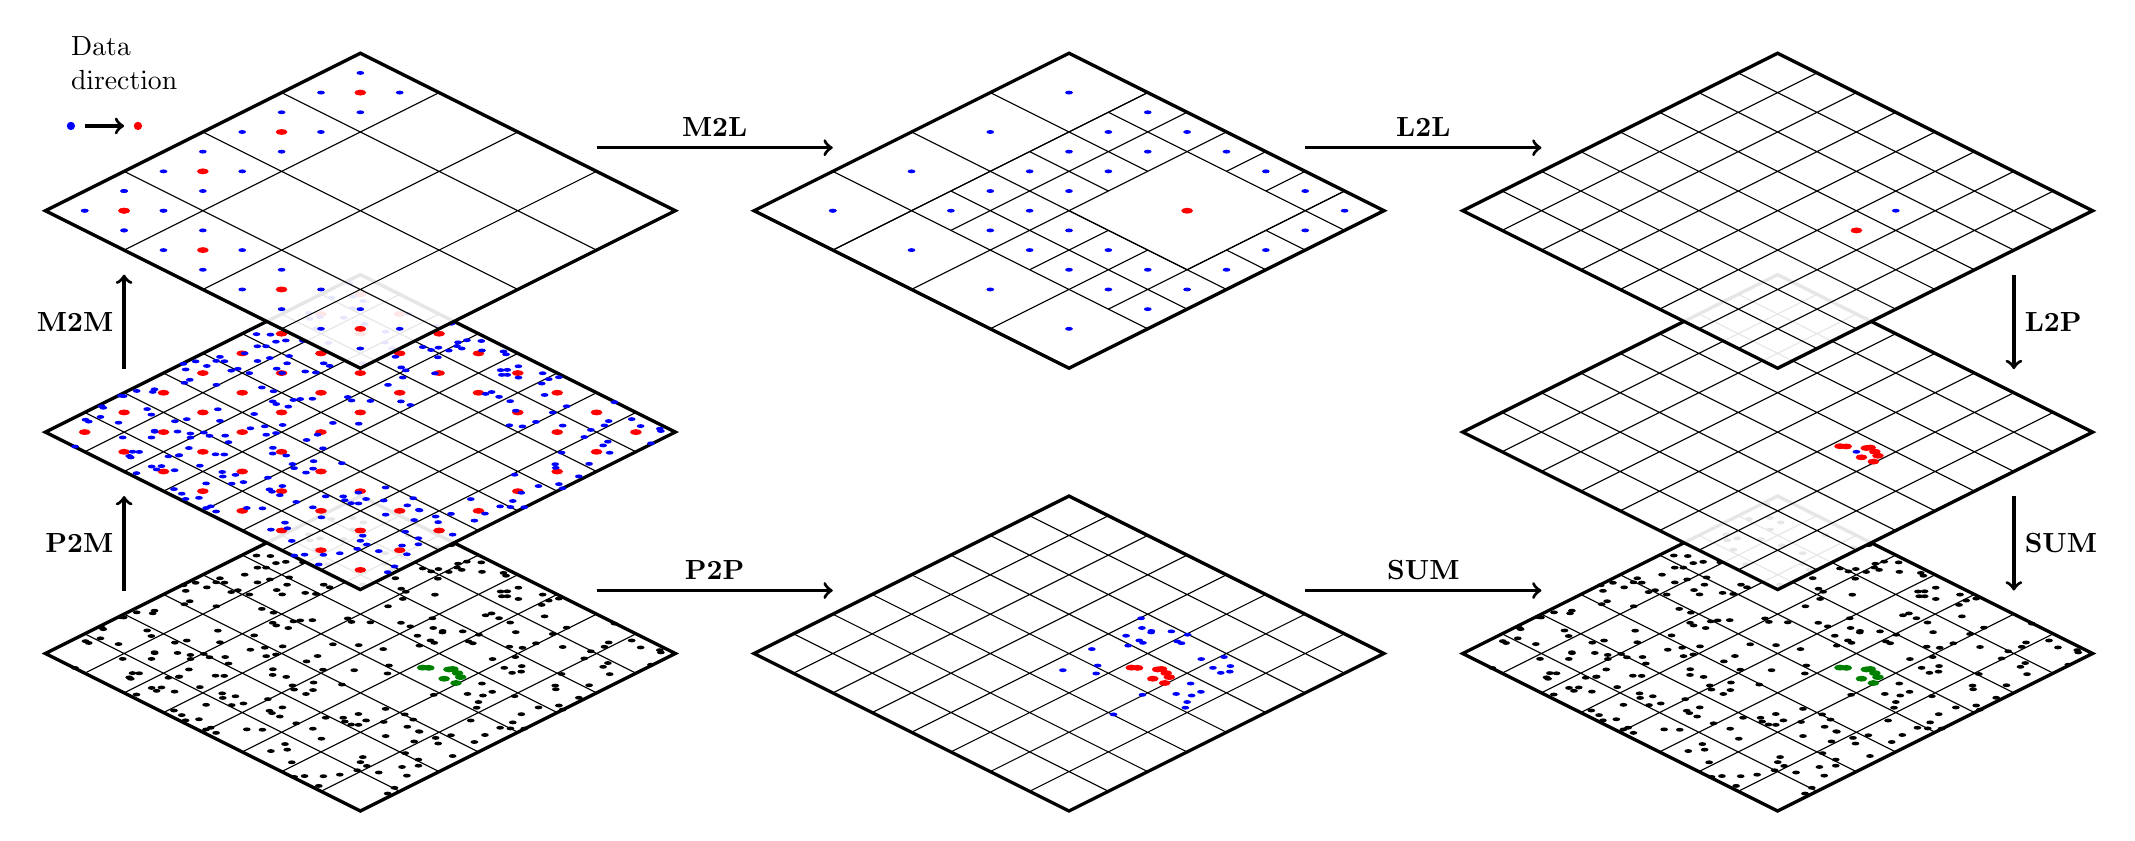
\begin{tikzpicture}
\def\nrand{300}
\def\seed{12}
\def\gridSize{5mm}
\def\gridTotal{4}
% Particles to Multipole
\pgfmathsetseed{\seed}
\begin{scope}[
   		yshift=0,every node/.append style={
    		yslant=0.5,xslant=-1},yslant=0.5,xslant=-1
    ]
    \fill[white,fill opacity=.9] (0,0) rectangle (4,4);
    \draw[black,very thick] (0,0) rectangle (4,4);
	\draw[step=\gridSize, black] (0,0) grid (\gridTotal,\gridTotal);
	\foreach \i in {1,2,...,\nrand}{
    	\pgfmathsetmacro{\x}{(rand)*2+2}
    	\pgfmathsetmacro{\y}{(rand)*2+2}
		% COLOR 
		\ifthenelse{\( \lengthtest{\x cm>2cm} \AND \lengthtest{\x cm<2.5cm} \)}
		{	
			\ifthenelse{ \( \lengthtest{\y cm>1cm} \AND \lengthtest{\y cm<1.5cm} \)}
			{\node at (\x,\y) [black!50!green,circle,fill,inner sep=.7pt,minimum size=3pt]{};}
			{\node at (\x,\y) [circle,fill,inner sep=.7pt]{};}
		}
		{\node at (\x,\y) [circle,fill,inner sep=.7pt]{};}
	}
\end{scope}
\pgfmathsetseed{\seed}
\begin{scope}[
   		yshift=80,every node/.append style={
    		yslant=0.5,xslant=-1},yslant=0.5,xslant=-1
    ]
    \fill[white,fill opacity=.9] (0,0) rectangle (4,4);
    \draw[black,very thick] (0,0) rectangle (4,4);
	\draw[step=5mm, black] (0,0) grid (\gridTotal,\gridTotal);
	\foreach \x in {0,1,...,7}{\foreach \y in {0,1,...,7}{
		\ifthenelse{\( \x<3 \OR \x>5 \)}
		{
			\node at (\x*\gridSize+\gridSize/2,\y*\gridSize+\gridSize/2)[red,circle,fill,inner sep=.7pt,minimum size=3pt]{};
		}
		{	\ifthenelse{ \( \y<1 \OR \y>3 \)}
			{
			\node at (\x*\gridSize+\gridSize/2,\y*\gridSize+\gridSize/2)[red,circle,fill,inner sep=.7pt,minimum size=3pt]{};	
			}{}
		}
	}}
	\foreach \i in {1,2,...,\nrand}{
    	\pgfmathsetmacro{\x}{(rand)*2+2}
    	\pgfmathsetmacro{\y}{(rand)*2+2}
    	\ifthenelse{\( \lengthtest{\x cm<1.5cm} \OR \lengthtest{\x cm>3cm} \)}
		{\node at (\x,\y) [blue,circle,fill,inner sep=.7pt]{};}
		{	\ifthenelse{ \( \lengthtest{\y cm<.5cm} \OR \lengthtest{\y cm>2cm} \)}
			{\node at (\x,\y) [blue,circle,fill,inner sep=.7pt]{};}
			{}
		}
  	}
\end{scope}
\begin{scope}[
   		yshift=160,every node/.append style={
    		yslant=0.5,xslant=-1},yslant=0.5,xslant=-1
    ]
    \fill[white,fill opacity=.9] (0,0) rectangle (4,4);
    \draw[black,very thick] (0,0) rectangle (4,4);
	\draw[step=10mm, black] (0,0) grid (4,4);
	\foreach \x in {0,1}{\foreach \y in {0,...,7}{
		\node at (\x*\gridSize+\gridSize/2,\y*\gridSize+\gridSize/2)[blue,circle,fill,inner sep=.7pt]{};
	}}
	\foreach \x in {0,...,7}{\foreach \y in {6,7}{
		\node at (\x*\gridSize+\gridSize/2,\y*\gridSize+\gridSize/2)[blue,circle,fill,inner sep=.7pt]{};
	}}

	\foreach \x in {0}{\foreach \y in {0,...,3}{				  
		\node at (\x*\gridSize*2+\gridSize,\y*\gridSize*2+\gridSize) [red,circle,fill,inner sep=.7pt,minimum size=3pt]{};
	}}
	\foreach \x in {0,...,3}{\foreach \y in {3}{				  
		\node at (\x*\gridSize*2+\gridSize,\y*\gridSize*2+\gridSize) [red,circle,fill,inner sep=.7pt,minimum size=3pt]{};
	}}
\end{scope}

%PARTICLES TO PARTICLES
\pgfmathsetseed{\seed}
\begin{scope}[
   		yshift=0,xshift=9cm,every node/.append style={
    		yslant=0.5,xslant=-1},yslant=0.5,xslant=-1
    ]
    \fill[white,fill opacity=.9] (0,0) rectangle (4,4);
    \draw[black,very thick] (0,0) rectangle (4,4);
	\draw[step=5mm, black] (0,0) grid (4,4);
	\foreach \i in {1,2,...,\nrand}{
    	\pgfmathsetmacro{\x}{(rand)*2+2}
    	\pgfmathsetmacro{\y}{(rand)*2+2}
    	\ifthenelse{\( \lengthtest{\x cm>1.5cm} \AND \lengthtest{\x cm<3cm} \)}
		{	
			\ifthenelse{ \( \lengthtest{\y cm>.5cm} \AND \lengthtest{\y cm<2cm} \)}
			{
				% COLOR 
				\ifthenelse{\( \lengthtest{\x cm>2cm} \AND \lengthtest{\x cm<2.5cm} \)}
				{	
					\ifthenelse{ \( \lengthtest{\y cm>1cm} \AND \lengthtest{\y cm<1.5cm} \)}
					{\node at (\x,\y) [red,circle,fill,inner sep=.7pt,minimum size=3pt]{};}
					{\node at (\x,\y) [blue,circle,fill,inner sep=.7pt]{};}
				}
				{\node at (\x,\y) [blue,circle,fill,inner sep=.7pt]{};}
			}{}
		}{}
    	%\node at (\x,\y) [circle,fill,inner sep=.7pt]{};
  	}
\end{scope}
%MULTIPOLE TO MULTIPOLE
\begin{scope}[
   		yshift=160,xshift=9cm,every node/.append style={
    		yslant=0.5,xslant=-1},yslant=0.5,xslant=-1
    ]
    \fill[white,fill opacity=.9] (0,0) rectangle (4,4);
    \draw[black,very thick] (0,0) rectangle (4,4);
    \draw[step=10mm, black] (0,3) grid (4,4);
	\draw[step=10mm, black] (0,0) grid (1,3);
	\draw[step=5mm, black] (1,0) grid (2,3);
	\draw[step=5mm, black] (2,2) grid (4,3);
	\draw[step=5mm, black] (2,0) grid (4,.5);
	\draw[step=5mm, black] (3.5,0) grid (4,2);
	% add rectangle
	\draw[black] (2,.5) rectangle (3.5,2);
	% Big part 
	\foreach \x in {0}{\foreach \y in {0,...,3}{				  
		\node at (\x*\gridSize*2+\gridSize,\y*\gridSize*2+\gridSize) [blue,circle,fill,inner sep=.7pt]{};
	}}
	\foreach \x in {0,...,3}{\foreach \y in {3}{				  
		\node at (\x*\gridSize*2+\gridSize,\y*\gridSize*2+\gridSize) [blue,circle,fill,inner sep=.7pt]{};
	}}
	% Smaller one 
	\foreach \x in {2,3}{\foreach \y in {0,...,3}{
		\node at (\x*\gridSize+\gridSize/2,\y*\gridSize+\gridSize/2)[blue,circle,fill,inner sep=.7pt]{};
	}}

	\foreach \x in {2,...,7}{\foreach \y in {4,5}{
		\node at (\x*\gridSize+\gridSize/2,\y*\gridSize+\gridSize/2)[blue,circle,fill,inner sep=.7pt]{};
	}}

	\foreach \x in {7}{\foreach \y in {0,...,3}{
		\node at (\x*\gridSize+\gridSize/2,\y*\gridSize+\gridSize/2)[blue,circle,fill,inner sep=.7pt]{};
	}}
	\foreach \x in {4,5,6}{\foreach \y in {0}{
		\node at (\x*\gridSize+\gridSize/2,\y*\gridSize+\gridSize/2)[blue,circle,fill,inner sep=.7pt]{};
	}}
	\node at (5*\gridSize+\gridSize/2,2*\gridSize+\gridSize/2) [red,circle,fill,inner sep=.7pt,minimum size=3pt]{};
\end{scope}

% Multipole to Particles 
\pgfmathsetseed{\seed}
\begin{scope}[
   		yshift=0,xshift=18cm,every node/.append style={
    		yslant=0.5,xslant=-1},yslant=0.5,xslant=-1
    ]
    \fill[white,fill opacity=.9] (0,0) rectangle (4,4);
    \draw[black,very thick] (0,0) rectangle (4,4);
	\draw[step=5mm, black] (0,0) grid (4,4);
	\foreach \i in {1,2,...,\nrand}{
    	\pgfmathsetmacro{\x}{(rand)*2+2}
    	\pgfmathsetmacro{\y}{(rand)*2+2}
		% COLOR 
		\ifthenelse{\( \lengthtest{\x cm>2cm} \AND \lengthtest{\x cm<2.5cm} \)}
		{	
			\ifthenelse{ \( \lengthtest{\y cm>1cm} \AND \lengthtest{\y cm<1.5cm} \)}
			{\node at (\x,\y) [black!50!green,circle,fill,inner sep=.7pt,minimum size=3pt]{};}
			{\node at (\x,\y) [circle,fill,inner sep=.7pt]{};}
		}
		{\node at (\x,\y) [circle,fill,inner sep=.7pt]{};}
	}
\end{scope}
\pgfmathsetseed{\seed}
\begin{scope}[
   		yshift=80,xshift=18cm,every node/.append style={
    		yslant=0.5,xslant=-1},yslant=0.5,xslant=-1
    ]
    \fill[white,fill opacity=.9] (0,0) rectangle (4,4);
    \draw[black,very thick] (0,0) rectangle (4,4);
	\draw[step=5mm, black] (0,0) grid (4,4);

	\foreach \i in {1,2,...,\nrand}{
    	\pgfmathsetmacro{\x}{(rand)*2+2}
    	\pgfmathsetmacro{\y}{(rand)*2+2}
    	\ifthenelse{\( \lengthtest{\x cm>1.5cm} \AND \lengthtest{\x cm<3cm} \)}
		{	
			\ifthenelse{ \( \lengthtest{\y cm>.5cm} \AND \lengthtest{\y cm<2cm} \)}
			{
				% COLOR 
				\ifthenelse{\( \lengthtest{\x cm>2cm} \AND \lengthtest{\x cm<2.5cm} \)}
				{	
					\ifthenelse{ \( \lengthtest{\y cm>1cm} \AND \lengthtest{\y cm<1.5cm} \)}
					{\node at (\x,\y) [red,circle,fill,inner sep=.7pt,minimum size=3pt]{};}
					{}
				}{}
			}{}
		}{}
	}
	\node at (4*\gridSize+\gridSize/2,2*\gridSize+\gridSize/2) [blue,circle,fill,inner sep=.7pt]{};
\end{scope}
%% MULTIPOLE TO LOCAL
\begin{scope}[
   		yshift=160,xshift=18cm,every node/.append style={
    		yslant=0.5,xslant=-1},yslant=0.5,xslant=-1
    ]
    \fill[white,fill opacity=.9] (0,0) rectangle (4,4);
    \draw[black,very thick] (0,0) rectangle (4,4);
	\draw[step=5mm, black] (0,0) grid (4,4);
	\node at (4*\gridSize+\gridSize/2,2*\gridSize+\gridSize/2) [red,circle,fill,inner sep=.7pt,minimum size=3pt]{};

	\node at (5*\gridSize+\gridSize/2,2*\gridSize+\gridSize/2) [blue,circle,fill,inner sep=.7pt]{};
\end{scope}
% ARROWS AND TEXT
\draw[->,very thick] (-3,2.8) -- (-3,4) node[midway,left] {\textbf{P2M}};
\draw[->,very thick] ([yshift=80]-3,2.8) -- ([yshift=80]-3,4) node[midway,left] {\textbf{M2M}};

\draw[->,very thick] ([yshift=160]3,2.8) -- ([yshift=160]6,2.8) node[midway,above] {\textbf{M2L}};
\draw[->,very thick] ([yshift=160,xshift=9cm]3,2.8) -- ([yshift=160,xshift=9cm]6,2.8) node[midway,above] {\textbf{L2L}};

\draw[<-,very thick] ([yshift=80]21,2.8) -- ([yshift=80]21,4) node[midway,right] {\textbf{L2P}};
\draw[<-,very thick] (21,2.8) -- (21,4) node[midway,right] {\textbf{SUM}};

\draw[->,very thick] (3,2.8) -- (6,2.8) node[midway,above] {\textbf{P2P}};
\draw[->,very thick] ([xshift=9cm]3,2.8) -- ([xshift=9cm]6,2.8) node[midway,above] {\textbf{SUM}};


\draw[->,very thick] (-3.5,8.7cm) node[xshift=-5pt,blue,circle,fill,inner sep=.7pt,minimum size=3pt] (a) {} -- 
 (-3,8.7cm) node[xshift=5pt,red,circle,fill,inner sep=.7pt,minimum size=3pt] (b) {};
\node[align=left] at (-3,9.5cm) {Data\\direction};


\end{tikzpicture}
}
\caption{Fast Multipole Method schematics. Particles to Multipole (P2M), Multipole to Multipole (M2M), Multipole to Particles (M2P), Multipole to Local (M2L), Local to Local (L2L) and Particles to Particles (P2P). Schematic inspired from \cite{yokota2011treecode}}
\end{figure}

This method is based on Taylor series.
The gravitation function of equation~\ref{eq:gravitation} can be approximate on a particle at position $\vec{r}$ by the gravitation computed at the centroid at position $\vec{r_c}$: 
\begin{equation}
 \vec{f}(\vec{r}) = \vec{f}(\vec{r_c}) + ||\frac{\partial\vec{f}}{\partial\vec{r}}||\cdot (\vec{r} - \vec{r_c}) + \frac{1}{2} (\vec{r}-\vec{r_c})^\intercal \cdot   ||\frac{\partial\vec{f}}{\partial\vec{r} \partial\vec{r}}|| \cdot (\vec{r} - \vec{r_c})
 \end{equation}

 From equation~\ref{eq:gravitation} we compute the term $||\frac{\partial\vec{f}}{\partial\vec{r}}||$:s
 \begin{equation}
\frac{\partial\vec{f}}{\partial\vec{r}} =
- \sum_p \frac{m_p}{|\vec{r_c}-\vec{r_p}|^3}
\begin{bmatrix}
1 - \frac{3(x_c-x_p)(x_c-x_p)}{|\overline{r_c}-\overline{r_p}|^2} & -\frac{3(y_c-y_p)(x_c-x_p)}{|\overline{r_c}-\overline{r_p}|^2}  & -\frac{3(z_c-z_p)(x_c-x_p)}{|\vec{r_c}-\vec{r_p}|^2}  \\
-\frac{3(x_c-x_p)(y_c-y_p)}{|\vec{r_c}-\vec{r_p}|^2}  & 1 - \frac{3(y_c-y_p)(y_c-y_p)}{|\vec{r_c}-\vec{r_p}|^2} &  -\frac{3(z_c-z_p)(y_c-y_p)}{|\vec{r_c}-\vec{r_p}|^2}\\
- \frac{3(x_c-x_p)(z_c-z_p)}{|\vec{r_c}-\vec{r_p}|^2}   &  -\frac{3(y_c-y_p)(z_c-z_p)}{|\vec{r_c}-\vec{r_p}|^2} &  1- \frac{3(z_c-z_p)(z_c-z_p)}{|\vec{r_c}-\vec{r_p}|^2} \\
\end{bmatrix}
 \end{equation}

And we propose a compact version of the matrix with: 
 
\begin{equation}
 ||\frac{\partial f^a}{\partial r^b}|| = -\sum_c \frac{m_c}{|\vec{r}-\vec{r_c}|^3} \Big[ \delta_{ab} - \frac{3.(r^a-r_c^a)(r^b-r_c^b)}{|\vec{r}-\vec{r_c}|^2} \Big] 
\end{equation}

With $\delta_{ab}$ the Kronecker delta:
\begin{equation}
\delta_{ab} = 
\begin{cases}
    1, & \text{if $a = b$}.\\
    0, & \text{if $a\neq b$}.
  \end{cases}
\end{equation}

We note that $a$ and $b$ variate from 0 to 2 and $r^0=x$, $r^1=y$, and $r^2=z$ as usual sense. 

For the term $||\frac{\partial\vec{f}}{\partial\vec{r} \partial\vec{r}}||$ we give the compact version by:
\begin{equation}
\begin{aligned}
||\frac{\partial^2 f^a}{\partial r^b \partial r^c}|| = - \sum_c \frac{3 m_c}{|\vec{r}-\vec{r_c}|^5} \Big[ & \frac{5(r^a-r_c^a)(r^b-r_c^b)(r^c-r_c^c)}{|\vec{r}-\vec{r_c}|^2} - \\ 
		 & \left( \delta_{ab} (r^c-r_c^c)+\delta_{bc} (r^a-r_c^a)+\delta_{ac} (r^b-r_c^b) \right) \Big] 
\end{aligned}
\end{equation} 

 \begin{figure}
 \end{figure}

The method is summed up in figure with the different equations.
We consider Centers Of Mass, COM, to be the centroid of particles based on their position. 
In several steps the information is first transmitted to the COMs, computing their position and mass. 


\section{Applications of SPH} 
The previous equations are generic and describe the behavior of SPH method. 
In order to check our 

\subsection{Sod shock tube}
The Sod shock tube is the test consisting of a one-dimensional Riemann problem with the following initial parameters~\cite{sod1978}.
\begin{equation}
(\rho, v, p)_{t=0} = \begin{cases}
(1.0,0.0,1.0) & \text{if} \indent 0 < x \leq 0.5 \\
(0.125,0.0,0.1) & \text{if} \indent 0.5 < x < 1.0
\end{cases}
\end{equation}
In our code, we use the same initial data as in section \ref{sec:intro_sph} with ideal gas EOS such as:
\begin{equation}
P(\rho,u) = (\Gamma - 1) \rho u
\end{equation}
where $\Gamma$ is the adiabatic index of the gas, we set $\Gamma = 5/3$. 

\begin{figure}[t!]
\centering
\includegraphics[width=\columnwidth]{\locpath/figures/sph/{sodtube_width}.png}
\caption{Sod shock tube with FleCSPH}
\label{fig:sodtube}
\end{figure}

This test is used to check the physical accuracy of the code and thus the tree search itself.
A simulation of our Sod shock experimentation is presented on Fig.~\ref{fig:sodtube} and shows physically correct results. 

\subsection{Sedov blast wave}
A blast wave is the pressure and flow resulting from the deposition of a large amount of energy in a small very localized volume. 
There are different versions of blast wave test and we consider comparing it with the analytic solution for a point explosion as given by Sedov~\cite{sedov1946}, making the assumption that the atmospheric pressure relative to the pressure insider the explosion negligible. 
Here, we test 2D blast wave. In this simulation, we use ideal gas EOS with $\Gamma = 5/3$ and we are assuming that the undistributed area is at rest with a pressure $P_0 = 1.0 \time 10^{-5}$. The density is constant $\rho_0$, also in the pressurized region. 

\begin{figure}[t]
\centering
\includegraphics[width=\columnwidth]{\locpath/figures/sph/{sedov_flecsph_results}}
\caption{Sedov Blast Wave with FleCSPH at respectively $t=0.01$, $t=0.03$, $t=0.06$ and $t=0.1$}
\label{fig:sedov}
\end{figure}

An example of our Sedov Blast wave experimentation is presented on Fig.~\ref{fig:sedov} and shows physically correct results.

\subsection{Fluid flow}
After performing the tests regarding the physics reliability, we worked on fluid flow problem in 2D and 3D to reach high number of particles. 
The details can be found in \cite{gomez2012sphysics}.
This test is based on an ideal EOS given by:
\begin{equation}
P = B \Big[ \big( \frac{\rho}{\rho_0} \Big)^\gamma -1 \Big] 
\end{equation}
with $\gamma = 7$ and $B = c_0\rho_0/\gamma$ being $\rho_0 = 1000 \, kg.m^{-3}$ the reference density.

\begin{figure}[t!]
\centering
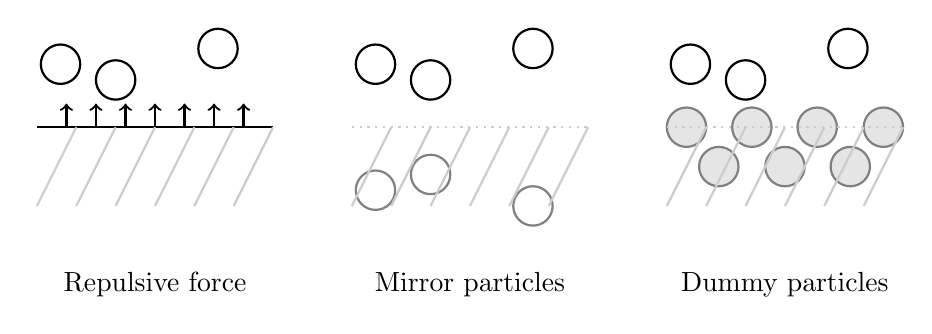
\begin{tikzpicture}[thick]
% Mathematical reflection
\draw (0.3,.8) circle (.25cm) node[pos=.5] (p0) {};
\draw (1,.6) circle (.25cm) node[pos=.5] (p1) {};
\draw (2.3,1) circle (.25cm) node[pos=.5] (p2) {};
\draw (0,0) -- (3,0);
\foreach \i in {1,...,6}{
	\draw[black!20] (.5*\i-.5,-1) -- (.5*\i,0);
}
% Forces
\foreach \i in {1,...,7}{
	\draw[->] (.375*\i,0) -- (.375*\i,.3);
}
\node at (1.5,-2) {Repulsive force};

% Mirror 
\draw (4.3,.8) circle (.25cm) node[pos=.5] (p0) {};
\draw (5,.6) circle (.25cm) node[pos=.5] (p1) {};
\draw (6.3,1) circle (.25cm) node[pos=.5] (p2) {};
\draw[black!50] (4.3,-.8) circle (.25cm) node[pos=.5] (mii1) {};
\draw[black!50] (5,-.6) circle (.25cm) node[pos=.5] (mii2) {};
\draw[black!50] (6.3,-1) circle (.25cm) node[pos=.5] (mii3) {};
\draw[black!20,dotted] (4,0) -- (7,0);
\foreach \i in {1,...,6}{
	\draw[black!20] (.5*\i-.5+4,-1) -- (.5*\i+4,0);
}
\node at (5.5,-2) {Mirror particles};

% Dummies
\draw[black!50,fill=black!10] (8.25,0) circle (.25cm) node[pos=.5] (d0) {};
\draw[black!50,fill=black!10] (9.08,0) circle (.25cm) node[pos=.5] (d1) {};
\draw[black!50,fill=black!10] (9.91,0) circle (.25cm) node[pos=.5] (d2) {};
\draw[black!50,fill=black!10] (10.75,0) circle (.25cm) node[pos=.5] (d3) {};
% second layer
\draw[black!50,fill=black!10] (8.66,-.5) circle (.25cm) node[pos=.5] (d4) {};
\draw[black!50,fill=black!10] (9.50,-.5) circle (.25cm) node[pos=.5] (d5) {};
\draw[black!50,fill=black!10] (10.33,-.5) circle (.25cm) node[pos=.5] (d6) {};
%\draw (1,-.25) circle (.25cm) node[pos=.5] (d4) {};
%normal parts
\draw (8.3,.8) circle (.25cm) node[pos=.5] (p0) {};
\draw (9,.6) circle (.25cm) node[pos=.5] (p1) {};
\draw (10.3,1) circle (.25cm) node[pos=.5] (p2) {};
\draw[dotted,black!20] (8,0) -- (11,0);
\foreach \i in {1,...,6}{
	\draw[black!20] (.5*\i-.5+8,-1) -- (.5*\i+8,0);
}
\node at (9.5,-2) {Dummy particles};
\end{tikzpicture}
\caption{Different boundaries condition methods}
\label{fig:SPH:boundaries}
\end{figure}

For this experiment, realistic boundaries conditions were needed. 
Several methods are possible with SPH we focused on the main ones, the repulsive wall, the mirror particles \cite{libersky1991smooth} and the dummies particles implementation \cite{adami2012generalized}. 
Those boundaries conditions implementation are presented in figure~\ref{fig:SPH:boundaries}.

For the current implementation, we used the dummies particles method.
The wall particles are just considered as normal particles, with specific equations, and their quantities are evolved during the run. 
The main difference is that their position does not evolve at the end of the step.
They are identified in the code with a specific type, provided during the data generation. 

\subsection{Astrophysics: neutron stars coalescence}

The final aim of our tests is to simulate astrophysical events. 
We are interested in one of the most important event recently discovered. 
Last year the Laser Interferometer Gravitational Wave, LIGO, detected the first gravitational wave generated by binary neutron stars merging \cite{abbott2017gw170817} and also more complexes event with Binary Black Holes coalescence in \cite{abbott2017gw170814}.


\subsubsection{Solving Lane-Emden Equation}

We need to determine the density function based on the radius. 

As we consider the star as a polytropic fluid, we use the equation of Lane-Emden which is a form of the Poisson equation: 

\begin{equation}\label{eq_LaneEmden}
  \frac{d^2\theta}{d \xi^2}+ \frac{2}{\xi}\frac{d\theta}{d\xi}+\theta^n = 0
\end{equation}

With $\xi$ and $\theta$ two dimensionless variables. 
There is only exact solutions for a polytropic index $n = 0.5$, $1$ and $2$.
In our work we use a polytropic index of $1$ which can correspond to a NS simulation.

For $n=1$ the solution of equation \ref{eq_LaneEmden} is: 

\begin{equation}
\theta(\xi)=\frac{sin(\xi)}{\xi}
\end{equation}

We note $\xi_1 = \pi$, the first value of $\xi$ as $\theta(\xi) = 0$.
$\theta(\xi)$ is also defined as: 
\begin{equation}
 \theta(\xi) = \Big(\frac{\rho(\xi)}{\rho_c}\Big)^{\frac{1}{n}}  = \frac{\rho(\xi)}{\rho_c}
\end{equation}

With $\rho_c$ the internal density of the star and $\rho$ the density at a determined radius. $\xi$ is defined as:  
$$ \xi = Ar = \sqrt{\frac{4\pi G}{K(n+1)}\rho_c^{(n-1)/n}} \times r = \sqrt{\frac{2\pi G}{K}}\times r \mbox{ (for } n=1 \mbox{)}$$

With $K$ a proportionality constant.

From the previous equations we can write the stellar radius $R$ as:
\begin{equation}
R = \sqrt{\frac{K(n+1)}{4\pi G}}\rho_c^{(1-n)/2}\xi_1 = \sqrt{ \frac{K}{2\pi G} } \times \xi_1
\end{equation} 

(We note that for $n=1$ the radius does not depend of the central density.)

If, for example, we use dimensionless units as $G=R=M=1$ (for the other results we use CGS with $G = 6.674 \times 10^{-8} cm^3g^{-1}s^{-2}$) 
We can compute K as: 
\begin{equation}
\label{eq:constant}
K = \frac{R^2  2 \pi G}{\xi_1^2}
\end{equation}

\begin{center}
\begin{tabular}{c|c|c|c|c|}
 & $NS_1$ & $NS_2$ & $NS_3$ & $NS_4$ \\ 
\hline 
Radius (cm) & $R=G=M=1$ & 1500000 & 1400000 & 960000 \\ 
\hline 
K & 0.636619 & 95598.00 & 83576.48 & 39156.94\\ 
\hline 
\end{tabular}
\end{center} 

Then we deduce the density function of $r$ as :

$$\rho(\xi) = \frac{sin(A\times r)}{A \times r} \times \rho_c \mbox{ with } A = \sqrt{\frac{2\pi G}{K}}
$$

As we know the total Mass $M$, the radius $R$ and the gravitational constant $G$ we can compute the central density as: 

$$ \rho_c = \frac{M A^3}{4 \pi (sin(AR)-ARcos(AR)) } $$

Then we normalize the results to fit $R = M = G = 1$: $K' = K/(R^2G) $, $m_i' = m_i/M $, $h_i' = h_i / R$, $\vec{x_i}' = \vec{x_i}/R$ 

\section{Conclusion}



%%%%%%%%%%%%%%%%%%%%%%%%%%%%%%%%%%%%%%%%%%%%%%%%%%%%%%%%%%%%%%%%%%%%%
%                                                                   %
%	CHAPTER TWO, FLECSPH.                                           %
%                                                                   %
%%%%%%%%%%%%%%%%%%%%%%%%%%%%%%%%%%%%%%%%%%%%%%%%%%%%%%%%%%%%%%%%%%%%%
%%%%%%%%%%%%%%%%%%%%%%%%%%%%%%%%%%%%%%%%%%%%%%%%%%%%%%%%%%%%%%%%%%%%%
%                                                                   %
%	CHAPTER TWO, HARDWARE IN HPC                                    %
%                                                                   %
%%%%%%%%%%%%%%%%%%%%%%%%%%%%%%%%%%%%%%%%%%%%%%%%%%%%%%%%%%%%%%%%%%%%%

\chapter{Hardware in HPC}

\section{Introduction}

Parallel models address most of the key points for application performance, but it may also depend on architectures hardware, which may influence how to consider the problems' resolution. 
Thus, the knowledge of hardware architecture is essential to reach performances through optimizations.
Even if the current software, API, framework or runtime already handle most of the optimizations, the last percents of performance gain are architecture dependent. 
In this chapter, we describe the most important devices architectures from classical processors, General Purpose Graphics Processing Units (GPGPUs), Field Programmable Gate Arrays (FPGAs) and Application-Specific Integrated Circuits (ASICs).
This study focuses on multi-core processors and GPUs as we based our tests on these devices. 

This chapter describes the architecture of some remarkable supercomputers. 
This comes with the description of interconnection network for the most used interconnection topologies. 

We choose to present the architectures in a chronological order following the models presented in the previous chapter - SISD, MIMD and SIMD/SIMT - and presenting the most recently released technologies.
We also present the optimizations of current technologies with the rise of parallelism and new types of memories.

\section{Early improvements of Von Neumann machine}
In this section, we present the different hardware evolution from the 1970s single core processors to modern multi-core and many-core architectures that are the milestones, and the basic units, for building supercomputers. 
We can observe the most important optimizations that are always implemented in the most recent machines: in/out of order processors, pre-fetching strategies, vectorization and the memory technologies breakthroughs. 

\subsection{Single core processors}
The first processors were developed in the 1970s and were built using a single computation core as described in the Von Neumann model. 
The single core processors were improved with many optimizations from the memory, the order of the instructions and the frequency to increase.

\subsubsection{Transistor shrink and frequency}
\index{Frequency}
Many new approaches to produce smaller transistors have been discovered.
Transistor sizes were about 10$\mu m$ in 1971 and reach 10$nm$ in current machines.
This allowed the constructors to add more transistors on the same die and build more complex ISA and features for the CPUs. 

In parallel of the shrink of transistors, the main feature for better performances with the single core architectures came from the frequency augmentation, the clock rate. 
As the clock rate increases, more operations can be performed on the core in the same amount of time. 
In the 1970s, the frequency was about 4 MHz allowing a maximum of 4 million of cycles per seconds. 
Nowadays, single cores can work at a frequency of 4GHz and even 5GHz performing billions of operations per cycles, but the following sections will demonstrate that due to power consumption and coding considerations, frequency is no longer used to improve performances. 

\subsubsection{In/Out-Of-Order execution} 
\index{In/Out of Order}
In-order-process is described in the previous chapter. 
This control unit fetches instructions and the operands from memory. 
The ALU then computes the operation before the final result is stored to the memory.

In this model, the time to perform an instruction is the accumulation of: instruction fetching + operand(s) fetching + \textit{computation} + result storage.
This time may be high regarding the use of the ALU for \textit{computation}, technically just one clock cycle. 
The idea of \textit{out-of-order} execution is to compute the instructions without following the Program Counter order. 
Indeed, for independent tasks, (indicated by dependency graphs) while the process fetches the next instruction data, the ALU can perform another operation with already available operands.
This leads to better usage of computational resources in the CPU, and thus better overall performances. 

\subsubsection{Vectorization} 
\index{Vectorization}
\index{Unrolling}
\index{Loop tiling}
Vector processors allow the instructions to be executed at the same time in a SIMD manner. 
If the same instruction is executed on coalescent data they can be executed in the same clock cycle. 
For an example, we can execute operations simultaneously on four to eight floats with a bus size of 128 or 256 bits.
This requires specific care for coding with \textit{unrolling} and \textit{loop tiling} to avoid bad behavior leading to poor performances and will be addressed later in this study.
The latest architectures vectorization imposes to slightly lower the frequency of processors. 

\index{Cray-1}
The Cray-1 supercomputer\cite{russell1978cray}, installed in 1975 in the Los Alamos National Laboratory, is a perfect example of vector processor supercomputer.
This supercomputer was designed by Seymour Cray, the founder of Cray Research, and was able to deliver up to 160 MFLOPS based on vector processor.
It was the fastest supercomputer in 1978 and due to its shape and price it was humorously called \textit{the world's most expansive love-seat}. 

\begin{figure}[t!]
\begin{center}
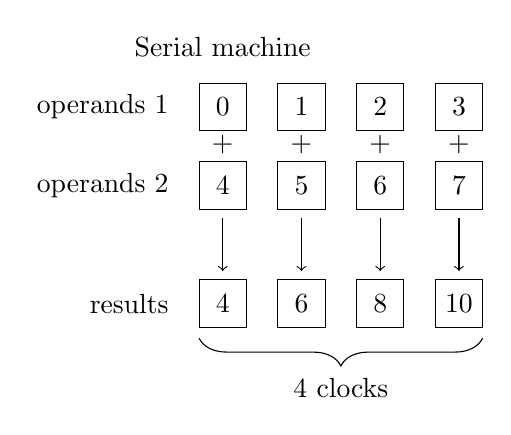
\begin{tikzpicture}
\foreach \x in {0,...,3}
{
	% Draw the rectangle 
	\draw (\x,0) rectangle (\x+.6,.6) node[pos=.5] (res\x) {
		\pgfmathparse{4+\x*2}
		\pgfmathprintnumber[precision=0]
        \pgfmathresult
    };
	\draw (\x,1.5) rectangle (\x+.6,2.1) node[pos=.5] (op2\x)  {
		\pgfmathparse{\x+4}
		\pgfmathprintnumber[precision=0]
        \pgfmathresult
    };
	\draw (\x,2.5) rectangle (\x+.6,3.1) node[pos=.5] (op1\x) {\x};
	% Draw the arrows for result
	\draw[->] ([yshift=-5pt]op2\x.south) -- ([yshift=5pt]res\x.north);
	\node at ([yshift=-7pt]op1\x.south) {$+$};
}
% add the arrow on top for clocks 
\draw [decorate,decoration={brace,amplitude=10pt,mirror,raise=4pt},yshift=0pt]
(0.,0) -- (3.6,0) node [black,midway,below,yshift=-15pt] {4 clocks};

\node[anchor=east] at ([xshift=-10pt]res0.west) {results};
\node[anchor=east] at ([xshift=-10pt]op10.west) {operands 1};
\node[anchor=east] at ([xshift=-10pt]op20.west) {operands 2};

\node[thick] at ([yshift=15pt]op10.north) {Serial machine};


% Add the name of architecture, classical serial 

% Add line name 
\end{tikzpicture}
\hspace{1cm}
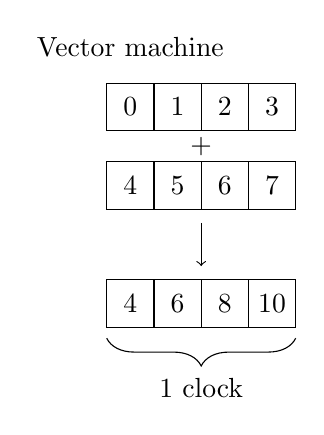
\begin{tikzpicture}
\foreach \x in {0,...,3}
{
	% Draw the rectangle 
	\draw (\x*.6,0) rectangle (\x*.6+.6,.6) node[pos=.5] (res\x) {
		\pgfmathparse{4+\x*2}
		\pgfmathprintnumber[precision=0]
        \pgfmathresult
    };
	\draw (\x*.6,1.5) rectangle (\x*.6+.6,2.1) node[pos=.5] (op2\x)  {
		\pgfmathparse{\x+4}
		\pgfmathprintnumber[precision=0]
        \pgfmathresult
    };
	\draw (\x*.6,2.5) rectangle (\x*.6+.6,3.1) node[pos=.5] (op1\x) {\x};
	% Draw the arrows for result
}

% Just onw arrow and plus sign 
\draw[->] ([yshift=-5pt]1.2,1.5) -- ([yshift=5pt]1.2,.6);
\node at ([yshift=-6pt]1.2,2.5) {$+$};

\draw [decorate,decoration={brace,amplitude=10pt,mirror,raise=4pt},yshift=0pt]
(0.,0) -- (2.4,0) node [black,midway,below,yshift=-15pt] {1 clock};

\node[thick] at ([yshift=15pt,]op10.north) {Vector machine};
\end{tikzpicture}
\end{center}
\caption{Vectorized processeur example on 4 integer addition: 128 bits wide bus}
\label{fig:2_HARD:vector}
\end{figure}

The behavior of vector machine is presented on figure~\ref{fig:2_HARD:vector} for a 16 bytes vector machine (4 integer of 4 bytes = 128 bits bus). 
We see on the left that performing the 4 operations requests in 4 cycle and, at the opposite, 1 cycle on the right with the vectorized machine.\\

Linked with the CPU optimizations, the memory optimizations also needs to be considered. 
Even if the ALU can perform billions of operations per second, it needs to be fed with data by fast transfers.

\subsubsection{Memory technology evolution}

The memories technologies optimizations address several aspects. 
The early 1980s saw the augmentation of bus size from 4 bits to presently 32 bits for single precision and 64 bits for double precision. 
Buses with 128 bits or 256 bits can also be used to allow vectorization presented just before. 

Different kind of technologies are considered in this study: the SRAM and DRAM. 

\paragraph{SRAM: }
\index{Static Random Access Memory}
The Static Random Access Memory (SRAM) is built using so called "flip-flop" circuits that can store data at any time time with no time lost in "refresh operations".
This kind of memory is very expensive to produce due to the number of transistors by memory cell, therefore, it is usually limited for small amounts of storage. 
The SRAM is mainly used for cache memory. 

\paragraph{DRAM: }
\index{Dynamic Random Access Memory}
The Dynamic Random Access Memory (DRAM) is based on transistors and capacitors to store binary information.
This memory is less expensive to produce but needs to be refreshed at a determined frequency, otherwise the data are lost. 
This refresh step is a read-write operation on the whole memory at a specific frequency. 
There are several sub-categories of DRAM used in different device depending on the way the bus are used with Single Data Rate (SDR), Double Data Rate (DDR) and Quad Data Rates (QDR). 
The number of data carried can vary from one times to four times, but the limitation of those products is the price and are constantly rising. 

The latest more efficient memory is the 3D memory.
This is a stack of the different components instead of usual 2D distribution.
This memory, 3D XPoint, was created by Intel and Micron Technology and announced in July 2015. 
It can now be find in the NVIDIA GPUs, named 3D-stacked in P100 and V100.

\subsubsection{Cache memory: }
\index{Cache mechanism}
\begin{figure}[t!]
\centering
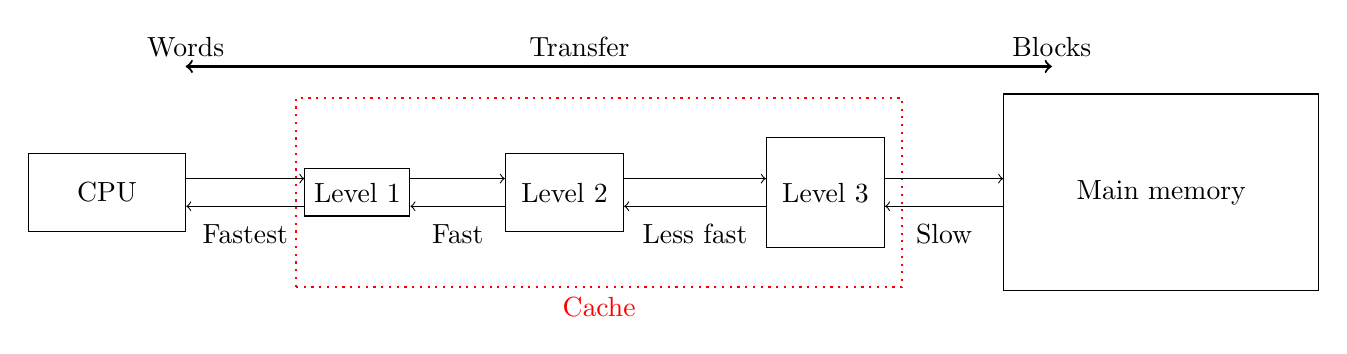
\begin{tikzpicture}
\node (rect) at (0,0) [draw,minimum width=2cm,minimum height=1cm] (cpu) {CPU};
\node[right = 1.5cm of cpu] (rect) [draw,minimum width=1cm,minimum height=.6cm] (cache_1) {Level 1};
\node[right = 1.2cm of cache_1] (rect) [draw,minimum width=1.5cm,minimum height=1cm] (cache_2) {Level 2};
\node[right = 1.8cm of cache_2] (rect) [draw,minimum width=1.5cm,minimum height=1.4cm] (cache_3) {Level 3};
\node[right = 1.5cm of cache_3] (rect) [draw,minimum width=4cm,minimum height=2.5cm] (ram) {Main memory};

\draw[thick,draw,red,dotted] (2.4,-1.2) rectangle  (10.1,1.2);
\node[below,red,thick] at (6.25,-1.2) {Cache}; 
% links 
\draw[->] ([yshift=5pt]cpu.east) -- ([yshift=5pt]cache_1.west);
\draw[<-] ([yshift=-5pt]cpu.east) -- ([yshift=-5pt]cache_1.west) node[midway,yshift=-10pt] {Fastest};

\draw[->] ([yshift=5pt]cache_1.east) -- ([yshift=5pt]cache_2.west);
\draw[<-] ([yshift=-5pt]cache_1.east) -- ([yshift=-5pt]cache_2.west) node[midway,yshift=-10pt] {Fast};

\draw[->] ([yshift=5pt]cache_2.east) -- ([yshift=5pt]cache_3.west);
\draw[<-] ([yshift=-5pt]cache_2.east) -- ([yshift=-5pt]cache_3.west) node[midway,yshift=-10pt] {Less fast};

\draw[->] ([yshift=5pt]cache_3.east) -- ([yshift=5pt]ram.west);
\draw[<-] ([yshift=-5pt]cache_3.east) -- ([yshift=-5pt]ram.west) node[midway,yshift=-10pt] {Slow};

\draw[<->,thick] (1,1.6) node[above]{Words} -- (12,1.6) node[above] {Blocks};
\node[above] at (6,1.6) {Transfer}; 
\end{tikzpicture}
\caption{Cache memory technology on three levels L1, L2 and L3}
\label{fig:2_HARD:caches}
\end{figure}
Cache is a memory mechanism that is useful to consider when targeting performance. 
The main idea of cache technology is presented on figure~\ref{fig:2_HARD:caches}.
This memory is built hierarchically over several levels. 
L1 is the closest to the CPU followed by L2 with generally no levels past L3 except on specific architectures. 
When looking for data, the CPU first checks if the data is present in the L1 cache, otherwise it will look in L2 and L3 to get the data to higher level. 
From the main memory to the L3 cache \textit{blocks} are exchanged, by chunks. 
With levels L1 and L2, lines of information are exchanged, usually referred to as \textit{words}.
This is based on the idea that if a data is used, it shall be used again in the near future.
Many cache architectures exist: direct, associative, fully associative, etc. 
Cache-hits occur when the data required is present in cache versus a cache-miss occurs when it has to be retrieved from lower levels or main memory. 
The ratio of cache-miss has to be kept low in a program in order to reach performance, and the impact may be very high.

\subsubsection{Pre-fetching} 
\index{Pre-fetching}
Pre-fecthing was developed based on memory optimization and especially for the cache.
When data are not available in L1 cache, it has to be moved from either L2 to L1 or L3 to L2 to L1 or in the worst case from RAM to L3 to L2 to L1. 
Pre-fecthing technology is a way to, knowing the next instructions operands, pre-fetch the data in closer cache before the instruction is decoded. 
The pre-fetch can either be hardware or software implemented and can concern data and even instructions.

\subsection{Multi-CPU servers and multi-core processors}
Around the beginning of the 2000s, the limitations of single core processors were very important. 
The frequency was already high and requested more power consumption causing more heat dissipation. 
The first solution to this problem was to provide multi-CPU devices, embedding several CPU on the same motherboard and allowing them to share memory. 
The evolution of the mono-core is the multi-core having several processing units on the same die allowed more optimization inside the die and combining all the advantages of single core processors.
But by embedding each CPU, the function and units required consume $n$ times more energy with cumulate heat effects.
Thus, unable to answer the constant augmentation of computational power needed for research and HPC, IBM was the first company to create a multi-core CPU in 2001, the Power4. 

Compared to the core inside multi-CPU, multi-core CPU shared one of the material (L3 caches, buses, etc.) and are implemented on the same due; this allows to reach the same CPU performances with less transistors and less power consumption, avoiding most of the heating issues. 

\begin{figure}
\centering 
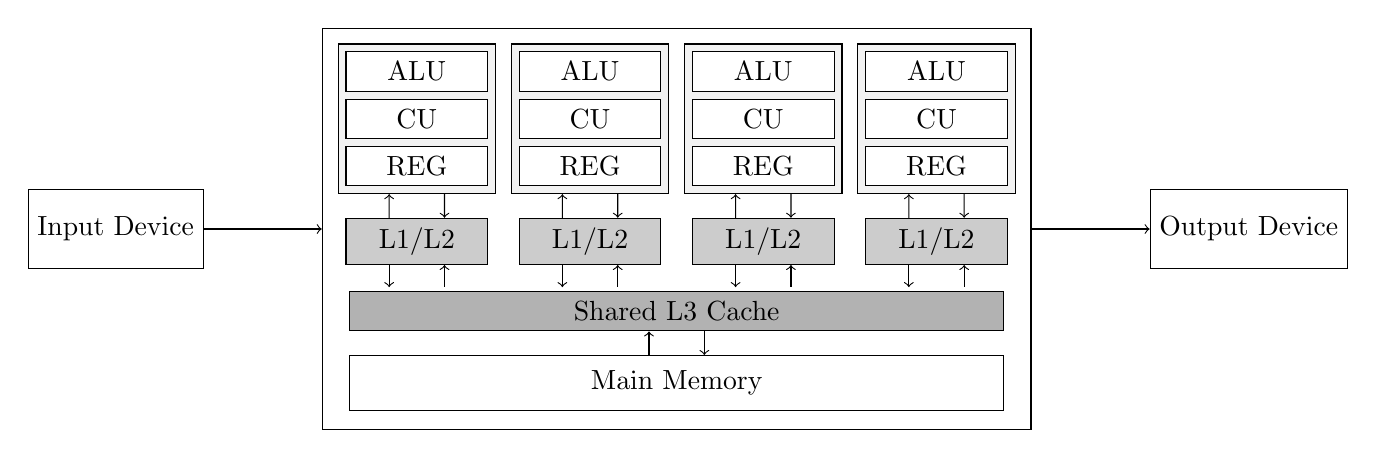
\begin{tikzpicture}

\node (rect) at (0,0) [draw,minimum width=2cm,minimum height=1cm] (input) {Input Device};

\node[right = 1.5cm of input] (rect) [draw,minimum width=9cm,minimum height=5.1cm] (machine) {};

\node[fill=black!30] (rect) at ([yshift=-3.6cm]machine.north) [draw,minimum width=8.3cm,minimum height=.5cm] (l3) {Shared L3 Cache};

\foreach \x in {0,...,3}{
	\node[anchor=north west,fill=black!5] (rect) at ([yshift=-.2cm,xshift=\x*2.2cm+.2cm]machine.north west) [draw,minimum width=2cm,minimum height=1.9cm] (cpu\x) {};

	\node[anchor=north west,fill=white] (rect) at ([yshift=-.1cm,xshift=.1cm]cpu\x.north west) [draw,minimum width=1.8cm,minimum height=.5cm] {ALU};
	\node[anchor=north west,fill=white] (rect) at ([yshift=-.7cm,xshift=.1cm]cpu\x.north west) [draw,minimum width=1.8cm,minimum height=.5cm] {CU};
	\node[anchor=north west,fill=white] (rect) at ([yshift=-1.3cm,xshift=.1cm]cpu\x.north west) [draw,minimum width=1.8cm,minimum height=.5cm] {REG};
	% Cache memory
	\node[anchor=north west,fill=black!20] (rect) at ([yshift=-.3cm,xshift=.1cm]cpu\x.south west) [draw,minimum width=1.8cm,minimum height=.5cm] (l1\x) {L1/L2};
	% Arriw 
	\draw[->] ([xshift=-10pt]l1\x.north) -- ([xshift=-10pt]cpu\x.south);
	\draw[<-] ([xshift=10pt]l1\x.north) -- ([xshift=10pt]cpu\x.south);
	% Arrow to L3
	\draw[->] ([xshift=-10pt]l1\x.south) -- ([xshift=-10pt,yshift=-8pt]l1\x.south);
	\draw[<-] ([xshift=10pt]l1\x.south) -- ([xshift=10pt,yshift=-8pt]l1\x.south);

	%\draw[<-] ([xshift=10pt]l1\x.south) |- (l3.north);
	
}


\node[below = .3cm of l3] (rect) [draw,minimum width=8.3cm,minimum height=.7cm] (mem) {Main Memory};

\node[right = 1.5cm of machine] (rect) [draw,minimum width=2cm,minimum height=1cm] (output) {Output Device};

\draw[->] ([xshift=-10pt]mem.north) -- ([xshift=-10pt]l3.south);
\draw[<-] ([xshift=10pt]mem.north) -- ([xshift=10pt]l3.south);

\draw[->] (input.east) -- (machine.west);
\draw[->] (machine.east) -- (output.west);

\end{tikzpicture}
\caption{Multi-core CPU with 4 cores based on Von Neumann Model}
\label{fig:2_HARD:von_neumann_model_multi-core}
\end{figure}

This architecture is presented on figure~\ref{fig:2_HARD:von_neumann_model_multi-core}.
The main memory is now shared between the cores. 
The registers and L1/L2 cache are the same but a L3 layer is added to the cache, and consistency has to be maintained over all the cores. 
If a process modifies a data in the memory this information has to be spread over all the other users of this data, even in their local cache. 

We note here that in current language the CPU, as describe in the Von Neumann model, is also the name of the die containing several cores. 
This is the architecture of most of current processors and these multi-cores provide two to 32 cores in most cases. 
Thus, the multi-core CPU are called "Host" and the attached accelerators are called "Devices".

\section{21th century architectures}
After years of development and research on hardware for Computer Science and specifically HPC, we present here the latest and best technologies to produce efficient and general-purpose supercomputers.

We present the latest architectures with multi-core, many-core and specific processors, and the most famous manufacturers. 

\subsection{Multi-core implementations}
The most world spread architecture in public and high performance computing is the multi-core processors. 
Most present-day accelerators require a classical processor to offload tasks and data on it. 

We start this presentation from the most popular processors in HPC world from the Intel company ones. 
We also present ARM which is a different multi-core architecture based on RISC instructions set.

\subsubsection{Intel}
\index{Intel}
Intel was created in 1968 by a chemist and a physicist, Gordon E. Moore and Robert Noyce, in Mountain View, California. 
Processors today are typically from Intel, the world leader which equips around 90\% of the supercomputers (November 2017 TOP500 list).

In 2007, Intel adopted a production model called the "Tick-Tock", presented on figure~\ref{fig:1_HPC:intel_tick_tock}.
\begin{figure}[t!]
\begin{center}
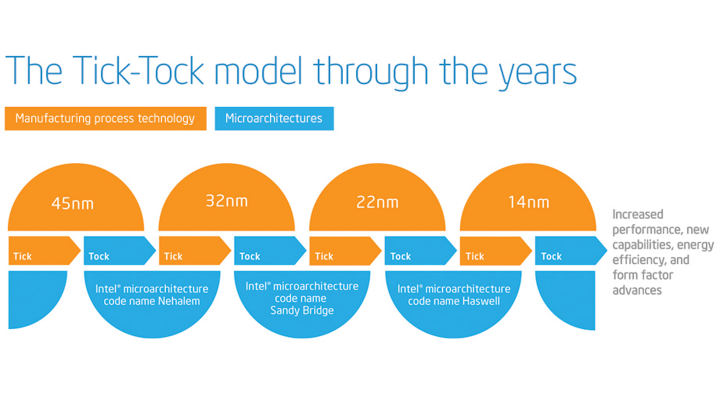
\includegraphics[width=.8\textwidth]{\locpath/figures/chap1/intel_tick_tock.png}
\caption{Intel Tick-Tock model}
\label{fig:1_HPC:intel_tick_tock}
\end{center}
\end{figure}
Since the creation of the Tick-Tock model, it always followed the same fashion: a new manufacturing technology, such as shrinking the chip with better engraving, on a "Tick" followed by a "Tock" which delivers a new micro-architecture.
The Intel processors for HPC are called Xeon and feature ECC memory, higher number of cores, large RAM support, large cache-memory, Hyper-threading, etc. 
Compared to desktop processors, their performances are of a different magnitude.
Intel has given every new processor a code name. 
The last generations are chronologically called Westemere (2011), Sandy Bridge (2012), Ivy Bridge(2013), Haswell (2014), Broadwell (2015), Skylake (2015) and Kaby lake (2016). 

Kaby Lake, the last architecture provided, does not exactly fit the typical "Tick-Tock" process because it is just based on optimizations of the Skylake architecture. 
The Kaby Lake is produced like Skylake with an engraving of 14 nm.
The Tick-Tock model appears to be hard to maintain due to the difficulties to engrave in less than 10 nm with quantum tunneling. 
This leads to using larger many-cores architecture and the bases of the next supercomputer evolutions, the road-map to hybrid models. 

\paragraph{Hyper-threading}
\index{Hyper-threading}
Another specificity of Intel Xeon processors is Hyper-threading (HT). 
This technology makes a single physical processing unit (core) appearing as two logical ones for the user's level.
In fact, a processor embedding 8 cores appears as a 16 cores for user. 
Adding more computation per node can technically allow the cores to switch context when data are fetched from the memory using the processor 100\% during all the computation. 
Multiple studies have been published on HT from Intel itself~\cite{marr2002hyperthreading} to independent researchers~\cite{bononi2006exploring,leng2002empirical}.
This optimization does not fit to all the cases of applications and can be disabled for normal use of the processors in the context of general purpose HPC architectures.

\subsubsection{ARM}
\index{Advanced RISC architecture}
Back in the 1980s, ARM stood for Acorn RISC Machine in reference to the first company to implement this kind of architecture, Acorn Computers. 
This company later changed the name to Advanced RISC Machine (ARM). 
ARM is a specific kind of processors based on RISC architecture as its ISA, despite usual processors using CISC.
The downside of CISC machines are they are difficult to create and they require way more transistor and thus more energy to work. 
The ISA from the RISC is simpler and requires multiple many transistors to operate and thus a smaller silicon area on the die.
Therefore, the energy required and the heat dissipated is less important. 
It becomes easier to create massively parallel processors based on ARM. 
On the other hand, simple ISA imposes more work on the source code compilation to fit the simple architecture. 
This makes the instructions sources longer, and therefore, more single instructions to execute. 

The ARM company provides several versions of ARM processors named Cortex-A7X (2015), Cortex-A5X (2014) and Cortex-A3X (2015) featured for highest-performances, for balancing performances and efficiency or for less power consumption, respectively. 

\index{Mont-Blanc project}
The new ARMv8 architecture starts to provide the tools to target HPC context~\cite{rico2017arm}.
The European approach towards energy efficient HPC, Mont-Blanc project\footnote{http://montblanc-project.eu/}, already constructs ARM based supercomputers. 
The exascale project in Horizon 2020 this project focuses on using ARM-based systems for HPC with many famous contributors, such as Atos/Bull as a project coordinator, ARM, French Alternative Energies and Atomic Energy Commission (CEA), Barcelona Supercomputing Center (BSC), etc.
The project is separated into several steps to finally reach Exascale near 2020. 
The last step, Mont-Blanc 3, is about to work on a pre-Exascale prototype powered by Cavium’s ThunderX2 ARM chip based on 64-bits ARMv8.

\subsection{Intel Xeon Phi}
\index{Xeon Phi}
Another specific HPC product from Intel is the Xeon Phi. 
This device can be considered as a Host or Device/Accelerator machine. 
Intel describes it as "a bootable host processor that delivers massive parallelism and vectorization".
This architecture embed multiple multi-cores processors interconnected and is called Intel's Many Integrated Core (MIC).
We placed this architecture here because it provides hundreds of conventional computation core but the program counter is not shared between them. 
It does not fit in the many-core architecture but is a step in the multi-core one. 
This is the technology on which Intel bases its Exascale machines. 

The architectures names are Knights Ferry, Knights Corner and Knight Landing~\cite{sodani2016knights}. 
The last architecture, Knight Hill, was recently canceled by Intel due to low performances and to focus the Xeon Phi for Exascale.
The main advantage of this architecture compared to GPGPUs is the x86 compatibility of the embedded cores and the fact this device can boot and use to drive other accelerators. 
They also feature more complex operations and handle double precision natively.

\subsection{Many-core architecture, SIMT execution model}
\index{Single Instruction Multiple Threads}
Several architectures can be defined as many-cores and follow the SIMD model from Flynn taxonomy.
These devices integrate thousands of cores that are usually control by fewer control units. 
We can consider these cores as "simpler" since they have to work synchronously and under the coordination of a control unit.
Some devices are specific like the Xeon Phi of Intel, integrating a hundred of regular processor cores which can work independently. 

\subsubsection{GPU}
\index{Graphics Processing Unit}
A CPU can usually have two to 32 computation cores that can operate on different instruction streams, but the SIMT architecture of the GPU is slightly different. 
The cores are grouped and must share the same instruction at the same clock time, but different groups can have their own instructions. 

\begin{figure}
\begin{center}
% classical processor
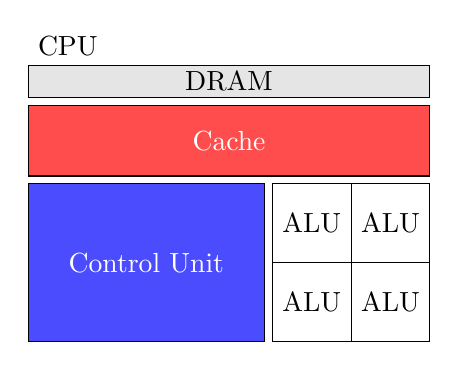
\begin{tikzpicture}
% ALUs
\foreach \x in {3,...,4}
	\foreach \y in {0,...,1}
		\draw[] (\x+.1,\y) rectangle (\x+1.1,\y+1) node[pos=.5] {ALU};
% Control Unit
\draw[fill=blue!70] (0,0) rectangle (3,2) node[pos=.5,text=white] {Control Unit};
%Cache
\draw[fill=red!70] (0,2.1) rectangle (5.1,3) node[pos=.5,text=white] {Cache};
% DRAM
\draw[fill=black!10] (0,3.1) rectangle (5.1,3.5) node[pos=.5] {DRAM};
%Name 
\node[yshift=7pt,anchor=west] at (0,3.5) {CPU};
\end{tikzpicture}
\hspace{1cm}
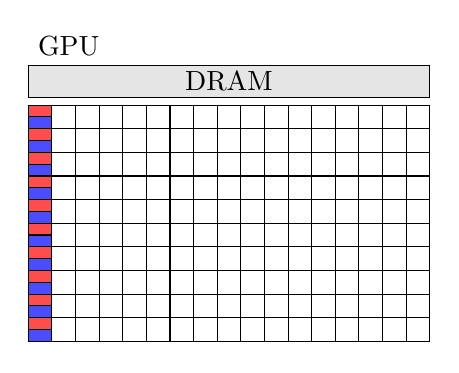
\begin{tikzpicture}
% ALUs
\foreach \y in {0,...,9}
{
	\draw[fill=blue!70] (0,\y * .3) rectangle (.3,\y * .3 + .15) node[pos=.5] {};
	\draw[fill=red!70] (0,\y * .3 + .15) rectangle (.3,\y * .3 + .3) node[pos=.5] {};
	\foreach \x in {1,...,16}
		\draw[] (\x*.3,\y*.3) rectangle (\x *.3+.3,\y*.3+.3) node[pos=.5] {};
}
% DRAM
\draw[fill=black!10] (0,3.1) rectangle (5.1,3.5) node[pos=.5] {DRAM};
% Name 
\node[yshift=7pt,anchor=west] at (0,3.5) {GPU};
\end{tikzpicture}
\end{center}
\caption{Multi-core versus Many-core architecture, case of GPUs}
\label{fig:2_HARD:gpu}
\end{figure}

Figure~\ref{fig:2_HARD:gpu} present the vision between CPU and GPU processors. 
We note in this figure that the usual topology with the ALU lined up in front of their control unit and shared cache memory. 
Every ALU has its own memory and registers to operate local computations. 

These devices are called General Purpose Graphics Processing Units (GPGPUs). 
They are derivative from classical GPUs used for graphical purpose.
Pioneers show that GPGPUs can be use efficiently for classical scientific computations.
The vendor provides then specific GPU for general purpose computing.  
We present here the two main companies providing GPGPUs for HPC world: NVIDIA and AMD.

\paragraph{NVIDIA GPU architecture}
\index{NVIDIA}
The NVIDIA company was founded in April 1993 in Santa Clara, Carolina by three persons, one being the current CEO, Jensen Huang.
The company name originated from \textit{invidia} the Latin word for Envy and vision for graphical rendering. 

NVIDIA is known as the pioneer in graphics, cryptocurrency, portable devices, and now Artificial Intelligence (IA) and appears to be even the creator of the name "GPU".
NVIDIA's GPUs, inspired from visualization and gaming at a first glance, are available as a dedicated device for HPC purpose since the company released the brand named \textit{Tesla}. 
The public GPUs can also be used for dedicated computation, but does not feature ECC memory, double precision or special functions/FFT cores. 
The different versions of the architecture are named following famous physicists, chronologically: Tesla, Fermi, Kepler, Maxwell, Pascal and Volta.

\index{K20Xm}
We describe here the Kepler brand GPU and more specifically the K20Xm GPU on which we based our study. 
\begin{figure}
\centering
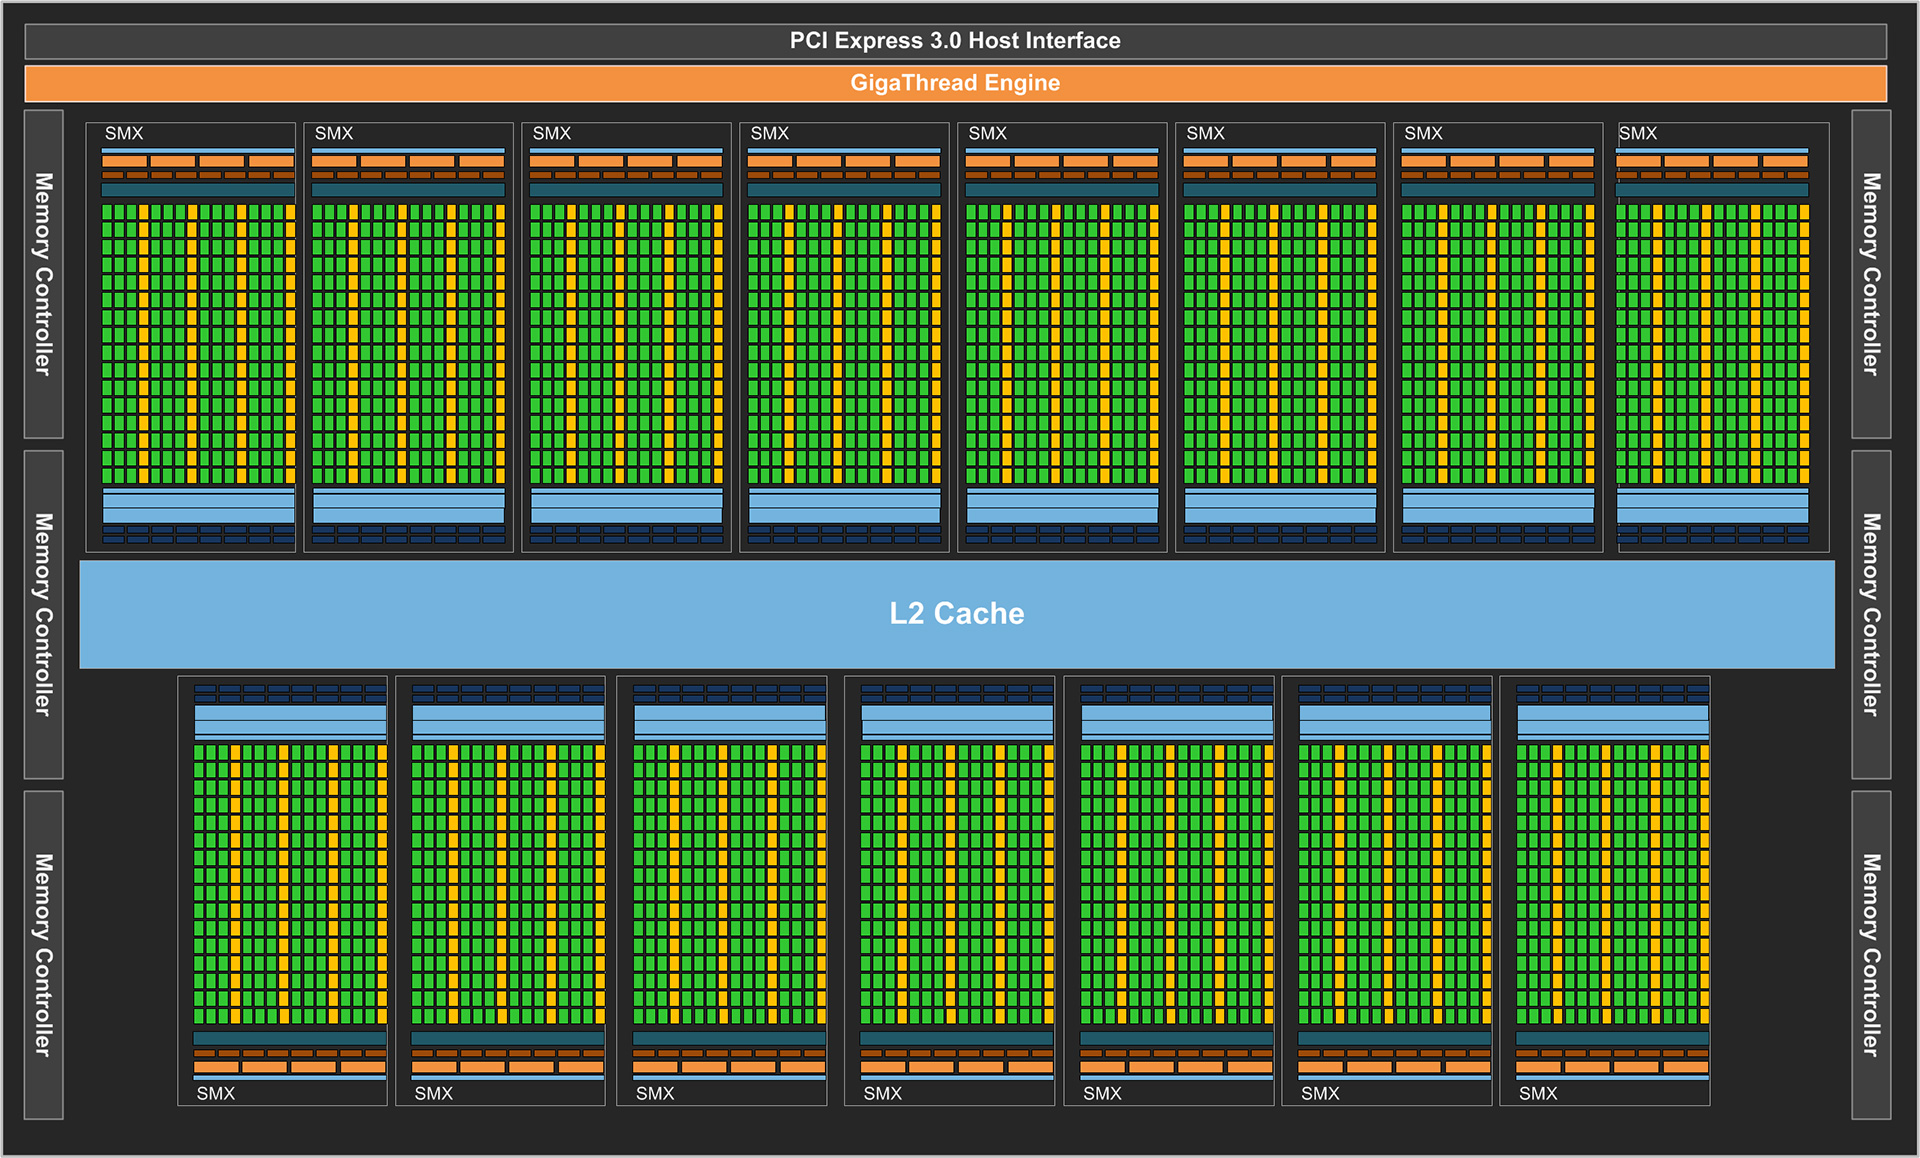
\includegraphics[width=\textwidth]{\locpath/figures/chap1/kepler_architecture.jpeg}
\caption{NVIDIA Tesla Kepler architecture. Single-precision in green and double-precision in yellow}
\label{fig:2_HARD:kepler_arch}
\end{figure}
This NVIDIA Tesla Kepler GPU is based on the GK110 graphics processor describes in the white-paper\cite{nvidia2012nvidias} on 28nm process.
The figure~\ref{fig:2_HARD:kepler_arch} is a representation of the physical elements of this graphics processor. 
The K20X comes in active and passive cooling mode with K20Xc and K20Xm, respectively.
This GPU embeds 2688 CUDA cores distributed in 14 SMX (we note that GK110 normally provides 15 SMX but only 14 are present on the K20X).
In this model each SMX contains 192 single precisions cores, 64 double precision cores, 32 special function units and 32 load/store units.
In a SMX the memory provides 65536 32-bits registers, 64 KB of shared memory L1 cache, 48 KB of read-only cache
The L2 cache is 1546 KB shared by the SMX for a total of 6 GB of memory adding the DRAM.
The whole memory is protected using Single‐Error Correct Double‐Error Detect (SECDED) ECC code.
The power consumption is estimated to 225 W.
This GPGPU is expected to produce 1.31 TFLOPS for double-precision and 3.95 TFLOPS of single-precision.

\paragraph{AMD}
\index{AMD}
Another company is providing GPUs for HPC, Advanced Micro Devices (AMD). 
In front of the huge success of NVIDIA GPU that leads from far the HPC market, it is hard for AMD to find a place for its GPGPUs, the FirePro, in HPC. 
The FirePro is targeted using a language near CUDA, not held by a single company by NVIDIA like CUDA, called OpenCL. 
An interesting creation of AMD is the Accelerated Processing Units (APUs) which embedded the processor and the GPU on the same die since 2011. 
This solution allows them to target the same memory. 

In the race to market and performances, AMD found an accord with Intel to provide dies featuring Intel processor, AMD GPU and common HBM memory. 
The project is call Kaby Lake-G and announced it would be available in the first semester of 2018 for public, not HPC itself. 

\subsubsection{PEZY}
\index{PEZY}
Another many-core architecture only appeared in the last benchmarks. 
The PEZY Super Computer 2, PEZY-SC2, is the third many-core microprocessor developed by the company PEZY. 
The three first machines ranked in the GREEN500 list are accelerator using this many-core die. 
We also note that in the November 2017 list, the fourth supercomputer, Gyoukou, is also powered by PEZY-SC2 cards.

\subsection{Other architectures}
Numerous architectures have not been presented here because they are out of scope of this study. 
We present here two technologies we have encountered in our researches and that may be tomorrow solution for Exascale in HPC. 
\subsubsection{FPGA}
\index{Field Programmable Gates Array}
Field Programmable Gates Array (FPGA) are devices that can be reprogram to fit the needs of the user after their construction.
The leader were historically Altera with the Stratix, Arria and Cyclone FPGAs, which is now part of Intel. 
With the FPGAs, the users have access to the hardware and can design their own circuits. 
Currently, FPGA can be targeted with OpenCL programming language. 
The arrival of Intel in this market assures the best hopes for HPC version of FPGAs. 
The main gap for users is the circuit building that can be designed for specific needs but may be hard to setup. 
\subsubsection{ASIC}
\index{Application Specified Integrated Circuits}
Application Specified Integrated Circuits are dedicated device construct for on purpose. 
An example of ASIC is the Gravity Pipe (GRAPE) which is dedicated to compute gravitation given mass and positions.
Google leads the way for ASIC and recently created its dedicated devices to boost AI bots.
ASIC may be found in some optimized communication devices, such as fast interconnection network in HPC.  

\section{Distributed architectures}

The technologies presented in previous part is the milestone of supercomputers. 
They are used together in a whole system to create machine delivering incredible computational power.

\subsection{Architecture of a supercomputer}
From the hardware described before, we can create the architecture of a cluster from the smallest unit, cores, nodes, to the whole system.

\begin{description}[noitemsep,nolistsep]
\item[Core:] A core is the smallest unit in our devices. 
It refers to the Von Neumann model in case of core with ALU and CU. 
We can separate cores from CPU to GPU, the first one able to be independent whereas the second ones working together and share the same program counter. 
\item[Socket/Host:] A socket is mistakenly called a CPU in current language. 
It is, for multi-cores sockets, composed of several cores. 
The name Host comes from the Host-Device architecture using accelerators. 
\item[Accelerators/Devices:] Accelerators are devices that, when attached to the Host, provide additional computational power. 
We can identify them as GPUs, FPGAs, ASICs, etc. 
A socket can have access to one or more accelerators and can also share the accelerator usage. 
\item[Computation node: ] The next layer of our HPC system is the computation node, which is a group of several sockets and accelerators sharing memory;
\item[Rack: ] A rack is a set of computation nodes, generally in vertical stack. 
It may also include specific nodes dedicated to the network or the Input/Output.
\item[Interconnection: ] The nodes are grouped together with hard wire connection following a specific interconnection topology with very high bandwidth.
\item[System/Cluster/Supercomputer] The cluster group several racks though an interconnection network.
\end{description}

An interconnect technology is required in order to connect nodes together and allow distributed programming. 
Interconnection networks are the way the nodes of a cluster are connected together. 

\subsection{Interconnection topologies}
\index{Interconnect}
Several topologies exist from point to point to multi-dimensional torus.
%
\begin{figure}[t!]
\centering
\resizebox {.14\columnwidth} {!} {
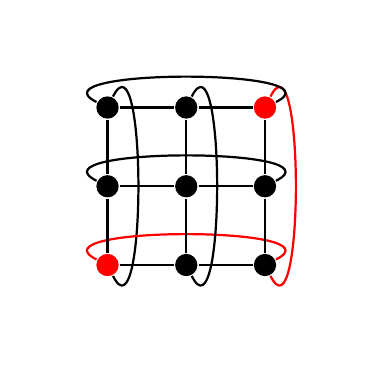
\begin{tikzpicture}[thick,inner sep=0.1cm]
	\node [fill,circle,red] (node 1000) at (0,0) {};
	\node [fill,circle] (node 1001) at (1,0) {};
	\node [fill,circle] (node 1002) at (2,0) {};
	\node [fill,circle] (node 1003) at (0,1) {};
	\node [fill,circle] (node 1004) at (1,1) {};
	\node [fill,circle] (node 1005) at (2,1) {};
	\node [fill,circle] (node 1006) at (0,2) {};
	\node [fill,circle] (node 1007) at (1,2) {};
	\node [fill,circle,red] (node 1008) at (2,2) {};
	
	\draw (node 1000)
							         .. controls +(0.500000,-1.000000)
							                 and +(0.500000,1.000000)
							         .. (node 1006);
	\draw[red] (node 1000)
							         .. controls +(-1.000000,0.500000)
							                 and +(1.000000,0.500000)
							         .. (node 1002);
	\draw (node 1000) -- (node 1001);
	\draw (node 1000) -- (node 1003);
	\draw (node 1001) -- (node 1004);
	\draw (node 1001)
							         .. controls +(0.500000,-1.000000)
							                 and +(0.500000,1.000000)
							         .. (node 1007);
	\draw (node 1002) -- (node 1005);
	\draw (node 1002) -- (node 1001);
	\draw[red] (node 1002)
							         .. controls +(0.500000,-1.000000)
							                 and +(0.500000,1.000000)
							         .. (node 1008);
	
	\draw (node 1003)
							         .. controls +(-1.000000,0.500000)
							                 and +(1.000000,0.500000)
							         .. (node 1005);
	\draw (node 1003) -- (node 1006);
	\draw (node 1003) -- (node 1004);
	\draw (node 1004) -- (node 1005);
	\draw (node 1004) -- (node 1007);
	\draw (node 1005) -- (node 1008);
	\draw (node 1006)
							         .. controls +(-1.000000,0.500000)
							                 and +(1.000000,0.500000)
							         .. (node 1008);
	\draw (node 1006) -- (node 1007);
	\draw (node 1007) -- (node 1008);
\end{tikzpicture}
}
%\vspace{1cm}
\resizebox {.34\columnwidth} {!} {
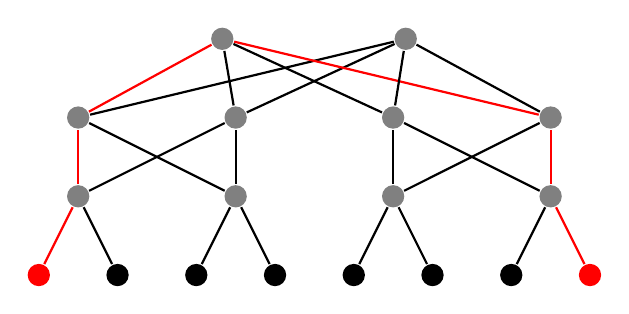
\begin{tikzpicture}[thick,inner sep=0.1cm]
	
	\node [fill,circle,red] (node a) at (0,0) {};
	\node [fill,circle] (node b) at (1,0) {};
	\node [fill,circle] (node c) at (2,0) {};
	\node [fill,circle] (node d) at (3,0) {};
	\node [fill,circle] (node e) at (4,0) {};
	\node [fill,circle] (node f) at (5,0) {};
	\node [fill,circle] (node g) at (6,0) {};
	\node [fill,circle,red] (node h) at (7,0) {};

	\node [fill,circle,black!50] (node a0) at (0.5,1) {};
	\node [fill,circle,black!50] (node a1) at (2.5,1) {};
	\node [fill,circle,black!50] (node a2) at (4.5,1) {};
	\node [fill,circle,black!50] (node a3) at (6.5,1) {};
	\node [fill,circle,black!50] (node a4) at (0.5,2) {};
	\node [fill,circle,black!50] (node a5) at (2.5,2) {};
	\node [fill,circle,black!50] (node a6) at (4.5,2) {};
	\node [fill,circle,black!50] (node a7) at (6.5,2) {};

	\node [fill,circle,black!50] (node n0) at (2.33,3) {};
	\node [fill,circle,black!50] (node n1) at (4.66,3) {};

	\draw[red] (node a) -- (node a0);
	\draw (node b) -- (node a0);
	\draw (node c) -- (node a1);
	\draw (node d) -- (node a1);
	\draw (node e) -- (node a2);
	\draw (node f) -- (node a2);
	\draw (node g) -- (node a3);
	\draw[red] (node h) -- (node a3);

	\draw[red] (node a0) -- (node a4);
	\draw (node a0) -- (node a5);
	\draw (node a1) -- (node a4);
	\draw (node a1) -- (node a5);
	\draw (node a2) -- (node a6);
	\draw (node a2) -- (node a7);
	\draw (node a3) -- (node a6);
	\draw[red] (node a3) -- (node a7);

	\draw[red] (node n0) -- (node a4);
	\draw (node n1) -- (node a5);
	\draw (node n0) -- (node a5);
	\draw (node n1) -- (node a4);
	\draw (node n0) -- (node a6);
	\draw (node n1) -- (node a7);
	\draw[red] (node n0) -- (node a7);
	\draw (node n1) -- (node a6);
\end{tikzpicture}
}
%\caption{Torus and 4-ary tree}
%\end{figure}
%\begin{figure}
\resizebox {.24\columnwidth} {!} {
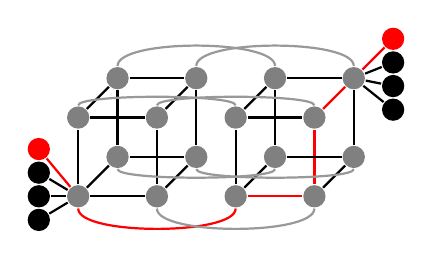
\begin{tikzpicture}[thick,inner sep=0.1cm]
	
	\node [fill,circle,black!50] (node a0) at (0,0) {};
	\node [fill,circle,black!50] (node b0) at (1,0) {};
	\node [fill,circle,black!50] (node c0) at (0,1) {};
	\node [fill,circle,black!50] (node d0) at (1,1) {};
	\node [fill,circle,black!50] (node e0) at (0.5,0.5) {};
	\node [fill,circle,black!50] (node f0) at (1.5,0.5) {};
	\node [fill,circle,black!50] (node g0) at (0.5,1.5) {};
	\node [fill,circle,black!50] (node h0) at (1.5,1.5) {};

	\node [fill,circle,black!50] (node a1) at (2,0) {};
	\node [fill,circle,black!50] (node b1) at (3,0) {};
	\node [fill,circle,black!50] (node c1) at (2,1) {};
	\node [fill,circle,black!50] (node d1) at (3,1) {};
	\node [fill,circle,black!50] (node e1) at (2.5,0.5) {};
	\node [fill,circle,black!50] (node f1) at (3.5,0.5) {};
	\node [fill,circle,black!50] (node g1) at (2.5,1.5) {};
	\node [fill,circle,black!50] (node h1) at (3.5,1.5) {};

	\node [fill,circle,red] (node cn0) at (4,2.) {};
	\node [fill,circle] (node cn1) at (4,1.7) {};
	\node [fill,circle] (node cn2) at (4,1.4) {};
	\node [fill,circle] (node cn3) at (4,1.1) {};

	\node [fill,circle] (node cn4) at (-0.5,-0.3) {};
	\node [fill,circle] (node cn5) at (-0.5,0.0) {};
	\node [fill,circle] (node cn6) at (-0.5,0.3) {};
	\node [fill,circle,red] (node cn7) at (-0.5,0.6) {};


	\draw (node a0) -- (node b0);
	\draw (node b0) -- (node d0);
	\draw (node c0) -- (node d0);
	\draw (node a0) -- (node c0);
	\draw (node e0) -- (node f0);
	\draw (node f0) -- (node h0);
	\draw (node g0) -- (node h0);
	\draw (node e0) -- (node g0);

	\draw (node a0) -- (node e0);
	\draw (node b0) -- (node f0);
	\draw (node c0) -- (node g0);
	\draw (node d0) -- (node h0);

	\draw[red] (node a1) -- (node b1);
	\draw[red] (node b1) -- (node d1);
	\draw (node c1) -- (node d1);
	\draw (node a1) -- (node c1);
	\draw (node e1) -- (node f1);
	\draw (node f1) -- (node h1);
	\draw (node g1) -- (node h1);
	\draw (node e1) -- (node g1);

	\draw (node a1) -- (node e1);
	\draw (node b1) -- (node f1);
	\draw (node c1) -- (node g1);
	\draw[red] (node d1) -- (node h1);

	\draw[red] (node cn0) -- (node h1);
	\draw (node cn1) -- (node h1);
	\draw (node cn2) -- (node h1);
	\draw (node cn3) -- (node h1);
	\draw (node cn4) -- (node a0);
	\draw (node cn5) -- (node a0);
	\draw (node cn6) -- (node a0);
	\draw[red] (node cn7) -- (node a0);

	%\draw (node a0) -- (node a1);
	\draw[red] (node a0)
		        .. controls +(0.,-0.500000)
		                 and +(0.,-0.500000)
		        .. (node a1);
	\draw[black!40] (node b0) 
				.. controls +(0.,-0.500000)
		                 and +(0.,-0.500000)
		        .. (node b1);
	\draw[black!40] (node c0) 
				.. controls +(0.,0.300000)
		                 and +(0.,0.300000)
		        ..  (node c1);
	\draw[black!40] (node d0) 
				.. controls +(0.,0.300000)
		                 and +(0.,0.300000)
		        ..  (node d1);
	\draw[black!40] (node e0) 
				.. controls +(0.,-0.300000)
		                 and +(0.,-0.300000)
		        ..  (node e1);
	\draw[black!40] (node f0) 
				.. controls +(0.,-0.300000)
		                 and +(0.,-0.300000)
		        ..  (node f1);
	\draw[black!40] (node g0) 
				.. controls +(0.,0.500000)
		                 and +(0.,0.500000)
		        ..  (node g1);
	\draw[black!40] (node h0) 
				.. controls +(0.,0.500000)
		                 and +(0.,0.500000)
		        ..  (node h1);
\end{tikzpicture}
}
%\hspace{1cm}
\resizebox {.24\columnwidth} {!} {
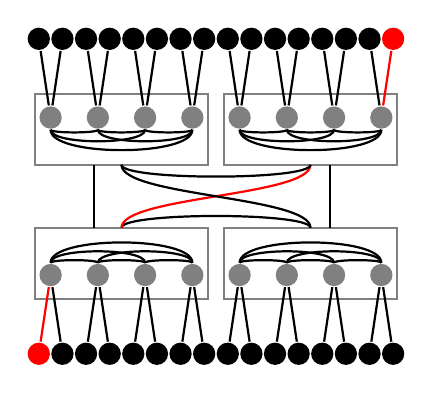
\begin{tikzpicture}[thick,inner sep=0.1cm]
	\node [fill,circle,black!50] (node a00) at (0.45,1) {};
	\node [fill,circle,black!50] (node a01) at (1.05,1) {};
	\node [fill,circle,black!50] (node a02) at (1.65,1) {};
	\node [fill,circle,black!50] (node a03) at (2.25,1) {};
	\node [fill,circle,red] (node n01) at (0.3,0) {};
	\node [fill,circle] (node n02) at (0.6,0) {};
	\node [fill,circle] (node n03) at (0.9,0) {};
	\node [fill,circle] (node n04) at (1.2,0) {};
	\node [fill,circle] (node n05) at (1.5,0) {};
	\node [fill,circle] (node n06) at (1.8,0) {};
	\node [fill,circle] (node n07) at (2.1,0) {};
	\node [fill,circle] (node n08) at (2.4,0) {};

	\node [fill,circle,black!50] (node a10) at (2.85,1) {};
	\node [fill,circle,black!50] (node a11) at (3.45,1) {};
	\node [fill,circle,black!50] (node a12) at (4.05,1) {};
	\node [fill,circle,black!50] (node a13) at (4.65,1) {};
	\node [fill,circle] (node n11) at (2.7,0) {};
	\node [fill,circle] (node n12) at (3,0) {};
	\node [fill,circle] (node n13) at (3.3,0) {};
	\node [fill,circle] (node n14) at (3.6,0) {};
	\node [fill,circle] (node n15) at (3.9,0) {};
	\node [fill,circle] (node n16) at (4.2,0) {};
	\node [fill,circle] (node n17) at (4.5,0) {};
	\node [fill,circle] (node n18) at (4.8,0) {};

	\node [fill,circle,black!50] (node a20) at (0.45,3) {};
	\node [fill,circle,black!50] (node a21) at (1.05,3) {};
	\node [fill,circle,black!50] (node a22) at (1.65,3) {};
	\node [fill,circle,black!50] (node a23) at (2.25,3) {};
	\node [fill,circle] (node n21) at (0.3,4) {};
	\node [fill,circle] (node n22) at (0.6,4) {};
	\node [fill,circle] (node n23) at (0.9,4) {};
	\node [fill,circle] (node n24) at (1.2,4) {};
	\node [fill,circle] (node n25) at (1.5,4) {};
	\node [fill,circle] (node n26) at (1.8,4) {};
	\node [fill,circle] (node n27) at (2.1,4) {};
	\node [fill,circle] (node n28) at (2.4,4) {};

	\node [fill,circle,black!50] (node a30) at (2.85,3) {};
	\node [fill,circle,black!50] (node a31) at (3.45,3) {};
	\node [fill,circle,black!50] (node a32) at (4.05,3) {};
	\node [fill,circle,black!50] (node a33) at (4.65,3) {};
	\node [fill,circle] (node n31) at (2.7,4) {};
	\node [fill,circle] (node n32) at (3,4) {};
	\node [fill,circle] (node n33) at (3.3,4) {};
	\node [fill,circle] (node n34) at (3.6,4) {};
	\node [fill,circle] (node n35) at (3.9,4) {};
	\node [fill,circle] (node n36) at (4.2,4) {};
	\node [fill,circle] (node n37) at (4.5,4) {};
	\node [fill,circle,red] (node n38) at (4.8,4) {};

	\draw[black!50] (2.65,2.4) rectangle (4.85,3.3);
	\draw[black!50] (0.25,2.4) rectangle (2.45,3.3);

	\draw[black!50] (2.65,0.7) rectangle (4.85,1.6);
	\draw[black!50] (0.25,0.7) rectangle (2.45,1.6);

	\draw (1.35,1.6)
	.. controls +(0.,0.2)
	    and +(0.,0.2)
	..  (3.75,1.6); 

	\draw[red] (1.35,1.6)
	.. controls +(0.,0.4)
	    and +(0.,-0.4)
	..  (3.75,2.4); 
	%\draw (1.35,1.6) -- (3.75,2.4);
	\draw (3.75,1.6)
	.. controls +(0.,0.4)
	    and +(0.,-0.4)
	..  (1.35,2.4); 
	%\draw (3.75,1.6) -- (1.35,2.4);

	\draw (1.,1.6) -- (1.,2.4);
	\draw (4.,1.6) -- (4.,2.4);

	\draw (1.35,2.4)
	.. controls +(0.,-0.2)
	    and +(0.,-0.2)
	..  (3.75,2.4); 


	\draw[red] (node n01) -- (node a00);
	\draw (node n02) -- (node a00);
	\draw (node n03) -- (node a01);
	\draw (node n04) -- (node a01);
	\draw (node n05) -- (node a02);
	\draw (node n06) -- (node a02);
	\draw (node n07) -- (node a03);
	\draw (node n08) -- (node a03);

	\draw (node n11) -- (node a10);
	\draw (node n12) -- (node a10);
	\draw (node n13) -- (node a11);
	\draw (node n14) -- (node a11);
	\draw (node n15) -- (node a12);
	\draw (node n16) -- (node a12);
	\draw (node n17) -- (node a13);
	\draw (node n18) -- (node a13);

	\draw (node n21) -- (node a20);
	\draw (node n22) -- (node a20);
	\draw (node n23) -- (node a21);
	\draw (node n24) -- (node a21);
	\draw (node n25) -- (node a22);
	\draw (node n26) -- (node a22);
	\draw (node n27) -- (node a23);
	\draw (node n28) -- (node a23);

	\draw (node n31) -- (node a30);
	\draw (node n32) -- (node a30);
	\draw (node n33) -- (node a31);
	\draw (node n34) -- (node a31);
	\draw (node n35) -- (node a32);
	\draw (node n36) -- (node a32);
	\draw (node n37) -- (node a33);
	\draw[red] (node n38) -- (node a33);

	\draw (node a00) 
	.. controls +(0.,0.2)
	    and +(0.,0.2)
	..  (node a01);
	\draw (node a00) 
	.. controls +(0.,0.35)
	    and +(0.,0.35)
	..  (node a02);
	\draw (node a00) 
	.. controls +(0.,0.5)
	    and +(0.,0.5)
	..  (node a03);
	\draw (node a01) 
	.. controls +(0.,0.2)
	    and +(0.,0.2)
	..  (node a02);
	\draw (node a01) 
	.. controls +(0.,0.35)
	    and +(0.,0.35)
	..  (node a03);
	\draw (node a02) 
	.. controls +(0.,0.2)
	    and +(0.,0.2)
	..  (node a03);

	\draw (node a10) 
	.. controls +(0.,0.2)
	    and +(0.,0.2)
	..  (node a11);
	\draw (node a10) 
	.. controls +(0.,0.35)
	    and +(0.,0.35)
	..  (node a12);
	\draw (node a10) 
	.. controls +(0.,0.5)
	    and +(0.,0.5)
	..  (node a13);
	\draw (node a11) 
	.. controls +(0.,0.2)
	    and +(0.,0.2)
	..  (node a12);
	\draw (node a11) 
	.. controls +(0.,0.35)
	    and +(0.,0.35)
	..  (node a13);
	\draw (node a12) 
	.. controls +(0.,0.2)
	    and +(0.,0.2)
	..  (node a13);

	\draw (node a20) 
	.. controls +(0.,-0.2)
	    and +(0.,-0.2)
	..  (node a21);
	\draw (node a20) 
	.. controls +(0.,-0.35)
	    and +(0.,-0.35)
	..  (node a22);
	\draw (node a20) 
	.. controls +(0.,-0.5)
	    and +(0.,-0.5)
	..  (node a23);
	\draw (node a21) 
	.. controls +(0.,-0.2)
	    and +(0.,-0.2)
	..  (node a22);
	\draw (node a21) 
	.. controls +(0.,-0.35)
	    and +(0.,-0.35)
	..  (node a23);
	\draw (node a22) 
	.. controls +(0.,-0.2)
	    and +(0.,-0.2)
	..  (node a23);

	\draw (node a30) 
	.. controls +(0.,-0.2)
	    and +(0.,-0.2)
	..  (node a31);
	\draw (node a30) 
	.. controls +(0.,-0.35)
	    and +(0.,-0.35)
	..  (node a32);
	\draw (node a30) 
	.. controls +(0.,-0.5)
	    and +(0.,-0.5)
	..  (node a33);
	\draw (node a31) 
	.. controls +(0.,-0.2)
	    and +(0.,-0.2)
	..  (node a32);
	\draw (node a31) 
	.. controls +(0.,-0.35)
	    and +(0.,-0.35)
	..  (node a33);
	\draw (node a32) 
	.. controls +(0.,-0.2)
	    and +(0.,-0.2)
	..  (node a33);
\end{tikzpicture}
}
\caption{Torus, Fat-Tree, HyperX, DragonFly}
\label{fig:1_HPC:topology}
\end{figure}
%
The figure~\ref{fig:1_HPC:topology} is a representation of famous topologies. 
Each interconnect technology has its own specificity. 
These networks take in account the number of nodes to interconnect and the targeted bandwidth/budget.
Several declination of each network are not detailed here. 
The Mesh and the Torus are used as a basis in lower layers of others more complex interconnection networks. 
A perfect example is the supercomputer called K-Computer describe in the next section.
The Fat Tree presented here is a k-ary Fat Tree, the higher the position in the tree, the more connections are found and with a bandwidth being important. 
The nodes are available as the leaves, on the middle level we find the switches and on top the routers. 
This is the topology of the ROMEO supercomputer we used for our tests. 
Another topology, HyperX\cite{ahn2009hyperx}, is based on Hyper-Cube.
The DragonFly\cite{kim2008technology} interconnect is recent, 2008, and is used in modern day supercomputers.

InfiniBand (IB)\index{Infiniband} is the most widespread technology used for interconnection with different kind of bandwidth presented in figure~\ref{fig:1_HPC:infiniband}.
It provides high bandwidth and small latency and companies such as Intel, Mellanox, etc. provide directly adapters and switches specifically for IB. 

\begin{table}[t!]
\begin{center}
\[\arraycolsep=0.pt\def\arraystretch{1.2}
\begin{tabular}{| l | l | l || l | l | l | }
\hline
\textbf{Name} & \textbf{Gbs} & \textbf{Year} & \textbf{Name} & \textbf{Gbs} & \textbf{Year} \\
\hline
\hline
Single DR & 2.5 & 2003 & Enhanced DR & 25 & 2014 \\
\hline
Double DR & 5 & 2005 & Highg DR & 50 & 2017 \\
\hline
Quad DR & 10 & 2007 & Next DR & 100 & 2020 \\
\hline
Fourth DR & 14 & 2011 & & &  \\
\hline
\end{tabular}
\]
\caption{InfiniBand technologies name, year and bandwidth}
\label{fig:1_HPC:infiniband}
\end{center}
\end{table}

Unfortunately, this augmentation of clock rate is not sustainable due to the energy required and the heat generated by the running component. 
Another idea originated in the 19th century with the first multi-core processors. 


\subsection{Remarkable supercomputers}
The TOP500\footnote{\url{https://www.top500.org}} is the reference benchmarks for the world rank supercomputers. 
This benchmark is based on the LINPACK and aim to solve a dense system of linear equations.
Most of the TOP10 machines have specific architectures and, of course, the most efficient ones. 
In this section, we describe several supercomputers about their interconnect, processors and specific accelerators. 

\subsubsection{Sunway Taihulight}
\index{Sunway Taihulight}
Sunway Taihulight is the third Chinese supercomputer to be ranked in the first position of the TOP500 list, in November 2017. 
A recent report from Jack J. Dongarra, a figure in HPC, decrypted the architecture of this supercomputer\cite{dongarra2016report}. 
The most interesting point is the conception of this machine, completely done in China. 
The Sunway CPUs were designed and built in China by the Shanghai High Performance IC Design Center. 

\begin{figure}[t!]
\centering
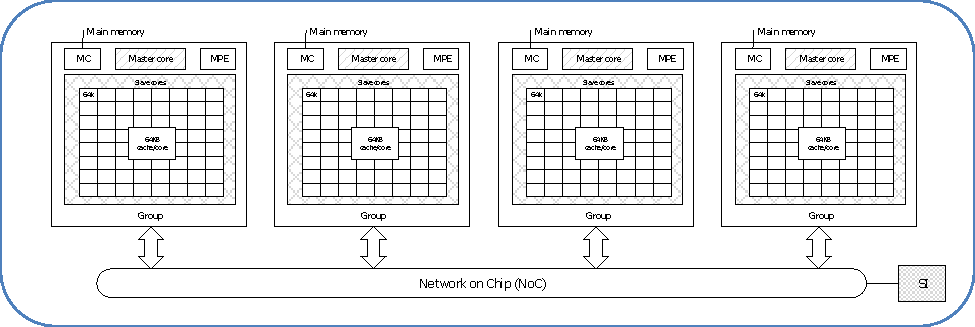
\includegraphics[scale=1]{\locpath/figures/Chap1/report_sunway_CPE}
\caption{Sunway Taihulight node architecture from \textit{Report on the Sunway TaihuLight System}, Jack Dongarra, June 24, 2016.}
\label{fig:chap1_report_sunway_CPE}
\end{figure}

The SW26010, a many core architecture processor, features 260 cores based on RISC architecture and a specific conception, depicted on figure~\ref{fig:chap1_report_sunway_CPE}. 
The processor is composed of the master core, a Memory Controller (MC) and a Management Processing Element (MPE) that manages the Computing Processing Elements (CPE), which are the slaves’ cores. 

The interconnect network is called Sunway Network and is connected using Mellanox Host Channel Adapter (HCA) and switches. 
This is a five-level interconnect going through computing nodes, computing board, super-nodes and cabinets to the complete system.
For the latest TOP500 list, from November 2017, the total memory is 1.31 PB and the number of cores available is 10,649,600.
The peak performance is 125.4 PFLOPS but the Linpack is only 93 PFLOPS which is 74.16\% of theoretic efficiency. 

\subsubsection{Piz Daint}
\index{Piz Daint}
The supercomputer of the CSCS, Swiss National Supercomputing Center, is currently ranked second on the November 2017 TOP500 list. 
This GPUs accelerated supercomputer is a most powerful representative of GPU hybrid acceleration and is the most powerful European supercomputer. 
This supercomputer is composed of 4761 hybrids and 1210 multi-core nodes. 
\index{NVIDIA}
There are hybrids nodes embedding an Intel Xeon E5-2690v3 and an NVIDIA Tesla Pascal P100 GPGPU. 
The interconnect is based on a Dragonfly network topology and Cray Aries routing and communications ASICs. 
The peak performance is 25.326 TFLOPS using only the hybrid nodes with Linpack generating 19.590 TFLOPS.
The low power consumption ranks Piz Daint as tenth in the November 2017 GREEN500.

\subsubsection{K-Computer}
\index{K-Computer}
The K-Computer was the top 1 supercomputer of the 2011 TOP500. 
The TOFU interconnect network makes the K-Computer unique~\cite{ajima2009tofu} and stands for TOrus FUsion.
\begin{figure}[t!]
\begin{center}
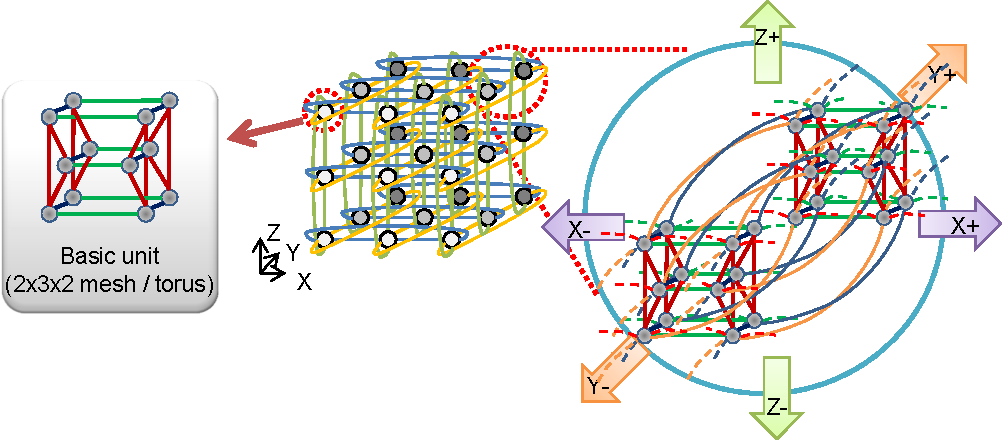
\includegraphics[width=\textwidth]{\locpath/figures/chap1/6d_torus}
\end{center}
\caption{TOFU Interconnect schematic from \textit{The K-Computer: System Overview}, Atsuya Uno, SC11}
\label{fig:1_HPC:tofu}
\end{figure}
\index{Interconnection}
This interconnect presented in figure~\ref{fig:1_HPC:tofu} mixes a 6D Mesh/Torus interconnect.
The basic units are based on a mesh and are interconnected together in a three-dimensional torus. 
In this configuration, each node can access to its 12 neighbors directly. 
It also provide a fault tolerant network with many routes to reach distant node. 

%\todo{AJouter MIRA/SEQUOIA pour paler de IBM, pour le Graph500 = meilleurs supercomputers}
%\todo{Parler de CRAY ?}
\subsubsection{Sequoia/Mira}
\index{IBM BlueGene}
The Sequoia supercomputer was ranked first on the 2012 TOP500 list. 
It is based on BlueGene from IBM.
The BlueGene project made up to three main architectures with BlueGene/L, BlueGene/P and BlueGene/Q.
It is very interesting to note the BlueGene architecture because 15 machine utilizing this architecture were in the top 200 in the last GRAPH500 list in November 2017.
The algorithm used on these supercomputers will be our basis in the Part II regarding our implementation of the GRAPH500 benchmark.

\section{ROMEO Supercomputer}
\index{ROMEO Supercomputer}
The ROMEO supercomputer center is the computation center of the Champagne-Ardenne region in France. 
Hosted since 2002 by the University of Reims Champagne-Ardenne, this so called meso-center (Medium size HPC center) is used for HPC in theoretic research and domain science like applied mathematics, physics, biophysics and chemistry. 

This project is supported by Europe, National Fundings, Grand-Est region and Reims Metropole. 
It aims to host research and production codes of the region for industrial, research and academics purposes. 

We are currently working on the fourth version of ROMEO, last updated in 2013. 
As many of our tests in this study have been done on this machine, we will carefully describe its architecture. 

This supercomputer was ranked 151st in the TOP500 and fifth in the GREEN500 list. 

\subsection{ROMEO hardware architecture}
\label{sec:part1_ROMEO}
ROMEO is a Bull/Atos supercomputer composed of 130 BullX R421 computing nodes. 

\index{K20Xm}
Each node is composed of two processors Intel Ivy Bridge 8 cores @ 2,6 GHz. 
Each processor has access to 16 GB of memory for a total of 32 GB per node, the total memory of 4.160 TB. 
Each processor is linked, using PCIe-v3, to an NVIDIA Tesla K20Xm GPGPU. 
This cluster provides then 260 processors for a total of 2080 CPU cores and 260 GPGPU providing 698880 GPU cores. 
The computation nodes are interconnected with an Infiniband QDR non-blocking network structured as a FatTree. 
The Infiniband is a QDR providing 10 GB/s. 

The storage for users is 57 TB and the cluster also provide 195 GB of Lustre and 88TB of parallel scratch file-system. 

In addition to the 130 computations nodes, the cluster provides a visualization node NVIDIA GRID with two K2 cards and 250GB of DDR3 RAM. 
The old machine, renamed Clovis, is also available but does not features GPUs. 

The supercomputer supports MPI with GPU Aware and GPUDirect. 

ROMEO is based on the Slurm\footnote{\url{https://slurm.schedmd.com/}} workload manager for node distribution among the users. 
This manager allows different usage of the cluster with classical reservation-submission or more asynchronous computation with best-effort. 
We developed advantages of both submissions systems in Part II. 

\subsection{New ROMEO supercomputer, June 2018}

In June 2018 a new version of the supercomputer ROMEO will be installed at the University of Reims Champagne Ardenne. 
This project intents to feature a supercomputer ranked around 250th in TOP500. 
It is a renewed partnership between ATOS/BULL and NVIDIA. 

The new ROMEO will feature 115 computation nodes with a total of 3220 CPU cores. 
The technology selected is the BULL \textit{Sequana} with its high energy saving, BXI network technology, NVLink support for GPUs and the density of the cluster. 
Each node will provide a Skylake 6132 CPU with 14 cores with a maximum frequency of 2.6GHz.

Two different types of node are present: 
\begin{itemize}[noitemsep,nolistsep]
\item[-] 70 of the with 4 GPUs and 96GB of RAM featuring a total of 280 Pascal P100 SMX2 GPUs.
\item[-] 45 last generation Intel CPUs with 192GB of memory per CPU. 
\end{itemize}

The machine will feature up to 15.3TB of global memory. 

The aim is to provide a performance of 964.6 TFLOPS in LINPACK and to be present in several TOP500 lists with a starting position around 232th or 297th. 

\section{Conclusion}

In this chapter, we reviewed the most important modern day hardware architectures and technologies. 
In order to use the driver or API in the most efficient way, we need to keep in mind the way the data and instructions are proceed by the machine. 

Efficiency is based on computation power, but also communications, we showed different interconnection topologies and their specificities. 
We present perfect use cases of the technologies in the current top ranked systems.
We show that every architecture is unique in its construction and justify the optimization work dedicated to reach performance. 

We determine from the new technologies presented here that supercomputers are moving toward hybrids architectures featuring multi-core processors accelerated by one or more devices such as many-core architectures. 
The Exascale supercomputer of 2020 will be shaped using hybrid architectures and they represent the best of nowadays technology for purpose of HPC this day and age. 
Combining CPU and GPUs or FPGA on the same die and sharing the same memory space may also be another solution.



\chapter*{Conclusion}
In this part we presented the 
% Conclusion
\addcontentsline{toc}{chapter}{Conclusion and future works}
\markboth{CONCLUSION AND FUTURE WORKS}{}
\chapter*{Conclusion}

% Annexes
%\addcontentsline{toc}{chapter}{Annexes}
%\chapter*{Annexes}

% Bibliography,
\addcontentsline{toc}{chapter}{Bibliography}
\bibliographystyle{alpha}
%\nocite{*}
\bibliography{biblio/my_papers.bib,biblio/biblio_langford,biblio/biblio_graph,biblio/biblio_sph,biblio/biblio_hpc,biblio/biblio_part2_chap1}

\pagenumbering{gobble}
% index just in case it is useful 
%\addcontentsline{toc}{chapter}{Index}
%\printindex
\newgeometry{left=1cm,right=1cm,top=1cm,bottom=1.5cm}

\markboth{}{}
\cleartoleftpage
\addcontentsline{toc}{chapter}{Abstract}
\hrule
\vspace{.2cm}
Titre français: \textbf{\phdTitleFR}
\vspace{.2cm}
\hrule
\vspace{.3cm}

La course à l'Exascale est entamée et tous les pays du monde rivalisent pour présenter un supercalculateur exaflopique à l'horizon 2020-2021. 
Ces superordinateurs vont servir à des fins militaires, pour montrer la puissance d'une nation, mais aussi pour des recherches sur le climat, la santé, l'automobile, physique, astrophysique et bien d'autres domaines d'application. 
Ces supercalculateurs de demain doivent respecter une enveloppe énergétique de 1 MW pour des raisons à la fois économiques et environnementales. 
Pour arriver à produire une telle machine, les architectures classiques doivent évoluer vers des machines hybrides équipées d'accélérateurs tels que les GPU, Xeon Phi, FPGA, etc. 

Nous montrons que les benchmarks actuels ne nous semblent pas suffisants pour cibler ces applications qui ont un comportement irrégulier. 
Cette étude met en place une métrique ciblant les aspects limitants des architectures de calcul: le calcul et les communications avec un comportement irrégulier. 

Le problème mettant en avant la complexité de calcul est le problème académique de Langford. 
Pour la communication nous proposons notre implémentation du benchmark du Graph500.
Ces deux métriques mettent clairement en avant l'avantage de l'utilisation d'accélérateurs, comme des GPUs, dans ces circonstances spécifiques et limitantes pour le HPC. 
Pour valider notre thèse nous proposons l'étude d'un problème réel mettant en jeu à la fois le calcul, les communications et une irrégularité extrême. 
En réalisant des simulations de physique et d'astrophysique nous montrons une nouvelle fois l'avantage de l'architecture hybride et sa scalabilité. 

\vspace{.3cm}
\hrule
\vspace{.1cm}

{
\small
Mots clés: Calcul Haute Performance, Architecture Hybrides, Simulation
}

\vspace{.1cm}
\hrule

\vspace{.4cm}
\hrule
\vspace{.2cm}
English title: \textbf{\phdTitleEN}
\vspace{.2cm}
\hrule
\vspace{.3cm}

The countries of the world are already competing for Exascale and the first exaflopics supercomputer should be release by 2020-2021.
These supercomputers will be used for military purposes, to show the power of a nation, but also for research on climate, health, physics, astrophysics and many other areas of application.
These supercomputers of tomorrow must respect an energy envelope of 1 MW for reasons both economic and environmental.
In order to create such a machine, conventional architectures must evolve to hybrid machines equipped with accelerators such as GPU, Xeon Phi, FPGA, etc.

We show that the current benchmarks do not seem sufficient to target these applications which have an irregular behavior.
This study sets up a metrics targeting the walls of computational architectures: computation and communication walls with irregular behavior.
The problem for the computational wall is the Langford's academic combinatorial problem.
We propose our implementation of the Graph500 benchmark in order to target the communication wall.

These two metrics clearly highlight the advantage of using accelerators, such as GPUs, in these specific and representative problems of HPC.
In order to validate our thesis we propose the study of a real problem bringing into play at the same time the computation, the communications and an extreme irregularity.
By performing simulations of physics and astrophysics we show once again the advantage of the hybrid architecture and its scalability.

\vspace{.3cm}
\hrule
\vspace{.1cm}

{
\small
Key works: High Performance Computing, Hybrid Architectures, Simulation
}

\vspace{.1cm}
\hrule

\vspace{.3cm}
\textbf{Discipline: \phdDiscipline}

\textbf{Spécialité: \phdSpeciality}
\vspace{.2cm}

\hspace{8cm}Université de Reims Champagne Ardenne

\hspace{8cm}Laboratoire du CReSTIC EA 3804

\hspace{8cm}UFR Sciences Exactes et Naturelles, 

\hspace{8cm}Moulin de la Housse, 51867 Reims




\end{document}
